% Options for packages loaded elsewhere
\PassOptionsToPackage{unicode}{hyperref}
\PassOptionsToPackage{hyphens}{url}
%
\documentclass[
]{book}
\usepackage{lmodern}
\usepackage{amssymb,amsmath}
\usepackage{ifxetex,ifluatex}
\ifnum 0\ifxetex 1\fi\ifluatex 1\fi=0 % if pdftex
  \usepackage[T1]{fontenc}
  \usepackage[utf8]{inputenc}
  \usepackage{textcomp} % provide euro and other symbols
\else % if luatex or xetex
  \usepackage{unicode-math}
  \defaultfontfeatures{Scale=MatchLowercase}
  \defaultfontfeatures[\rmfamily]{Ligatures=TeX,Scale=1}
\fi
% Use upquote if available, for straight quotes in verbatim environments
\IfFileExists{upquote.sty}{\usepackage{upquote}}{}
\IfFileExists{microtype.sty}{% use microtype if available
  \usepackage[]{microtype}
  \UseMicrotypeSet[protrusion]{basicmath} % disable protrusion for tt fonts
}{}
\makeatletter
\@ifundefined{KOMAClassName}{% if non-KOMA class
  \IfFileExists{parskip.sty}{%
    \usepackage{parskip}
  }{% else
    \setlength{\parindent}{0pt}
    \setlength{\parskip}{6pt plus 2pt minus 1pt}}
}{% if KOMA class
  \KOMAoptions{parskip=half}}
\makeatother
\usepackage{xcolor}
\IfFileExists{xurl.sty}{\usepackage{xurl}}{} % add URL line breaks if available
\IfFileExists{bookmark.sty}{\usepackage{bookmark}}{\usepackage{hyperref}}
\hypersetup{
  pdftitle={STICS intercrop: a work in progress for the ReMIX H2020 project},
  pdfauthor={R. Vezy},
  hidelinks,
  pdfcreator={LaTeX via pandoc}}
\urlstyle{same} % disable monospaced font for URLs
\usepackage{color}
\usepackage{fancyvrb}
\newcommand{\VerbBar}{|}
\newcommand{\VERB}{\Verb[commandchars=\\\{\}]}
\DefineVerbatimEnvironment{Highlighting}{Verbatim}{commandchars=\\\{\}}
% Add ',fontsize=\small' for more characters per line
\usepackage{framed}
\definecolor{shadecolor}{RGB}{248,248,248}
\newenvironment{Shaded}{\begin{snugshade}}{\end{snugshade}}
\newcommand{\AlertTok}[1]{\textcolor[rgb]{0.94,0.16,0.16}{#1}}
\newcommand{\AnnotationTok}[1]{\textcolor[rgb]{0.56,0.35,0.01}{\textbf{\textit{#1}}}}
\newcommand{\AttributeTok}[1]{\textcolor[rgb]{0.77,0.63,0.00}{#1}}
\newcommand{\BaseNTok}[1]{\textcolor[rgb]{0.00,0.00,0.81}{#1}}
\newcommand{\BuiltInTok}[1]{#1}
\newcommand{\CharTok}[1]{\textcolor[rgb]{0.31,0.60,0.02}{#1}}
\newcommand{\CommentTok}[1]{\textcolor[rgb]{0.56,0.35,0.01}{\textit{#1}}}
\newcommand{\CommentVarTok}[1]{\textcolor[rgb]{0.56,0.35,0.01}{\textbf{\textit{#1}}}}
\newcommand{\ConstantTok}[1]{\textcolor[rgb]{0.00,0.00,0.00}{#1}}
\newcommand{\ControlFlowTok}[1]{\textcolor[rgb]{0.13,0.29,0.53}{\textbf{#1}}}
\newcommand{\DataTypeTok}[1]{\textcolor[rgb]{0.13,0.29,0.53}{#1}}
\newcommand{\DecValTok}[1]{\textcolor[rgb]{0.00,0.00,0.81}{#1}}
\newcommand{\DocumentationTok}[1]{\textcolor[rgb]{0.56,0.35,0.01}{\textbf{\textit{#1}}}}
\newcommand{\ErrorTok}[1]{\textcolor[rgb]{0.64,0.00,0.00}{\textbf{#1}}}
\newcommand{\ExtensionTok}[1]{#1}
\newcommand{\FloatTok}[1]{\textcolor[rgb]{0.00,0.00,0.81}{#1}}
\newcommand{\FunctionTok}[1]{\textcolor[rgb]{0.00,0.00,0.00}{#1}}
\newcommand{\ImportTok}[1]{#1}
\newcommand{\InformationTok}[1]{\textcolor[rgb]{0.56,0.35,0.01}{\textbf{\textit{#1}}}}
\newcommand{\KeywordTok}[1]{\textcolor[rgb]{0.13,0.29,0.53}{\textbf{#1}}}
\newcommand{\NormalTok}[1]{#1}
\newcommand{\OperatorTok}[1]{\textcolor[rgb]{0.81,0.36,0.00}{\textbf{#1}}}
\newcommand{\OtherTok}[1]{\textcolor[rgb]{0.56,0.35,0.01}{#1}}
\newcommand{\PreprocessorTok}[1]{\textcolor[rgb]{0.56,0.35,0.01}{\textit{#1}}}
\newcommand{\RegionMarkerTok}[1]{#1}
\newcommand{\SpecialCharTok}[1]{\textcolor[rgb]{0.00,0.00,0.00}{#1}}
\newcommand{\SpecialStringTok}[1]{\textcolor[rgb]{0.31,0.60,0.02}{#1}}
\newcommand{\StringTok}[1]{\textcolor[rgb]{0.31,0.60,0.02}{#1}}
\newcommand{\VariableTok}[1]{\textcolor[rgb]{0.00,0.00,0.00}{#1}}
\newcommand{\VerbatimStringTok}[1]{\textcolor[rgb]{0.31,0.60,0.02}{#1}}
\newcommand{\WarningTok}[1]{\textcolor[rgb]{0.56,0.35,0.01}{\textbf{\textit{#1}}}}
\usepackage{longtable,booktabs}
% Correct order of tables after \paragraph or \subparagraph
\usepackage{etoolbox}
\makeatletter
\patchcmd\longtable{\par}{\if@noskipsec\mbox{}\fi\par}{}{}
\makeatother
% Allow footnotes in longtable head/foot
\IfFileExists{footnotehyper.sty}{\usepackage{footnotehyper}}{\usepackage{footnote}}
\makesavenoteenv{longtable}
\usepackage{graphicx,grffile}
\makeatletter
\def\maxwidth{\ifdim\Gin@nat@width>\linewidth\linewidth\else\Gin@nat@width\fi}
\def\maxheight{\ifdim\Gin@nat@height>\textheight\textheight\else\Gin@nat@height\fi}
\makeatother
% Scale images if necessary, so that they will not overflow the page
% margins by default, and it is still possible to overwrite the defaults
% using explicit options in \includegraphics[width, height, ...]{}
\setkeys{Gin}{width=\maxwidth,height=\maxheight,keepaspectratio}
% Set default figure placement to htbp
\makeatletter
\def\fps@figure{htbp}
\makeatother
\setlength{\emergencystretch}{3em} % prevent overfull lines
\providecommand{\tightlist}{%
  \setlength{\itemsep}{0pt}\setlength{\parskip}{0pt}}
\setcounter{secnumdepth}{5}
\usepackage{booktabs}
\usepackage[]{natbib}
\bibliographystyle{apalike}

\title{STICS intercrop: a work in progress for the ReMIX H2020 project}
\author{R. Vezy}
\date{2020-03-31}

\begin{document}
\maketitle

{
\setcounter{tocdepth}{1}
\tableofcontents
}
\hypertarget{prerequisites}{%
\chapter{Prerequisites}\label{prerequisites}}

Each chapter of the book match a specific objective. I first introduce the subject with a brief description, try to find some solutions for the specific issues and show the results.

The code is only visible on the \texttt{html} version of the book, so please refer to this format if you need any further information (open the \texttt{index.html} file).

This book is written using the R \textbf{bookdown} package, which can be installed from CRAN or Github:

To compile this example to PDF, you need XeLaTeX. You are recommended to install TinyTeX (which includes XeLaTeX): \url{https://yihui.name/tinytex/}.

\hypertarget{Light}{%
\chapter{Light Interception}\label{Light}}

\hypertarget{introduction}{%
\section{Introduction}\label{introduction}}

In STICS, the light interception is either computed using a simple Beer law assuming a homogeneous, turbid canopy, or a radiation transfer model that consider the plants leaf area index, canopy shape, height and density. The Beer law option is very simple but generally fairly accurate for high density homogeneous crops, but may rapidly yield unsatisfying predictions for stands with higher structural complexity (e.g.~perennial plantations or mixed crops). For mixed crops, the model uses the radiation transfer model in a particular manner that is described in further details below.

For the case of intercrops, the model first set the taller crop as ``dominant'', and the shorter crop as ``dominated''. The model then compute the radiation interception of each one according to the dominancy, the structure (height, width, light extinction coefficient\ldots) and position (interrow distance, row orientation) of the species. Of course, the dominancy of each plant species can be inverted if the dominated plant become taller than the dominant plant, and the model checks every day for such a case.

\begin{Shaded}
\begin{Highlighting}[]
\NormalTok{j=}\DecValTok{1}              \CommentTok{# julian day (DOY= Day Of Year)}
\NormalTok{ir=}\StringTok{ }\DecValTok{1}            \CommentTok{# Interrow distance}
\NormalTok{l=}\StringTok{ }\FloatTok{0.2}           \CommentTok{# Width of the plant crown}
\NormalTok{rap=}\StringTok{ }\FloatTok{0.5}         \CommentTok{# Thickness to width ratio}
\NormalTok{haut=}\StringTok{ }\FloatTok{1.}         \CommentTok{# Height of the part of the dominant plant above the dominated plant}
                 \CommentTok{# = hauteurzero = P_hautbase-originehaut}
                 \CommentTok{# with originehaut= dominated plant height}
\NormalTok{P_forme=}\StringTok{ }\DecValTok{1}       \CommentTok{# Plant shape code (1= rectangle, 2= upside triangle, 3= downside tr.)}
\NormalTok{alpha=}\StringTok{ }\DecValTok{0}         \CommentTok{# Row orientation}
\NormalTok{lat=}\StringTok{ }\FloatTok{43.61}       \CommentTok{# Latitude in degrees}
\NormalTok{trg=}\StringTok{ }\DecValTok{25}          \CommentTok{# Global radiation}
\NormalTok{rdif=}\StringTok{ }\FloatTok{0.4}        \CommentTok{# Diffuse fraction of the atmospheric radiation}
\NormalTok{P_ktrou=}\StringTok{ }\FloatTok{0.8}     \CommentTok{# Light extinction coefficient of the dominant plant}
\NormalTok{lai=}\StringTok{ }\DecValTok{4}           \CommentTok{# Leaf area index of the dominant plant}
\NormalTok{eai=}\StringTok{ }\DecValTok{0}           \CommentTok{# Equivalent leaf area index, = photosynthetic surface that is not from}
\CommentTok{# leaves (e.g. wheat ears, rapeseed siliquae, pea pods or grapes during their green stage)}
\end{Highlighting}
\end{Shaded}

To facilitate understanding, we will use a common intercrop example throughout the whole document. We take a mixed crop simulated for the day of the year 1 with a global radiation of 25 MJ m-2 day-1 (= 12 MJ m-2 day-1 of PAR), and a diffuse fraction of light of 0.4, an interrow spacing of 1 meter, a shape of 1 (1= rectangle, 2= upside triangle and 3= downside rectangle), a canopy width of 0.2 meter, a canopy thickness of 0.1 meter, a row orientation of 0 relative to the North-South axis at latitude 43.61 degrees north, an LAI of 4, a light extinction coefficient of 0.8. The canopy of the dominant plant is 1 meter above the dominated plant.
All code used in this document can be viewed in each section by clicking on the \texttt{Code} button on the right.

\hypertarget{plant-shape}{%
\section{Plant shape}\label{plant-shape}}

Each plant radiation interception is computed using an approximation of its shape (\texttt{P\_forme}= 1, rectangle, = 2 upside triangle, = 3 downside triangle), leaf area index (\texttt{lai} or \texttt{p(i)\%lai(ens,n)}), height, width, density at emergence and leaf area density (\texttt{dfol}).

\hypertarget{plant-width-computation}{%
\subsection{Plant width computation}\label{plant-width-computation}}

First, the plant width is computed using the \texttt{formplante} function. This computation is possible thanks to the relationship between two ways for computing the plant leaf area, where one of them uses the plant width:

\begin{itemize}
\item
  First, assuming the plant has a square footprint (i.e.~plant projection is square), we can find the plant leaf area using the leaf area index (\texttt{lai}) and the plant density:\\
  \(LA=\frac{\left(lai+laisen+eai\right)}{densite}\) which is the equivalent to: \(LA=\left(lai+laisen+eai\right)\cdot interrang\cdot distrang\)\\
  where \texttt{lai} is the leaf area index, \texttt{laisen} is the senescent leaf area index, \texttt{eai} is the equivalent leaf area of the photosynthetic organs that are not leaves (e.g.~flower buds), \texttt{interrang} is the inter-row spacing and \texttt{distrang} the intra-row distance.
\item
  Second, using the leaf area density and the plant volume such as:\\
  \(LA=dfol\cdot largeur\cdot epaisseur\cdot profondeur\) for a cuboid and \(LA=dfol\cdot\frac{1}{2}\cdot\left(largeur\cdot epaisseur\cdot profondeur\right)\) for a triangular prism, where \texttt{dfol} is the leaf area density, \texttt{largeur} is the \textbf{plant width} (also called \texttt{largtrans}), \texttt{epaisseur} is the plant thickness and \texttt{profondeur} is the plant depth.
\end{itemize}

Knowing both equations, and assuming the two following hypothesis:

\begin{enumerate}
\def\labelenumi{\arabic{enumi}.}
\tightlist
\item
  The plant depth is equal to the plant width
\item
  The intra-row distance between two plants is equal to the plant width
\end{enumerate}

We can now compute the plant width as:\\
\(largeur=\sqrt{\frac{(lai+laisen+eai)\cdot interrang}{dfol\cdot varrapforme}}\)

where \texttt{varrapforme} (or \texttt{raptrans} further) is the ratio between the plant thickness and width and is computed as \(varrapforme=\frac{(hauteur-P_{hautbase})}{largeur}\) where \texttt{hauteur} is the total plant height, \texttt{P\_hautbase} is the plant (i.e.~crown) base height and \texttt{largeur} is the plant width (see fig \ref{fig:Width} for more details)

\begin{figure}
\centering
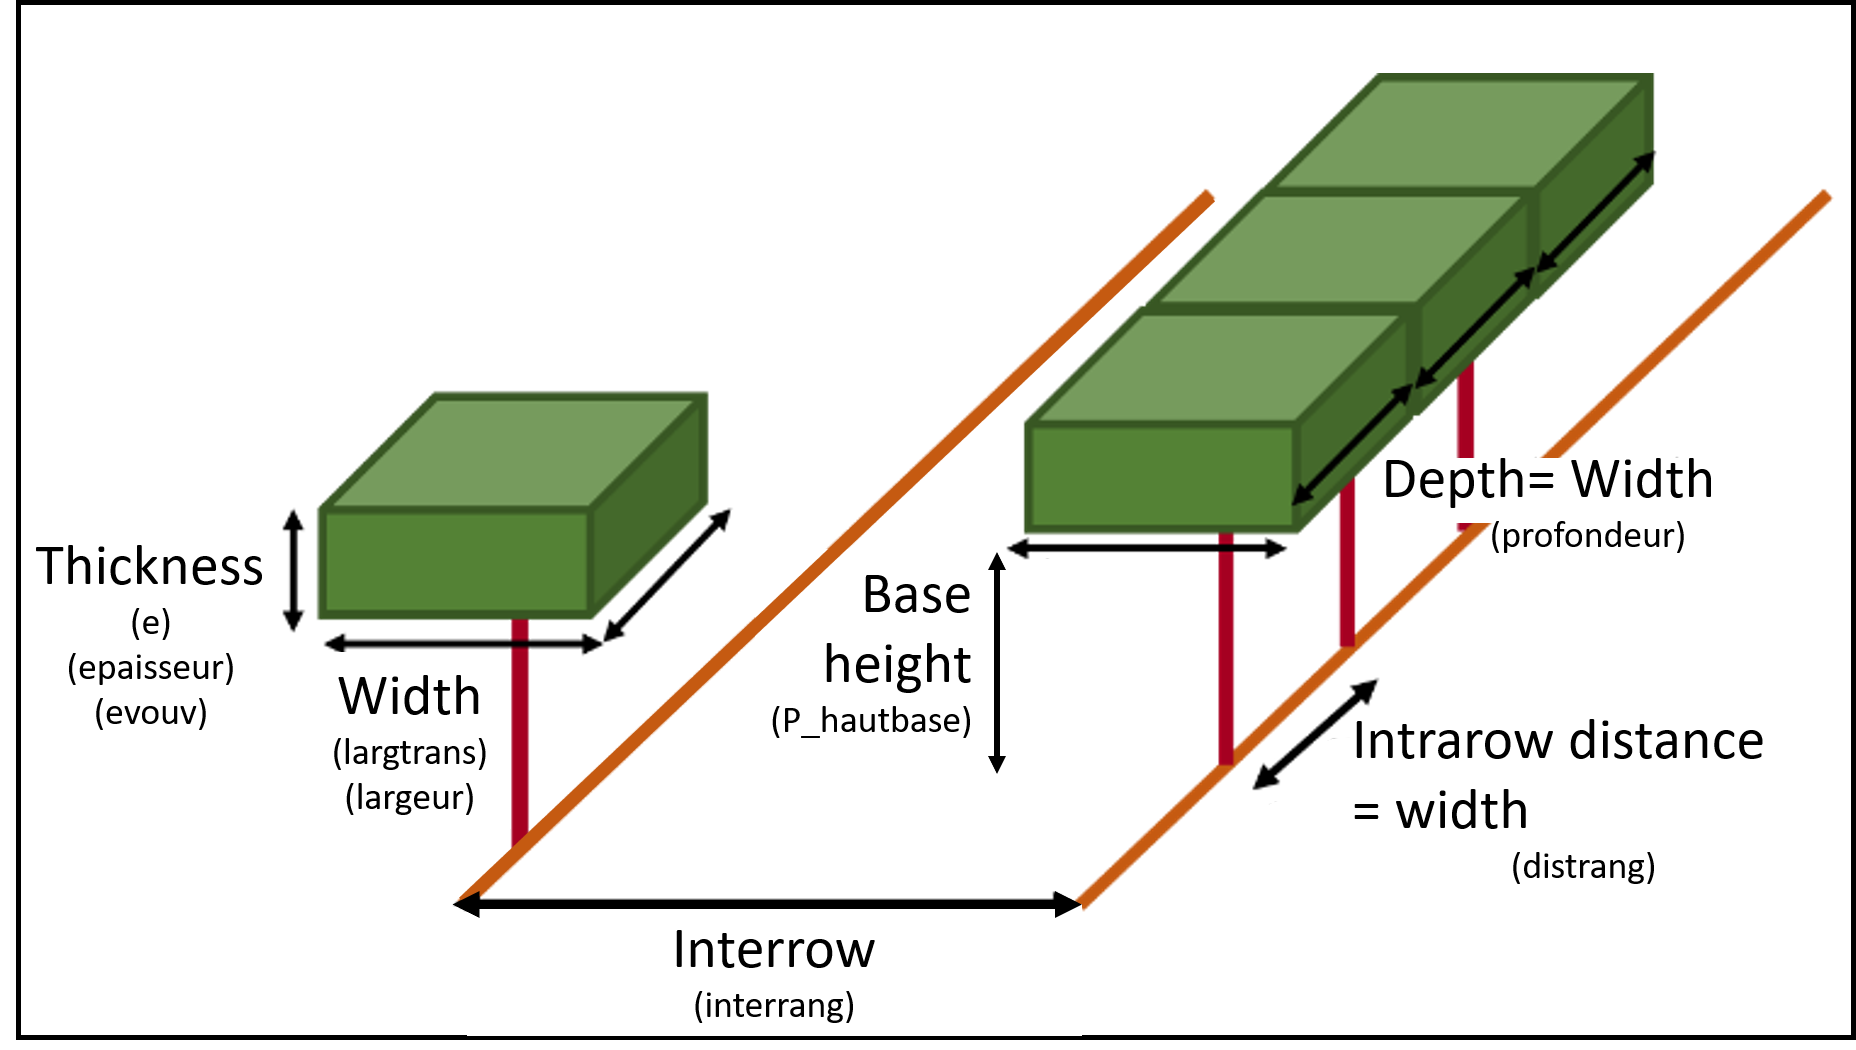
\includegraphics{img/Light-interception-dominant-1.png}
\caption{\label{fig:Width}\textbf{Diagram representing the different parameters used to compute plant width. The different names used in the model are shown between parenthesis}}
\end{figure}

\hypertarget{plant-width-correction}{%
\subsection{Plant width correction}\label{plant-width-correction}}

If the dominated plant is higher than the base height of the dominant plant, the radiation interception of the dominant plant is partially reduced, by reducing the volume that can intercept light to the canopy volume above the dominated plant only. This correction is made to consider the competition for light between the two species, and is computed according to the shape of the plant.

Consequently, the model first compute the height of the dominated plant (\texttt{sc\%originehaut}) by looking for the maximum height between the sunlit and shaded part of the dominated plant:\\
\texttt{sc\%originehaut\ =\ max(p(i+1)\%hauteur(sc\%AO),p(i+1)\%hauteur(sc\%AS))}

\begin{quote}
\texttt{sc\%originehaut} is fixed to \texttt{0} (= soil) while computing the dominated plant.
\end{quote}

Hence, the new thickness (\texttt{enouv}) is computed as: \(enouv=largeur\cdot\left|varrapforme\right|+hauteurzero\), and is used to re-compute the shape of the plant:

\begin{itemize}
\tightlist
\item
  The new thickness to width ratio (\texttt{raptrans}, formerly \texttt{varrapforme}): \(raptrans=\frac{enouv}{largeur}\) for rectangle shaped plants,
\item
  The new width (\texttt{largtrans}, formerly \texttt{largeur}): \(largtrans=\frac{enouv}{varrapforme}\) for upsided triangle shaped plants,
\item
  The new width (\texttt{largtrans}, formerly \texttt{largeur}): \(raptrans=\frac{enouv}{largtrans}\) for downsided triangle shaped plants,
\end{itemize}

All variable names are changed, whether there is a correction or not. Here is a summary table:

\begin{table}

\caption{\label{tab:varmatch}Variable name modification in the formplante function}
\centering
\begin{tabular}[t]{l|l|l}
\hline
Original & Modified & Definition\\
\hline
hauteur & hauteur & Height\\
\hline
largeur & largtrans & Width\\
\hline
varrapforme & raptrans & Thickness/Width Ratio\\
\hline
enouv & enouv & Thickness\\
\hline
\end{tabular}
\end{table}

\begin{quote}
Upside triangle is a triangle with its base at the bottom, while downside triangle is a triangle with the base at the top.
\end{quote}

The correction of the shape of the plant can be summarised in the diagram Presented in Figure \ref{fig:Comprad}.

\begin{figure}
\centering
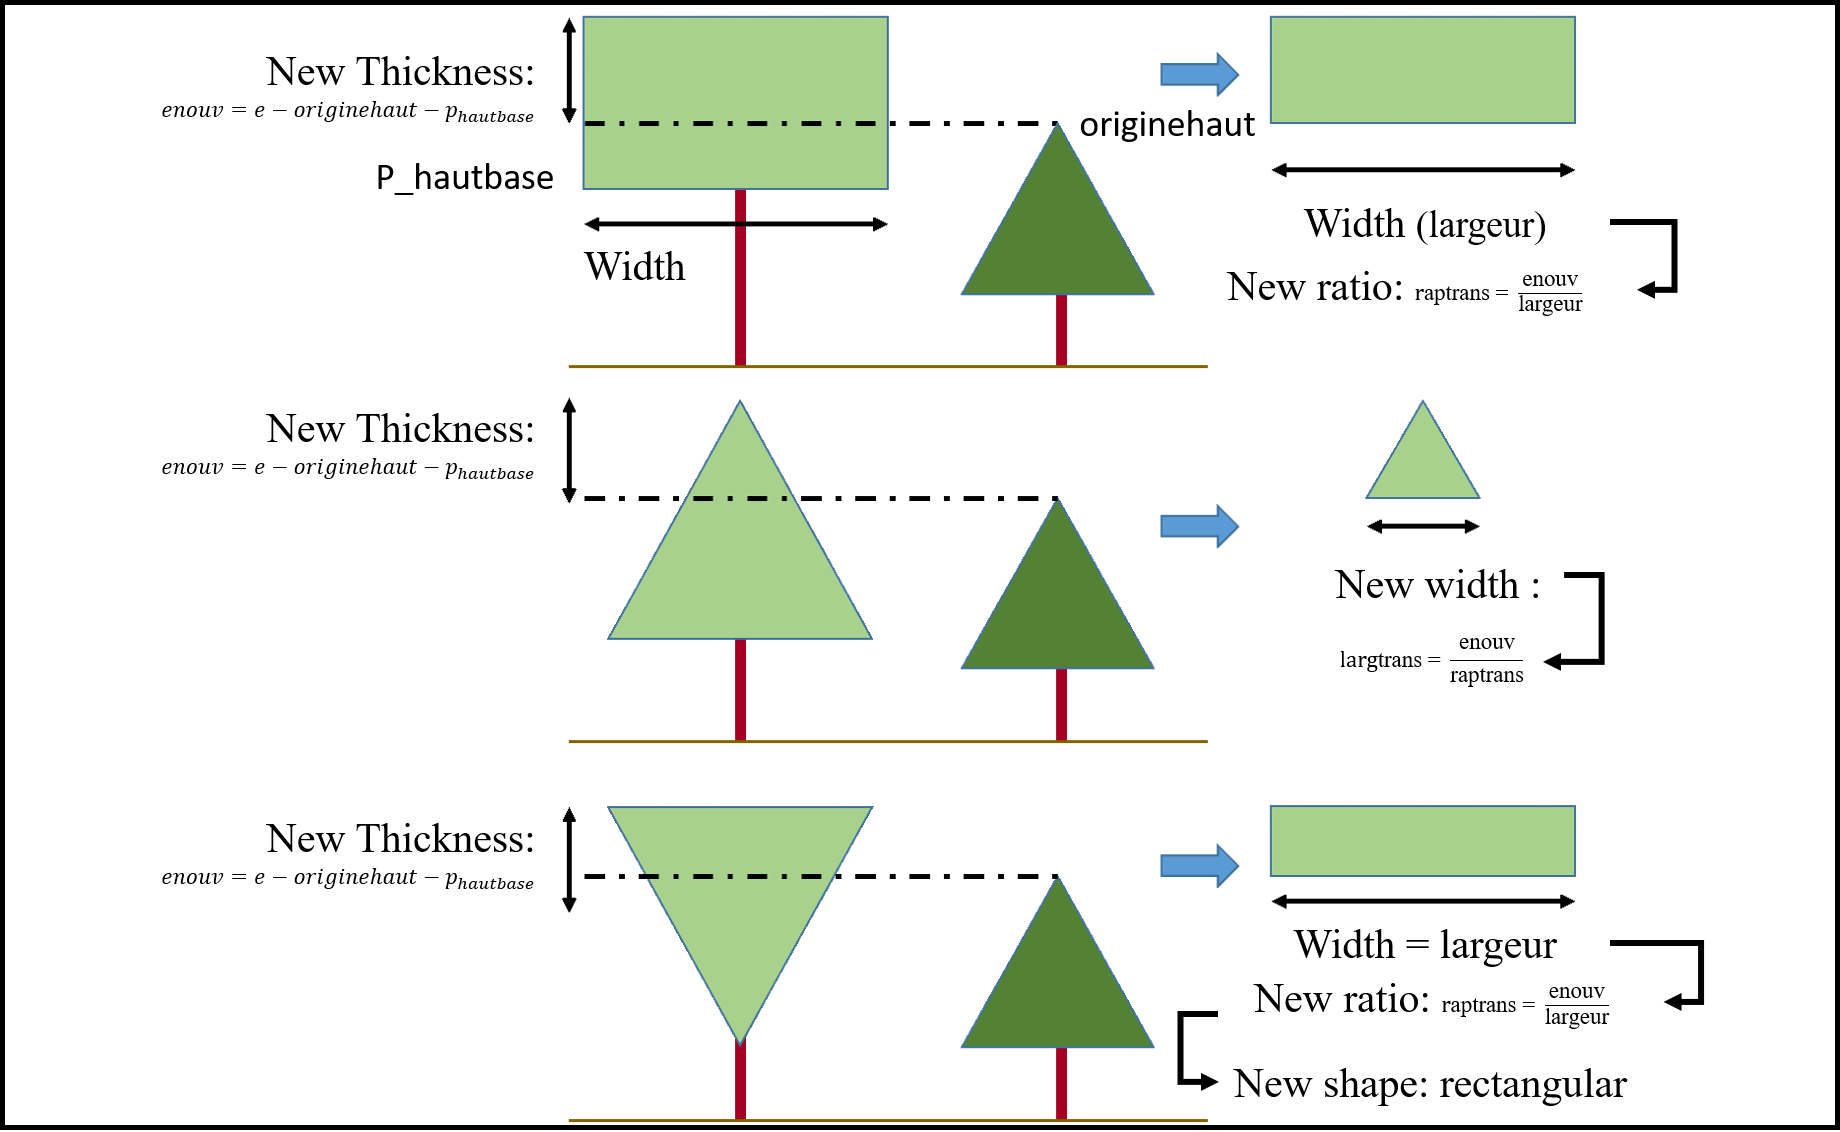
\includegraphics{img/Light-interception-dominant-2.png}
\caption{\label{fig:Comprad}\textbf{Competition for radiation interception of the dominant plant induced by a high dominated plant}}
\end{figure}

The correction of the shape of the plant is only used to compute the light transmitted to a plane at the dominated plant or soil height. The targeted plant interception is computed using its whole leaf area index and a light extinction coefficient.

\hypertarget{plant-height}{%
\subsection{Plant height}\label{plant-height}}

The plant height is simply computed using the plant base height, its width, and the thickness to width ratio:

\(hauteur=P_{hautbase}+largeur\cdot\left|varrapforme\right|\)

So indirectly, the plant height depends on its \texttt{LAI}, because the plant width is computed using it in the first place.
This formalism maybe not optimal, because the plant \texttt{height} and \texttt{LAI} are not well related during advanced plant physiological stages.

\hypertarget{light-interception}{%
\section{Light interception}\label{light-interception}}

The light intercepted by a plant species is obtained by computing the light reaching a horizontal plane below its canopy, either at the height of the dominated plant (for the dominant plant) of the soil (for the dominated plant). Therefore, the light incident on this plane is either coming from:

\begin{itemize}
\tightlist
\item
  The incident light coming from the atmosphere, divided into two components, namely the diffuse and direct light. This light is called \texttt{rdroit} in the model,
\item
  The light transmitted by the dominant crop, which is called \texttt{rtrans}, and that is generally of lower quality for photosynthesis. The effect of light quality is wrapped in the equivalent density formalism, see Chapter \ref{plantdensity} for more details.
\end{itemize}

Consequently, numerous points (20, or 200 if the inter-row is lower than 1 m) are equally distributed every meter along the inter-row (\emph{i.e.} one point every 5 cm, or every 0.5 cm with 200 points), at the height of the plane. These points are used to discretize the computation of the incident light at the surface of the plane.\\
Hence, the total number of points to simulate is computed using the \texttt{interval} parameter, which is equal to 200 if the inter-row is lower than 1 meter or 20 if more. It is then used to compute the total number of points to simulate as: \(N_{points}=\frac{ir}{2}\cdot interval\)

\begin{quote}
In practice, the model really simulates only half of the inter-row, because it is considered that the other half have the same light conditions at daily time-scale. For example, if we take an interrow of 10 meters, the model simulates 100 points equally distributed from 0 to 5 meters.
\end{quote}

Here is an example of the X position on the plane, starting from the left-hand side of the row, using an inter-row spacing of 1 meter and a plant width of 0.2 meter:

\begin{Shaded}
\begin{Highlighting}[]
\ControlFlowTok{if}\NormalTok{(ir}\OperatorTok{<}\FloatTok{1.0}\NormalTok{)\{}
\NormalTok{  interval =}\StringTok{ }\DecValTok{200}
\NormalTok{\}}\ControlFlowTok{else}\NormalTok{\{}
\NormalTok{  interval =}\StringTok{ }\FloatTok{20.}
\NormalTok{\}}
\NormalTok{i=}\StringTok{ }\DecValTok{1}\OperatorTok{:}\NormalTok{(ir }\OperatorTok{/}\StringTok{ }\DecValTok{2} \OperatorTok{*}\StringTok{ }\NormalTok{interval)}
\NormalTok{x=}\StringTok{ }\NormalTok{(i}\DecValTok{-1}\NormalTok{) }\OperatorTok{/}\StringTok{ }\NormalTok{interval}
\KeywordTok{cat}\NormalTok{(}\KeywordTok{paste}\NormalTok{(}\StringTok{"x="}\NormalTok{, }\KeywordTok{paste}\NormalTok{(x, }\DataTypeTok{collapse =} \StringTok{", "}\NormalTok{)))}
\end{Highlighting}
\end{Shaded}

x= 0, 0.05, 0.1, 0.15, 0.2, 0.25, 0.3, 0.35, 0.4, 0.45

The points are then divided into two groups :

\begin{itemize}
\tightlist
\item
  The sunlit points, which are located directly under the crown of the targeted crop.
\item
  The shaded points, which are not directly under the crop crown, \emph{i.e.} they have the sky above them.
\end{itemize}

Then the semi-hemisphere above each point is discretized onto 2 x 23 angles: 23 angles from top to right, and 23 angles from top to left.
These angles are used to compute \texttt{kgdiffus}, the atmospheric diffuse radiation incident to the X point. However, if the X point is below the targeted crop canopy (\texttt{X\textless{}l/2}), only the 23 angles from the top to the right are used to compute \texttt{kgdiffus} (considering that Xs are only computed from the left-hand plants row until the middle of the inter-row, see fig.\ref{fig:Compdominated} for more details).

The model determines the two angles (\(\theta_1\) and \(\theta_2\)) between which the point only receive incident light coming from the atmosphere (\texttt{rdroit}). Using these two angles (or their tangent, \texttt{G}), the model computes:

\begin{enumerate}
\def\labelenumi{\arabic{enumi}.}
\tightlist
\item
  The daily direct radiation (i.e.~cumulated hourly radiation) that is incoming only during the time period between two hours (\texttt{h1} and \texttt{h2}) when the sun angle is between \(\theta_1\) and \(\theta_2\). Function \texttt{kgeom} called in \texttt{rtrans}.
\item
  The incident diffuse radiation for all angles between \(\theta_1\) and \(\theta_2\). Function \texttt{kdiff} called in \texttt{rtrans}.
\item
  The light transmitted to the plane by the target crop for all angles below \(\theta_1\) or above \(\theta_2\).
\end{enumerate}

\begin{quote}
In practice, all points with an x position lower than \(\frac{largeur}{2}\) are shaded, and all other are sunlit, so the model computes the diffuse radiation coming from the atmosphere only for one quarter of the hemisphere for shaded Xs ; the other quarter will receive transmitted light because all angles are superior to \(\theta_2\).
\end{quote}

\begin{quote}
Main functions used are \texttt{transrad}, \texttt{rtrans}, \texttt{kdiff} and \texttt{kgeom}.
\end{quote}

The position of \(\theta_1\) and \(\theta_2\) (and their tangent) depends from three components: the crop shape, its inter-row spacing, and the sun azimuth (see fig.~\ref{fig:Compdominated}).

\begin{figure}
\centering
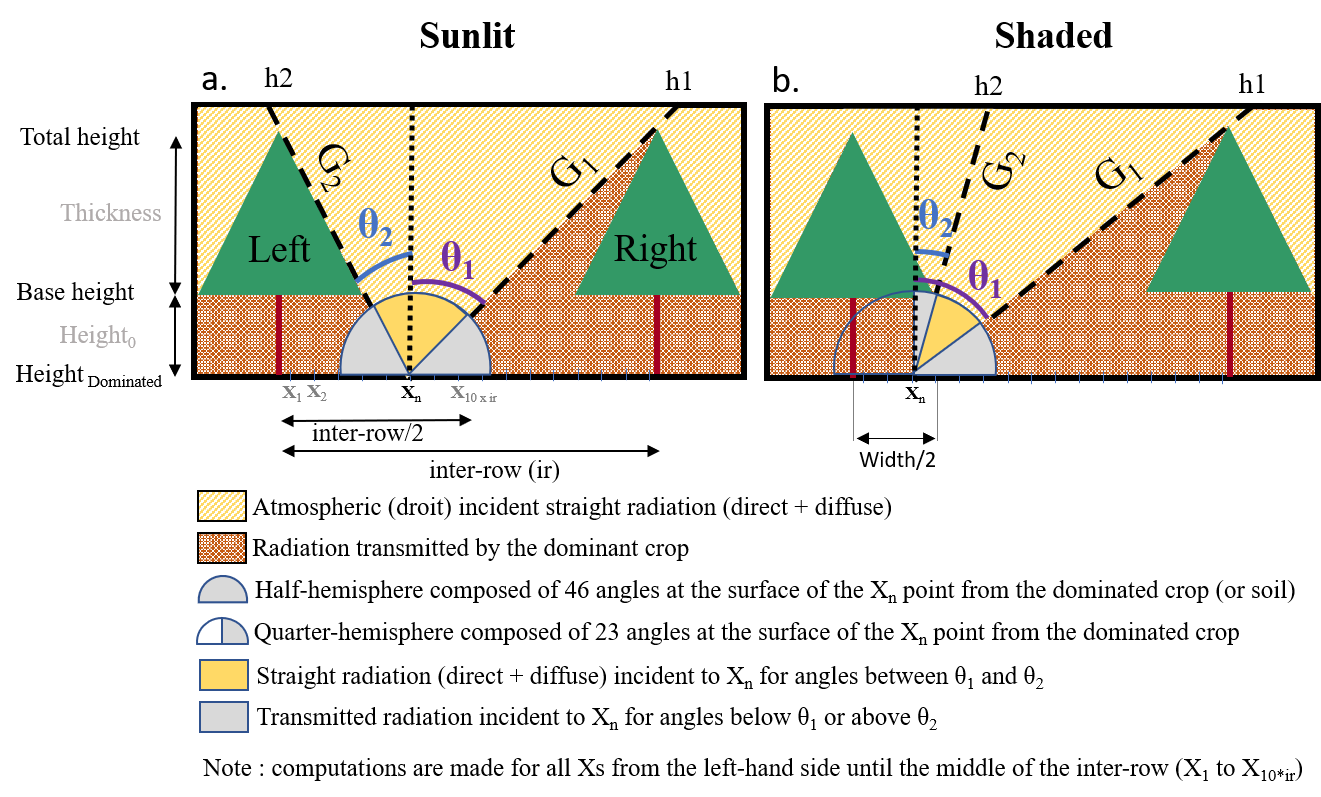
\includegraphics{img/Light-interception-dominated.png}
\caption{\label{fig:Compdominated}\textbf{Diagram of the computation workflow of STICS for radiation interception for two X points placed above the dominated plant species. a. The X point is considered sunlit; b. The X point is considered shaded (right under the dominant plant canopy), so only the right-hand side of the semi-hemisphere is computed for atmospheric radiation}}
\end{figure}

\hypertarget{incident-direct-radiation-from-the-atmosphere}{%
\subsection{Incident direct radiation from the atmosphere}\label{incident-direct-radiation-from-the-atmosphere}}

The incident direct radiation for each X point is computed for all angles of the hemisphere between \(\theta_1\) and \(\theta_2\) (see \ref{fig:Compdominated}), and summed up to integrate the semi-hemisphere of each point.

Here is an example of the computation of the direct proportion received at each X point for a crop using the \texttt{kgeom()} function:

\begin{Shaded}
\begin{Highlighting}[]
\NormalTok{decangle=}\StringTok{ }\ControlFlowTok{function}\NormalTok{(j)\{}
\NormalTok{  theta1 =}\StringTok{ }\DecValTok{2} \OperatorTok{*}\StringTok{ }\NormalTok{pi }\OperatorTok{*}\StringTok{ }\NormalTok{(j }\OperatorTok{-}\StringTok{ }\DecValTok{80}\NormalTok{) }\OperatorTok{/}\StringTok{ }\DecValTok{365}
\NormalTok{  theta2 =}\StringTok{ }\FloatTok{0.034} \OperatorTok{*}\StringTok{ }\NormalTok{(}\KeywordTok{sin}\NormalTok{(}\DecValTok{2} \OperatorTok{*}\StringTok{ }\NormalTok{pi }\OperatorTok{*}\StringTok{ }\NormalTok{j }\OperatorTok{/}\StringTok{ }\DecValTok{365}\NormalTok{) }\OperatorTok{-}\StringTok{ }\KeywordTok{sin}\NormalTok{(}\DecValTok{2} \OperatorTok{*}\StringTok{ }\NormalTok{pi }\OperatorTok{*}\StringTok{ }\DecValTok{80} \OperatorTok{/}\StringTok{ }\DecValTok{365}\NormalTok{))}
\NormalTok{  theta =}\StringTok{ }\NormalTok{theta1 }\OperatorTok{-}\StringTok{ }\NormalTok{theta2}
\NormalTok{  decangle =}\StringTok{ }\KeywordTok{asin}\NormalTok{(}\FloatTok{0.3978} \OperatorTok{*}\StringTok{ }\KeywordTok{sin}\NormalTok{(theta))}
\NormalTok{\}}

\NormalTok{thetacrit=}\StringTok{ }\ControlFlowTok{function}\NormalTok{(lat,j,tgh,alpha)\{}
  
\NormalTok{  acrit =}\StringTok{ }\FloatTok{0.0}
\NormalTok{  bcrit =}\StringTok{ }\FloatTok{0.0}
\NormalTok{  a =}\StringTok{ }\FloatTok{0.0}
\NormalTok{  b =}\StringTok{ }\FloatTok{0.0}
\NormalTok{  thetacr =}\StringTok{ }\FloatTok{0.0}
\NormalTok{  hcritprec=}\StringTok{ }\DecValTok{0}
\NormalTok{  n  =}\StringTok{ }\DecValTok{3}
\NormalTok{  dec =}\StringTok{ }\KeywordTok{decangle}\NormalTok{(j)}
\NormalTok{  hprec =}\StringTok{ }\FloatTok{0.0}
\NormalTok{  pi =}\StringTok{ }\DecValTok{4} \OperatorTok{*}\StringTok{ }\KeywordTok{atan}\NormalTok{(}\FloatTok{1.0}\NormalTok{)}
\NormalTok{  theta=}\StringTok{ }\KeywordTok{rep}\NormalTok{(}\DecValTok{0}\NormalTok{,}\DecValTok{180}\NormalTok{)}
  
  \ControlFlowTok{for}\NormalTok{(i }\ControlFlowTok{in} \DecValTok{1}\OperatorTok{:}\NormalTok{(}\DecValTok{18} \OperatorTok{*}\StringTok{ }\NormalTok{n))\{}
\NormalTok{    theta[i] =}\StringTok{ }\FloatTok{10.} \OperatorTok{/}\StringTok{ }\NormalTok{n }\OperatorTok{*}\StringTok{ }\NormalTok{(i }\OperatorTok{-}\StringTok{ }\DecValTok{1}\NormalTok{)}
\NormalTok{    theta[i] =}\StringTok{ }\NormalTok{(theta[i] }\OperatorTok{-}\StringTok{ }\DecValTok{90}\NormalTok{) }\OperatorTok{/}\StringTok{ }\DecValTok{180} \OperatorTok{*}\StringTok{ }\NormalTok{pi}
    \CommentTok{# Sun position (h,azim)}
\NormalTok{    sinh =}\StringTok{ }\KeywordTok{sin}\NormalTok{(lat) }\OperatorTok{*}\StringTok{ }\KeywordTok{sin}\NormalTok{(dec) }\OperatorTok{+}\StringTok{ }\KeywordTok{cos}\NormalTok{(lat) }\OperatorTok{*}\StringTok{ }\KeywordTok{cos}\NormalTok{(dec) }\OperatorTok{*}\StringTok{ }\KeywordTok{cos}\NormalTok{(theta[i])}
\NormalTok{    h =}\StringTok{ }\KeywordTok{asin}\NormalTok{(sinh)}
\NormalTok{    cosazim =}\StringTok{ }\NormalTok{(}\OperatorTok{-}\KeywordTok{cos}\NormalTok{(lat) }\OperatorTok{*}\StringTok{ }\KeywordTok{sin}\NormalTok{(dec) }\OperatorTok{+}\StringTok{ }\KeywordTok{sin}\NormalTok{(lat) }\OperatorTok{*}\StringTok{ }\KeywordTok{cos}\NormalTok{(dec) }\OperatorTok{*}\StringTok{ }\KeywordTok{cos}\NormalTok{(theta[i])) }\OperatorTok{/}\StringTok{ }\KeywordTok{cos}\NormalTok{(h)}
\NormalTok{    cosazim =}\StringTok{ }\KeywordTok{pmin}\NormalTok{(}\FloatTok{1.0}\NormalTok{,cosazim)}
    \ControlFlowTok{if}\NormalTok{(theta[i]}\OperatorTok{!=}\FloatTok{0.0}\NormalTok{)\{}
\NormalTok{      azim =}\StringTok{ }\KeywordTok{acos}\NormalTok{(cosazim) }\OperatorTok{*}\StringTok{ }\NormalTok{theta[i] }\OperatorTok{/}\StringTok{ }\KeywordTok{abs}\NormalTok{(theta[i])}
\NormalTok{    \}}\ControlFlowTok{else}\NormalTok{\{}
\NormalTok{      azim =}\StringTok{ }\FloatTok{0.0}
\NormalTok{    \}}
    \ControlFlowTok{if}\NormalTok{(sinh}\OperatorTok{<}\FloatTok{0.0}\NormalTok{)\{h =}\StringTok{ }\FloatTok{0.0}\NormalTok{\}}
    
    \CommentTok{# Critical height}
\NormalTok{    hcrit =}\StringTok{ }\KeywordTok{atan}\NormalTok{(tgh }\OperatorTok{*}\StringTok{ }\KeywordTok{abs}\NormalTok{(}\KeywordTok{sin}\NormalTok{(azim }\OperatorTok{+}\StringTok{ }\NormalTok{alpha }\OperatorTok{+}\StringTok{ }\FloatTok{0.00001}\NormalTok{)))}
    \CommentTok{# test for h = hcrit}
    \ControlFlowTok{if}\NormalTok{ (hcritprec }\OperatorTok{>=}\StringTok{ }\NormalTok{hprec }\OperatorTok{&}\StringTok{ }\NormalTok{hcrit }\OperatorTok{<=}\StringTok{ }\NormalTok{h }\OperatorTok{&}\StringTok{ }\NormalTok{i }\OperatorTok{>}\StringTok{ }\DecValTok{1}\NormalTok{)\{}
      \CommentTok{# Linear interpolation:}
\NormalTok{      acrit =}\StringTok{ }\NormalTok{(hcrit }\OperatorTok{-}\StringTok{ }\NormalTok{hcritprec) }\OperatorTok{/}\StringTok{ }\NormalTok{(theta[i] }\OperatorTok{-}\StringTok{ }\NormalTok{theta[i}\DecValTok{-1}\NormalTok{])}
\NormalTok{      bcrit =}\StringTok{ }\NormalTok{hcrit }\OperatorTok{-}\StringTok{ }\NormalTok{acrit }\OperatorTok{*}\StringTok{ }\NormalTok{theta[i]}
\NormalTok{      a =}\StringTok{ }\NormalTok{(h }\OperatorTok{-}\StringTok{ }\NormalTok{hprec) }\OperatorTok{/}\StringTok{ }\NormalTok{(theta[i] }\OperatorTok{-}\StringTok{ }\NormalTok{theta[i}\DecValTok{-1}\NormalTok{])}
\NormalTok{      b =}\StringTok{ }\NormalTok{h }\OperatorTok{-}\StringTok{ }\NormalTok{a }\OperatorTok{*}\StringTok{ }\NormalTok{theta[i]}
      
      \ControlFlowTok{if}\NormalTok{(a}\OperatorTok{!=}\NormalTok{acrit)\{thetacr =}\StringTok{ }\NormalTok{(b }\OperatorTok{-}\StringTok{ }\NormalTok{bcrit) }\OperatorTok{/}\StringTok{ }\NormalTok{(acrit }\OperatorTok{-}\StringTok{ }\NormalTok{a)\}}
\NormalTok{      hcritprec =}\StringTok{ }\NormalTok{hcrit}
\NormalTok{      hprec =}\StringTok{ }\NormalTok{h}
\NormalTok{    \}}
\NormalTok{  \}}
  \KeywordTok{return}\NormalTok{(thetacr)}
\NormalTok{\}}

\NormalTok{e =}\StringTok{ }\KeywordTok{abs}\NormalTok{(l }\OperatorTok{*}\StringTok{ }\NormalTok{rap) }\CommentTok{# Thickness of the plant crown}
\NormalTok{xprec=}\StringTok{ }\DecValTok{0}         \CommentTok{# Init.}
\NormalTok{limite =}\StringTok{ }\NormalTok{l }\OperatorTok{/}\StringTok{ }\DecValTok{2}

\ControlFlowTok{if}\NormalTok{(ir}\OperatorTok{<}\FloatTok{1.0}\NormalTok{)\{interval =}\StringTok{ }\FloatTok{200.}\NormalTok{\}}\ControlFlowTok{else}\NormalTok{\{interval =}\StringTok{ }\FloatTok{20.}\NormalTok{\}}
\ControlFlowTok{if}\NormalTok{(l}\OperatorTok{>}\NormalTok{ir}\OperatorTok{/}\FloatTok{2.}\NormalTok{)\{l =}\StringTok{ }\NormalTok{ir}\OperatorTok{/}\FloatTok{2.}\NormalTok{\}}

\ControlFlowTok{if}\NormalTok{(e}\OperatorTok{>}\FloatTok{0.0}\NormalTok{)\{}
\NormalTok{  limite2 =}\StringTok{ }\NormalTok{l}\OperatorTok{/}\DecValTok{2} \OperatorTok{*}\StringTok{ }\NormalTok{(haut}\OperatorTok{/}\NormalTok{e}\OperatorTok{+}\DecValTok{1}\NormalTok{)}
\NormalTok{\}}\ControlFlowTok{else}\NormalTok{\{}
\NormalTok{  P_forme =}\StringTok{ }\DecValTok{1}
\NormalTok{\}}
\CommentTok{# NB : is it sure that it is (haut/e+1) and not (haut/(e+1)) ? }

\CommentTok{# Saving some intermediate results for output here (not in the real function):}
\NormalTok{x_s=}\StringTok{ }\NormalTok{(}\DecValTok{1}\OperatorTok{:}\NormalTok{(ir }\OperatorTok{/}\StringTok{ }\DecValTok{2} \OperatorTok{*}\StringTok{ }\NormalTok{interval))}
\NormalTok{Output=}\StringTok{ }\KeywordTok{data.frame}\NormalTok{(}\DataTypeTok{x_index=}\NormalTok{ x_s,}
                   \DataTypeTok{x_value=}\NormalTok{ (x_s}\DecValTok{-1}\NormalTok{)}\OperatorTok{/}\NormalTok{interval,}
                   \DataTypeTok{theta1=} \KeywordTok{rep}\NormalTok{(}\OtherTok{NA_real_}\NormalTok{,}\KeywordTok{length}\NormalTok{(x_s)),}
                   \DataTypeTok{theta2=} \KeywordTok{rep}\NormalTok{(}\OtherTok{NA_real_}\NormalTok{,}\KeywordTok{length}\NormalTok{(x_s)),}
                   \DataTypeTok{theta1_deg=} \KeywordTok{rep}\NormalTok{(}\OtherTok{NA_real_}\NormalTok{,}\KeywordTok{length}\NormalTok{(x_s)),}
                   \DataTypeTok{theta2_deg=} \KeywordTok{rep}\NormalTok{(}\OtherTok{NA_real_}\NormalTok{,}\KeywordTok{length}\NormalTok{(x_s)),}
                   \DataTypeTok{kg=} \KeywordTok{rep}\NormalTok{(}\DecValTok{0}\NormalTok{,}\KeywordTok{length}\NormalTok{(x_s)))}

\CommentTok{# Loop over Xs:}

\ControlFlowTok{for}\NormalTok{(i }\ControlFlowTok{in}\NormalTok{ x_s)\{}
\NormalTok{  x =}\StringTok{ }\NormalTok{(i}\DecValTok{-1}\NormalTok{) }\OperatorTok{/}\StringTok{ }\NormalTok{interval}
  \ControlFlowTok{if}\NormalTok{(xprec}\OperatorTok{<=}\NormalTok{l}\OperatorTok{/}\DecValTok{2}\OperatorTok{&}\NormalTok{x}\OperatorTok{>=}\NormalTok{l}\OperatorTok{/}\DecValTok{2}\NormalTok{)\{ilim =}\StringTok{ }\NormalTok{i\}}
\NormalTok{  xprec =}\StringTok{ }\NormalTok{x}
  
  \CommentTok{# kdir:}
  
  \CommentTok{# Rectangle:}
  \ControlFlowTok{if}\NormalTok{(P_forme}\OperatorTok{==}\DecValTok{1}\NormalTok{)\{}
\NormalTok{    tgh1 =}\StringTok{ }\NormalTok{(haut }\OperatorTok{+}\StringTok{ }\NormalTok{e) }\OperatorTok{/}\StringTok{ }\NormalTok{(ir }\OperatorTok{-}\StringTok{ }\NormalTok{x }\OperatorTok{-}\StringTok{ }\NormalTok{limite)}
\NormalTok{    theta1 =}\StringTok{ }\KeywordTok{thetacrit}\NormalTok{(lat,j,tgh1,alpha)}
    \ControlFlowTok{if}\NormalTok{(x}\OperatorTok{>}\NormalTok{limite)\{}
\NormalTok{      tgh2 =}\StringTok{ }\NormalTok{(haut }\OperatorTok{+}\StringTok{ }\NormalTok{e) }\OperatorTok{/}\StringTok{ }\NormalTok{(x }\OperatorTok{-}\StringTok{ }\NormalTok{limite)}
\NormalTok{      theta2 =}\StringTok{ }\KeywordTok{thetacrit}\NormalTok{(lat,j,tgh2,alpha)}
\NormalTok{    \}}\ControlFlowTok{else} \ControlFlowTok{if}\NormalTok{(x }\OperatorTok{<}\StringTok{ }\NormalTok{limite)\{}
\NormalTok{      tgh2 =}\StringTok{ }\NormalTok{haut }\OperatorTok{/}\StringTok{ }\NormalTok{( }\OperatorTok{-}\NormalTok{x }\OperatorTok{+}\StringTok{ }\NormalTok{limite)}
\NormalTok{      theta2 =}\StringTok{ }\OperatorTok{-}\KeywordTok{thetacrit}\NormalTok{(lat,j,tgh2,alpha)}
\NormalTok{    \}}\ControlFlowTok{else}\NormalTok{\{}
      \CommentTok{# x == limite}
\NormalTok{      theta2 =}\StringTok{ }\DecValTok{0}
\NormalTok{    \}}
\NormalTok{  \}}
  
  \CommentTok{# Downside Triangle:}
  \ControlFlowTok{if}\NormalTok{ (P_forme}\OperatorTok{==}\DecValTok{2} \OperatorTok{&}\StringTok{ }\NormalTok{rap}\OperatorTok{<}\FloatTok{0.}\NormalTok{)\{}
\NormalTok{    tgh1 =}\StringTok{ }\NormalTok{(haut }\OperatorTok{+}\StringTok{ }\NormalTok{e) }\OperatorTok{/}\StringTok{ }\NormalTok{(ir }\OperatorTok{-}\StringTok{ }\NormalTok{x }\OperatorTok{-}\StringTok{ }\NormalTok{limite)}
\NormalTok{    theta1 =}\StringTok{ }\KeywordTok{thetacrit}\NormalTok{(lat,j,tgh1,alpha)}
    \ControlFlowTok{if}\NormalTok{ (x }\OperatorTok{>}\StringTok{ }\NormalTok{limite)\{}
\NormalTok{      tgh2 =}\StringTok{ }\NormalTok{(haut }\OperatorTok{+}\StringTok{ }\NormalTok{e) }\OperatorTok{/}\StringTok{ }\NormalTok{(x }\OperatorTok{-}\StringTok{ }\NormalTok{limite)}
\NormalTok{      theta2 =}\StringTok{ }\KeywordTok{thetacrit}\NormalTok{(lat,j,tgh2,alpha)}
\NormalTok{    \}}\ControlFlowTok{else} \ControlFlowTok{if}\NormalTok{(x }\OperatorTok{<}\StringTok{ }\NormalTok{limite)\{}
\NormalTok{      tgh2 =}\StringTok{ }\NormalTok{(haut }\OperatorTok{+}\StringTok{ }\NormalTok{e) }\OperatorTok{/}\StringTok{ }\NormalTok{( x }\OperatorTok{-}\StringTok{ }\NormalTok{limite)}
\NormalTok{      theta2 =}\StringTok{ }\OperatorTok{-}\KeywordTok{thetacrit}\NormalTok{(lat,j,tgh2,alpha)}
\NormalTok{    \}}\ControlFlowTok{else}\NormalTok{\{}
\NormalTok{      theta2 =}\StringTok{ }\DecValTok{0}
\NormalTok{    \}}
\NormalTok{  \}}
  
  \CommentTok{# Upside Triangle:}
  \ControlFlowTok{if}\NormalTok{ (P_forme}\OperatorTok{==}\DecValTok{2}\OperatorTok{&}\NormalTok{rap}\OperatorTok{>}\FloatTok{0.}\NormalTok{)\{ then}
\NormalTok{    tgh1 =}\StringTok{ }\NormalTok{(haut }\OperatorTok{+}\StringTok{ }\NormalTok{e) }\OperatorTok{/}\StringTok{ }\NormalTok{(ir }\OperatorTok{-}\StringTok{ }\NormalTok{x }\OperatorTok{-}\StringTok{ }\NormalTok{limite)}
\NormalTok{    theta1 =}\StringTok{ }\KeywordTok{thetacrit}\NormalTok{(lat,j,tgh1,alpha)}
    \ControlFlowTok{if}\NormalTok{ (x }\OperatorTok{<}\StringTok{ }\NormalTok{limite2)\{}
      \ControlFlowTok{if}\NormalTok{ (x }\OperatorTok{>}\StringTok{ }\NormalTok{limite)\{}
\NormalTok{        tgh2 =}\StringTok{ }\NormalTok{haut }\OperatorTok{/}\StringTok{ }\NormalTok{( x }\OperatorTok{-}\StringTok{ }\NormalTok{limite)}
\NormalTok{        theta2 =}\StringTok{ }\KeywordTok{thetacrit}\NormalTok{(lat,j,tgh2,alpha)}
\NormalTok{      \}}\ControlFlowTok{else} \ControlFlowTok{if}\NormalTok{(x }\OperatorTok{<}\StringTok{ }\NormalTok{limite)\{}
\NormalTok{        tgh2 =}\StringTok{ }\NormalTok{haut }\OperatorTok{/}\StringTok{ }\NormalTok{(limite }\OperatorTok{-}\StringTok{ }\NormalTok{x)}
\NormalTok{        theta2 =}\StringTok{ }\OperatorTok{-}\KeywordTok{thetacrit}\NormalTok{(lat,j,tgh2,alpha)}
\NormalTok{      \}}\ControlFlowTok{else}\NormalTok{\{}
\NormalTok{        theta2 =}\StringTok{ }\FloatTok{0.0}
\NormalTok{      \}}
\NormalTok{    \}}\ControlFlowTok{else} \ControlFlowTok{if}\NormalTok{(x }\OperatorTok{>=}\StringTok{ }\NormalTok{limite2)\{}
\NormalTok{      tgh2 =}\StringTok{ }\NormalTok{(haut }\OperatorTok{+}\StringTok{ }\NormalTok{e) }\OperatorTok{/}\StringTok{ }\NormalTok{x}
\NormalTok{      theta2 =}\StringTok{ }\KeywordTok{thetacrit}\NormalTok{(lat,j,tgh2,alpha)}
\NormalTok{    \}}
\NormalTok{  \}}
  
  \CommentTok{# NB: is there a missing else here ? kg is modified just after...}
  \ControlFlowTok{if}\NormalTok{(e }\OperatorTok{>}\StringTok{ }\FloatTok{2.1e-2}\NormalTok{)\{}
\NormalTok{    kg =}\StringTok{ }\KeywordTok{cos}\NormalTok{(theta1)}
\NormalTok{    kg =}\StringTok{ }\KeywordTok{cos}\NormalTok{(theta2)}
\NormalTok{  \}}
\NormalTok{  kg =}\StringTok{ }\FloatTok{0.5} \OperatorTok{*}\StringTok{ }\NormalTok{(}\KeywordTok{cos}\NormalTok{(pi}\OperatorTok{/}\DecValTok{2} \OperatorTok{+}\StringTok{ }\NormalTok{theta1) }\OperatorTok{+}\StringTok{ }\KeywordTok{cos}\NormalTok{(pi}\OperatorTok{/}\DecValTok{2} \OperatorTok{+}\StringTok{ }\NormalTok{theta2))}
\NormalTok{  kg =}\StringTok{ }\KeywordTok{max}\NormalTok{(kg,}\FloatTok{0.0}\NormalTok{)}
  
\NormalTok{  Output}\OperatorTok{$}\NormalTok{theta1[Output}\OperatorTok{$}\NormalTok{x_index}\OperatorTok{==}\NormalTok{i]=}\StringTok{ }\NormalTok{theta1}
\NormalTok{  Output}\OperatorTok{$}\NormalTok{theta2[Output}\OperatorTok{$}\NormalTok{x_index}\OperatorTok{==}\NormalTok{i]=}\StringTok{ }\NormalTok{theta2}
\NormalTok{  Output}\OperatorTok{$}\NormalTok{kg[Output}\OperatorTok{$}\NormalTok{x_index}\OperatorTok{==}\NormalTok{i]=}\StringTok{ }\NormalTok{kg}
\NormalTok{\}}

\NormalTok{Output}\OperatorTok{$}\NormalTok{theta1_deg=}\StringTok{ }\NormalTok{(pi}\OperatorTok{/}\DecValTok{2}\OperatorTok{+}\NormalTok{Output}\OperatorTok{$}\NormalTok{theta1)}\OperatorTok{*}\DecValTok{180}\OperatorTok{/}\NormalTok{pi}
\NormalTok{Output}\OperatorTok{$}\NormalTok{theta2_deg=}\StringTok{ }\NormalTok{(pi}\OperatorTok{/}\DecValTok{2}\OperatorTok{-}\NormalTok{Output}\OperatorTok{$}\NormalTok{theta2)}\OperatorTok{*}\DecValTok{180}\OperatorTok{/}\NormalTok{pi}

\KeywordTok{colnames}\NormalTok{(Output)=}\StringTok{ }\KeywordTok{c}\NormalTok{(}\StringTok{"X index"}\NormalTok{,}\StringTok{"X value (m)"}\NormalTok{,}\StringTok{"Theta 1 (rad)"}\NormalTok{,}\StringTok{"Theta 2 (rad)"}\NormalTok{,}
                    \StringTok{"Theta 1 (deg)"}\NormalTok{,}\StringTok{"Theta 2 (deg)"}\NormalTok{,}\StringTok{"kgdirect"}\NormalTok{)}

\KeywordTok{kable}\NormalTok{(Output, }\DataTypeTok{caption=} \KeywordTok{paste}\NormalTok{(}\StringTok{"Example of the computation of the incident direct"}\NormalTok{,}
                             \StringTok{"radiation ratio kgdirect. See introduction section"}\NormalTok{,}
                             \StringTok{"for further details on the crop."}\NormalTok{))}
\end{Highlighting}
\end{Shaded}

\begin{table}

\caption{\label{tab:kdir}Example of the computation of the incident direct radiation ratio kgdirect. See introduction section for further details on the crop.}
\centering
\begin{tabular}[t]{r|r|r|r|r|r|r}
\hline
X index & X value (m) & Theta 1 (rad) & Theta 2 (rad) & Theta 1 (deg) & Theta 2 (deg) & kgdirect\\
\hline
1 & 0.00 & -0.7563093 & 0.1163553 & 46.66667 & 83.33333 & 0.2850744\\
\hline
2 & 0.05 & -0.7563093 & 0.0581776 & 46.66667 & 86.66667 & 0.3140484\\
\hline
3 & 0.10 & -0.6981317 & 0.0000000 & 50.00000 & 90.00000 & 0.3213938\\
\hline
4 & 0.15 & -0.6981317 & -0.0581776 & 50.00000 & 93.33333 & 0.3504662\\
\hline
5 & 0.20 & -0.6399541 & -0.1163553 & 53.33333 & 96.66667 & 0.3566258\\
\hline
6 & 0.25 & -0.6399541 & -0.1745329 & 53.33333 & 100.00000 & 0.3854034\\
\hline
7 & 0.30 & -0.5817764 & -0.2327106 & 56.66667 & 103.33333 & 0.3900624\\
\hline
8 & 0.35 & -0.5235988 & -0.2908882 & 60.00000 & 106.66667 & 0.3934016\\
\hline
9 & 0.40 & -0.4654211 & -0.2908882 & 63.33333 & 106.66667 & 0.3678012\\
\hline
10 & 0.45 & -0.4654211 & -0.3490659 & 63.33333 & 110.00000 & 0.3954097\\
\hline
\end{tabular}
\end{table}

Where \(\theta_1\) and \(\theta_2\) are the angles visible in \protect\hyperlink{fig:Compdominated}{fig.3} and kgdirect the proportion of the semi-hemisphere that receive direct light, considering sun position throughout the day by using stand latitude, day of year and row orientation. In the model, \(\theta_1\) and \(\theta_2\) are computed in radian relative to the vertical plane above X. To provide a simpler representation, \(\theta_1\) and \(\theta_2\) are also given in degrees relative to the horizontal plane (i.e.~soil or dominated plant species surface) in tab.\ref{tab:kdir}.

\hypertarget{incident-diffuse-radiation-from-the-atmosphere}{%
\subsection{Incident diffuse radiation from the atmosphere}\label{incident-diffuse-radiation-from-the-atmosphere}}

The incident diffuse radiation for all angles between \(\theta_1\) and \(\theta_2\) is computed using \texttt{G}, the apparent tangent to the considered \(\theta\). First the model computes it for \(\theta_1\), and uses it as a threshold under which no diffuse radiation comes from the atmosphere because only transmitted radiation reaches this angle for the considered X point. Second, the model tests if the X point is below the target crop canopy, and if not it computes \texttt{G} for \(\theta_2\), and applies the same methodology, with \texttt{G} being the upper threshold this time. This method avoids computing the left-hand quarter of the hemisphere since it receives only transmitted light necessarily if it is under the targeted crop.

Here is an example of the computation of the diffuse proportion received at each X point for the same crop as above (interrow= 1 meter, width= 0.2 meter, thickness= 0.1 meter, height= 1 meter) using the \texttt{kdif()} function:

\begin{Shaded}
\begin{Highlighting}[]
\CommentTok{# Initializations:}
\NormalTok{htab=}\StringTok{ }\KeywordTok{c}\NormalTok{(}\FloatTok{9.23}\NormalTok{, }\FloatTok{9.23}\NormalTok{, }\FloatTok{9.23}\NormalTok{, }\FloatTok{9.23}\NormalTok{, }\FloatTok{9.23}\NormalTok{, }\FloatTok{10.81}\NormalTok{, }\FloatTok{10.81}\NormalTok{, }\FloatTok{26.57}\NormalTok{,}
        \FloatTok{26.57}\NormalTok{, }\FloatTok{26.57}\NormalTok{, }\FloatTok{31.08}\NormalTok{, }\FloatTok{31.08}\NormalTok{, }\FloatTok{31.08}\NormalTok{, }\FloatTok{31.08}\NormalTok{, }\FloatTok{31.08}\NormalTok{, }\FloatTok{47.41}\NormalTok{,}
        \FloatTok{47.41}\NormalTok{, }\FloatTok{47.41}\NormalTok{, }\FloatTok{52.62}\NormalTok{, }\FloatTok{52.62}\NormalTok{, }\FloatTok{69.16}\NormalTok{, }\FloatTok{69.16}\NormalTok{, }\FloatTok{69.16}\NormalTok{)}
\NormalTok{aztab=}\StringTok{ }\KeywordTok{c}\NormalTok{(}\FloatTok{12.23}\NormalTok{,}\FloatTok{59.77}\NormalTok{,}\FloatTok{84.23}\NormalTok{,}\FloatTok{131.77}\NormalTok{,}\FloatTok{156.23}\NormalTok{,}\DecValTok{36}\NormalTok{,}\DecValTok{108}\NormalTok{,}\DecValTok{0}\NormalTok{,}\DecValTok{72}\NormalTok{,}\DecValTok{144}\NormalTok{,}\FloatTok{23.27}\NormalTok{,}\FloatTok{48.73}\NormalTok{,}\FloatTok{95.27}\NormalTok{,}
         \FloatTok{120.73}\NormalTok{,}\FloatTok{167.27}\NormalTok{,}\DecValTok{0}\NormalTok{,}\DecValTok{72}\NormalTok{,}\DecValTok{144}\NormalTok{,}\DecValTok{36}\NormalTok{,}\DecValTok{108}\NormalTok{,}\DecValTok{0}\NormalTok{,}\DecValTok{72}\NormalTok{,}\DecValTok{144}\NormalTok{)}
\NormalTok{SOCtab=}\StringTok{ }\KeywordTok{c}\NormalTok{(}\FloatTok{0.0043}\NormalTok{, }\FloatTok{0.0043}\NormalTok{, }\FloatTok{0.0043}\NormalTok{, }\FloatTok{0.0043}\NormalTok{, }\FloatTok{0.0043}\NormalTok{, }\FloatTok{0.0055}\NormalTok{,}
          \FloatTok{0.0055}\NormalTok{, }\FloatTok{0.0140}\NormalTok{, }\FloatTok{0.0140}\NormalTok{, }\FloatTok{0.0140}\NormalTok{, }\FloatTok{0.0197}\NormalTok{, }\FloatTok{0.0197}\NormalTok{,}
          \FloatTok{0.0197}\NormalTok{, }\FloatTok{0.0197}\NormalTok{, }\FloatTok{0.0197}\NormalTok{, }\FloatTok{0.0336}\NormalTok{, }\FloatTok{0.0336}\NormalTok{, }\FloatTok{0.0336}\NormalTok{,}
          \FloatTok{0.0399}\NormalTok{, }\FloatTok{0.0399}\NormalTok{, }\FloatTok{0.0495}\NormalTok{, }\FloatTok{0.0495}\NormalTok{, }\FloatTok{0.0495}\NormalTok{)}
\NormalTok{xprec=}\StringTok{ }\DecValTok{0}

\ControlFlowTok{if}\NormalTok{(ir}\OperatorTok{<}\FloatTok{1.0}\NormalTok{)\{interval =}\StringTok{ }\FloatTok{200.}\NormalTok{\}}\ControlFlowTok{else}\NormalTok{\{interval =}\StringTok{ }\FloatTok{20.}\NormalTok{\}}
\ControlFlowTok{if}\NormalTok{(l}\OperatorTok{>}\NormalTok{ir}\OperatorTok{/}\FloatTok{2.}\NormalTok{)\{l =}\StringTok{ }\NormalTok{ir}\OperatorTok{/}\FloatTok{2.}\NormalTok{\}}

\CommentTok{# Saving some intermediate results for Output_diff here (not in the real function):}
\NormalTok{x_s=}\StringTok{ }\NormalTok{(}\DecValTok{1}\OperatorTok{:}\NormalTok{(ir }\OperatorTok{/}\StringTok{ }\DecValTok{2} \OperatorTok{*}\StringTok{ }\NormalTok{interval))}
\NormalTok{Output_diff=}\StringTok{ }\KeywordTok{data.frame}\NormalTok{(}\DataTypeTok{x_index=} \KeywordTok{rep}\NormalTok{(x_s,}\DataTypeTok{each=}\DecValTok{23}\NormalTok{),}
                   \DataTypeTok{x_value=} \KeywordTok{rep}\NormalTok{((x_s}\DecValTok{-1}\NormalTok{)}\OperatorTok{/}\NormalTok{interval,}\DataTypeTok{each=}\DecValTok{23}\NormalTok{),}
                   \DataTypeTok{Angle =} \KeywordTok{rep}\NormalTok{(}\DecValTok{1}\OperatorTok{:}\DecValTok{23}\NormalTok{, }\KeywordTok{length}\NormalTok{(x_s)),}
                   \DataTypeTok{G1=} \KeywordTok{rep}\NormalTok{(}\OtherTok{NA_real_}\NormalTok{,}\KeywordTok{length}\NormalTok{(x_s)}\OperatorTok{*}\DecValTok{23}\NormalTok{),}
                   \DataTypeTok{G2=} \KeywordTok{rep}\NormalTok{(}\OtherTok{NA_real_}\NormalTok{,}\KeywordTok{length}\NormalTok{(x_s)}\OperatorTok{*}\DecValTok{23}\NormalTok{),}
                   \DataTypeTok{hcrit=} \KeywordTok{rep}\NormalTok{(}\DecValTok{0}\NormalTok{,}\KeywordTok{length}\NormalTok{(x_s)}\OperatorTok{*}\DecValTok{23}\NormalTok{),}
                   \DataTypeTok{kgdiffus=} \KeywordTok{rep}\NormalTok{(}\DecValTok{0}\NormalTok{,}\KeywordTok{length}\NormalTok{(x_s)}\OperatorTok{*}\DecValTok{23}\NormalTok{))}


\CommentTok{# Loop over Xs:}

\ControlFlowTok{for}\NormalTok{(i }\ControlFlowTok{in}\NormalTok{ x_s)\{}
\NormalTok{  x =}\StringTok{ }\NormalTok{(i}\DecValTok{-1}\NormalTok{) }\OperatorTok{/}\StringTok{ }\NormalTok{interval}
  \ControlFlowTok{if}\NormalTok{(xprec}\OperatorTok{<=}\NormalTok{l}\OperatorTok{/}\DecValTok{2}\OperatorTok{&}\NormalTok{x}\OperatorTok{>=}\NormalTok{l}\OperatorTok{/}\DecValTok{2}\NormalTok{)\{ilim =}\StringTok{ }\NormalTok{i\}}
\NormalTok{  xprec =}\StringTok{ }\NormalTok{x}
  
  \CommentTok{# kdif:}
  
\NormalTok{  x =}\StringTok{ }\KeywordTok{min}\NormalTok{(x,ir}\OperatorTok{/}\DecValTok{2}\NormalTok{)}
\NormalTok{  e =}\StringTok{ }\KeywordTok{abs}\NormalTok{(l}\OperatorTok{*}\NormalTok{rap)}
\NormalTok{  kgdiffus =}\StringTok{ }\FloatTok{0.}
  
  \CommentTok{# Computing for the right-hand of the row:}
\NormalTok{  G1 =}\StringTok{ }\NormalTok{(haut}\OperatorTok{+}\NormalTok{e)}\OperatorTok{/}\NormalTok{(ir}\OperatorTok{-}\NormalTok{x}\OperatorTok{-}\NormalTok{l}\OperatorTok{/}\FloatTok{2.}\NormalTok{) }\CommentTok{# the apparent tangent h1}
  \ControlFlowTok{for}\NormalTok{(j }\ControlFlowTok{in} \DecValTok{1}\OperatorTok{:}\DecValTok{23}\NormalTok{)\{}
\NormalTok{    hcrit =}\StringTok{ }\KeywordTok{atan}\NormalTok{(G1}\OperatorTok{*}\KeywordTok{sin}\NormalTok{(aztab[j]}\OperatorTok{/}\DecValTok{180}\OperatorTok{*}\NormalTok{pi))}\OperatorTok{/}\NormalTok{pi}\OperatorTok{*}\DecValTok{180}
    \ControlFlowTok{if}\NormalTok{(hcrit}\OperatorTok{<}\NormalTok{htab[j])\{}
\NormalTok{      kgdiffus =}\StringTok{ }\NormalTok{kgdiffus}\OperatorTok{+}\NormalTok{SOCtab[j]}
      \CommentTok{######## Not in the real function ########}
\NormalTok{      Output_diff}\OperatorTok{$}\NormalTok{kgdiffus[Output_diff}\OperatorTok{$}\NormalTok{x_index}\OperatorTok{==}\NormalTok{i}\OperatorTok{&}\NormalTok{Output_diff}\OperatorTok{$}\NormalTok{Angle}\OperatorTok{==}\NormalTok{j]=}\StringTok{ }\NormalTok{SOCtab[j]}
      \CommentTok{##########################################}
\NormalTok{    \}}
    \CommentTok{######## Not in the real function ########}
\NormalTok{    Output_diff}\OperatorTok{$}\NormalTok{hcrit[Output_diff}\OperatorTok{$}\NormalTok{x_index}\OperatorTok{==}\NormalTok{i}\OperatorTok{&}\NormalTok{Output_diff}\OperatorTok{$}\NormalTok{Angle}\OperatorTok{==}\NormalTok{j]=}\StringTok{ }\NormalTok{hcrit}
\NormalTok{    Output_diff}\OperatorTok{$}\NormalTok{G1[Output_diff}\OperatorTok{$}\NormalTok{x_index}\OperatorTok{==}\NormalTok{i}\OperatorTok{&}\NormalTok{Output_diff}\OperatorTok{$}\NormalTok{Angle}\OperatorTok{==}\NormalTok{j]=}\StringTok{ }\NormalTok{G1}
    \CommentTok{##########################################}
\NormalTok{  \}}
  
  \CommentTok{# Computing for the left-hand row, if the point is not a shaded point:}
  \ControlFlowTok{if}\NormalTok{(x}\OperatorTok{>}\NormalTok{l}\OperatorTok{/}\DecValTok{2}\NormalTok{)\{}
\NormalTok{    G2 =}\StringTok{ }\NormalTok{(haut}\OperatorTok{+}\NormalTok{e)}\OperatorTok{/}\NormalTok{(x}\OperatorTok{-}\NormalTok{l}\OperatorTok{/}\DecValTok{2}\NormalTok{) }\CommentTok{# the apparent tangent h2}
    \ControlFlowTok{for}\NormalTok{(j }\ControlFlowTok{in} \DecValTok{1}\OperatorTok{:}\DecValTok{23}\NormalTok{)\{}
\NormalTok{      hcrit =}\StringTok{ }\KeywordTok{atan}\NormalTok{(G2}\OperatorTok{*}\KeywordTok{sin}\NormalTok{(aztab[j]}\OperatorTok{/}\DecValTok{180}\OperatorTok{*}\NormalTok{pi))}\OperatorTok{/}\NormalTok{pi}\OperatorTok{*}\DecValTok{180}
      \ControlFlowTok{if}\NormalTok{(hcrit }\OperatorTok{<}\StringTok{ }\NormalTok{htab[j])\{}
\NormalTok{        kgdiffus =}\StringTok{ }\NormalTok{kgdiffus}\OperatorTok{+}\NormalTok{SOCtab[j]}
        \CommentTok{######## Not in the real function ########}
\NormalTok{        Output_diff}\OperatorTok{$}\NormalTok{kgdiffus[Output_diff}\OperatorTok{$}\NormalTok{x_index}\OperatorTok{==}\NormalTok{i}\OperatorTok{&}\NormalTok{Output_diff}\OperatorTok{$}\NormalTok{Angle}\OperatorTok{==}\NormalTok{j]=}\StringTok{ }
\StringTok{          }\NormalTok{Output_diff}\OperatorTok{$}\NormalTok{kgdiffus[Output_diff}\OperatorTok{$}\NormalTok{x_index}\OperatorTok{==}\NormalTok{i}\OperatorTok{&}\NormalTok{Output_diff}\OperatorTok{$}\NormalTok{Angle}\OperatorTok{==}\NormalTok{j]}\OperatorTok{+}\NormalTok{SOCtab[j]}
        \CommentTok{##########################################}
\NormalTok{      \}}
      \CommentTok{######## Not in the real function ########}
\NormalTok{      Output_diff}\OperatorTok{$}\NormalTok{hcrit[Output_diff}\OperatorTok{$}\NormalTok{x_index}\OperatorTok{==}\NormalTok{i}\OperatorTok{&}\NormalTok{Output_diff}\OperatorTok{$}\NormalTok{Angle}\OperatorTok{==}\NormalTok{j]=}\StringTok{ }\NormalTok{hcrit}
\NormalTok{      Output_diff}\OperatorTok{$}\NormalTok{G2[Output_diff}\OperatorTok{$}\NormalTok{x_index}\OperatorTok{==}\NormalTok{i}\OperatorTok{&}\NormalTok{Output_diff}\OperatorTok{$}\NormalTok{Angle}\OperatorTok{==}\NormalTok{j]=}\StringTok{ }\NormalTok{G2}
      \CommentTok{##########################################}
\NormalTok{    \}}
\NormalTok{  \}}
\NormalTok{\}}

\KeywordTok{colnames}\NormalTok{(Output_diff)=}\StringTok{ }\KeywordTok{c}\NormalTok{(}\StringTok{"X index"}\NormalTok{,}\StringTok{"X value (m)"}\NormalTok{,}\StringTok{"angle"}\NormalTok{,}\StringTok{"G1 (tangent)"}\NormalTok{,}
                         \StringTok{"G2 (tangent)"}\NormalTok{,}\StringTok{"hcrit"}\NormalTok{,}\StringTok{"kgdiffus"}\NormalTok{)}
\ControlFlowTok{if}\NormalTok{(knitr}\OperatorTok{:::}\KeywordTok{pandoc_to}\NormalTok{() }\OperatorTok{==}\StringTok{ "html"}\NormalTok{) \{Output_diff\}}\ControlFlowTok{else}\NormalTok{\{}
  \KeywordTok{kable}\NormalTok{(Output_diff[}\DecValTok{1}\OperatorTok{:}\DecValTok{10}\NormalTok{,],}
        \DataTypeTok{caption =} \KeywordTok{paste}\NormalTok{(}\StringTok{"Computation of the diffuse light incident on each"}\NormalTok{,}
                        \StringTok{"point x. Ten first rows only, for the full data,"}\NormalTok{,}
                        \StringTok{"please refer to the html version of this book"}\NormalTok{),}
        \DataTypeTok{col.names =} \KeywordTok{c}\NormalTok{(}\StringTok{"X index"}\NormalTok{,}\StringTok{"X value (m)"}\NormalTok{,}\StringTok{"angle"}\NormalTok{,}\StringTok{"G1 (tangent)"}\NormalTok{,}
                      \StringTok{"G2 (tangent)"}\NormalTok{,}\StringTok{"hcrit"}\NormalTok{,}\StringTok{"kgdiffus"}\NormalTok{), }\DataTypeTok{longtable =} \OtherTok{TRUE}\NormalTok{)}
\NormalTok{\}}
\end{Highlighting}
\end{Shaded}

\begin{longtable}[t]{r|r|r|r|r|r|r}
\caption{\label{tab:kdiff}Computation of the diffuse light incident on each point x. Ten first rows only, for the full data, please refer to the html version of this book}\\
\hline
X index & X value (m) & angle & G1 (tangent) & G2 (tangent) & hcrit & kgdiffus\\
\hline
1 & 0 & 1 & 1.222222 & NA & 14.51577 & 0.000\\
\hline
1 & 0 & 2 & 1.222222 & NA & 46.56057 & 0.000\\
\hline
1 & 0 & 3 & 1.222222 & NA & 50.56789 & 0.000\\
\hline
1 & 0 & 4 & 1.222222 & NA & 42.35117 & 0.000\\
\hline
1 & 0 & 5 & 1.222222 & NA & 26.22654 & 0.000\\
\hline
1 & 0 & 6 & 1.222222 & NA & 35.69363 & 0.000\\
\hline
1 & 0 & 7 & 1.222222 & NA & 49.29501 & 0.000\\
\hline
1 & 0 & 8 & 1.222222 & NA & 0.00000 & 0.014\\
\hline
1 & 0 & 9 & 1.222222 & NA & 49.29501 & 0.000\\
\hline
1 & 0 & 10 & 1.222222 & NA & 35.69363 & 0.000\\
\hline
\end{longtable}

The total diffuse radiation incident to each point X is simply the cumulative of each angle:

\begin{Shaded}
\begin{Highlighting}[]
\KeywordTok{suppressWarnings}\NormalTok{(}\KeywordTok{suppressPackageStartupMessages}\NormalTok{(}\KeywordTok{library}\NormalTok{(dplyr)))}
\NormalTok{Output_diff}\OperatorTok
\StringTok{  }\KeywordTok{group_by}\NormalTok{(}\StringTok{`}\DataTypeTok{X index}\StringTok{`}\NormalTok{)}\OperatorTok
\StringTok{  }\KeywordTok{summarise}\NormalTok{(}\DataTypeTok{kgdiffus=} \KeywordTok{sum}\NormalTok{(kgdiffus))}

\KeywordTok{kable}\NormalTok{(Output_diff,}\DataTypeTok{caption=} \KeywordTok{paste}\NormalTok{(}\StringTok{"Example of the computation of the incident diffuse"}\NormalTok{,}
\StringTok{"radiation ratio kgdiffus. See introduction section for further details on the crop."}\NormalTok{))}
\end{Highlighting}
\end{Shaded}

\begin{table}

\caption{\label{tab:kdifftot}Example of the computation of the incident diffuse radiation ratio kgdiffus. See introduction section for further details on the crop.}
\centering
\begin{tabular}[t]{r|r}
\hline
X index & kgdiffus\\
\hline
1 & 0.3489\\
\hline
2 & 0.3489\\
\hline
3 & 0.3489\\
\hline
4 & 0.4061\\
\hline
5 & 0.3864\\
\hline
6 & 0.3864\\
\hline
7 & 0.3864\\
\hline
8 & 0.4023\\
\hline
9 & 0.4023\\
\hline
10 & 0.3624\\
\hline
\end{tabular}
\end{table}

\hypertarget{total-diffuse-and-direct-radiation-from-the-atmosphere-incident-to-each-x-point}{%
\subsection{Total diffuse and direct radiation from the atmosphere incident to each X point}\label{total-diffuse-and-direct-radiation-from-the-atmosphere-incident-to-each-x-point}}

The total radiation from the atmosphere incident to each X point is computed by using the incident diffuse (\texttt{rdif}) and direct (\texttt{rdirect}) radiation coming from the atmosphere weighted respectively by the previously computed \texttt{kgdiffus} and \texttt{kgdirect} as follow:
\(rdroit=(kgdiffus\cdot rdif)+(kgdirect\cdot rdirect)\)

\hypertarget{light-tramsitted-by-the-dominant-crop-to-the-x-points}{%
\subsection{Light tramsitted by the dominant crop to the X points}\label{light-tramsitted-by-the-dominant-crop-to-the-x-points}}

The light transmitted by the dominant crop to the dominated crop (\texttt{rtransmis}) is computed using the total radiation from the atmosphere incident to each X point (\texttt{rdroit}) and the effective targeted plant leaf area index as follow:

\(rtransmis=(1.0-rdroit)\cdot e^{-P_{ktrou}\cdot(lai+eai)}\)

where \(P_{ktrou}\) is the targeted plant light extinction coefficient, \texttt{lai} the plant leaf area index, and \texttt{eai} the equivalent leaf area index, which represent the photosynthetic surface that is not from leaves (e.g.~wheat ears, rapeseed pods, pea pods or grapes during their green stage).

\hypertarget{total-light-incident-to-x-points}{%
\subsection{Total light incident to X points}\label{total-light-incident-to-x-points}}

The total light incident to each X point is the sum of the three components: atmospheric diffuse light, atmospheric direct light and transmitted light by the dominant crop.
Taking our previous example again, this computation leads to:

\begin{Shaded}
\begin{Highlighting}[]
\NormalTok{rdirect=}\StringTok{ }\DecValTok{1}\OperatorTok{-}\NormalTok{rdif}
\NormalTok{rdroit=}\StringTok{ }\NormalTok{(Output_diff}\OperatorTok{$}\NormalTok{kgdiffus}\OperatorTok{*}\NormalTok{rdif)}\OperatorTok{+}\NormalTok{(Output}\OperatorTok{$}\NormalTok{kg}\OperatorTok{*}\NormalTok{rdirect)}
\NormalTok{rtransmis =}\StringTok{ }\NormalTok{(}\FloatTok{1.0} \OperatorTok{-}\StringTok{ }\NormalTok{rdroit) }\OperatorTok{*}\StringTok{ }\NormalTok{(}\KeywordTok{exp}\NormalTok{(}\OperatorTok{-}\NormalTok{P_ktrou }\OperatorTok{*}\StringTok{ }\NormalTok{(lai }\OperatorTok{+}\StringTok{ }\NormalTok{eai)))}

\NormalTok{incident_light=}\StringTok{ }
\StringTok{  }\KeywordTok{data.frame}\NormalTok{(Output[,}\DecValTok{1}\OperatorTok{:}\DecValTok{2}\NormalTok{],}\DataTypeTok{Total=}\NormalTok{rdroit}\OperatorTok{+}\NormalTok{rtransmis, }\DataTypeTok{rdroit=}\NormalTok{ rdroit,}
             \DataTypeTok{rtransmis=}\NormalTok{ rtransmis, }
             \DataTypeTok{light_env=} \KeywordTok{ifelse}\NormalTok{(Output}\OperatorTok{$}\StringTok{`}\DataTypeTok{X value (m)}\StringTok{`}\OperatorTok{<}\NormalTok{limite,}\StringTok{"Shaded"}\NormalTok{,}\StringTok{"Sunlit"}\NormalTok{))}
\KeywordTok{kable}\NormalTok{(incident_light,}
      \DataTypeTok{col.names =} \KeywordTok{c}\NormalTok{(}\StringTok{"X index"}\NormalTok{,}\StringTok{"X value (m)"}\NormalTok{,}\StringTok{"Total incident ratio"}\NormalTok{,}
                    \StringTok{"Atmospheric ratio (rdroit)"}\NormalTok{,}\StringTok{"Transmitted ratio (rtransmis)"}\NormalTok{,}
                    \StringTok{"Light environment"}\NormalTok{),}
  \DataTypeTok{caption=}\KeywordTok{paste}\NormalTok{(}\StringTok{"Example of the computation of the total incident radiation ratio."}\NormalTok{,}
                \StringTok{"See introduction section for further details on the crop."}\NormalTok{))}
\end{Highlighting}
\end{Shaded}

\begin{table}

\caption{\label{tab:unnamed-chunk-5}Example of the computation of the total incident radiation ratio. See introduction section for further details on the crop.}
\centering
\begin{tabular}[t]{r|r|r|r|r|l}
\hline
X index & X value (m) & Total incident ratio & Atmospheric ratio (rdroit) & Transmitted ratio (rtransmis) & Light environment\\
\hline
1 & 0.00 & 0.3387059 & 0.3106046 & 0.0281013 & Shaded\\
\hline
2 & 0.05 & 0.3553817 & 0.3279890 & 0.0273926 & Shaded\\
\hline
3 & 0.10 & 0.3596093 & 0.3323963 & 0.0272130 & Sunlit\\
\hline
4 & 0.15 & 0.3982891 & 0.3727197 & 0.0255693 & Sunlit\\
\hline
5 & 0.20 & 0.3942753 & 0.3685355 & 0.0257399 & Sunlit\\
\hline
6 & 0.25 & 0.4108381 & 0.3858020 & 0.0250361 & Sunlit\\
\hline
7 & 0.30 & 0.4135196 & 0.3885975 & 0.0249221 & Sunlit\\
\hline
8 & 0.35 & 0.4215422 & 0.3969610 & 0.0245812 & Sunlit\\
\hline
9 & 0.40 & 0.4068080 & 0.3816007 & 0.0252073 & Sunlit\\
\hline
10 & 0.45 & 0.4073885 & 0.3822058 & 0.0251827 & Sunlit\\
\hline
\end{tabular}
\end{table}

The Total incident ratio is computed as: \texttt{Total\ incident\ ratio=\ rdroit+rtransmis}. It is the proportion of the incident ligth from the atmosphere that reach the point on the plane below the plant canopy. This light either comes directly from the sky (\texttt{rdroit}) or passing through the plant canopy (\texttt{rtransmis}).
Consequently, the first point \texttt{X} of our example that is right under the plant canopy receives in average 33.8705892\% of the light coming from the atmosphere: 31.0604617\% of the light directly from the sky (either direct or diffuse light) + 2.8101275\% of the light that is transmitted by the plant above.

\hypertarget{total-radiation-incident-to-the-plane}{%
\subsection{Total radiation incident to the plane}\label{total-radiation-incident-to-the-plane}}

After computing the total incident ratio for each point, the model averages the values between the so-called sunlit and shaded components. Each point positioned right under the plant canopy is considered shaded, and all other is considered sunlit (see fig.~\ref{fig:Compdominated}). using our previous example, this computation gives:

\begin{Shaded}
\begin{Highlighting}[]
\NormalTok{incident_light}\OperatorTok
\StringTok{  }\KeywordTok{group_by}\NormalTok{(light_env)}\OperatorTok
\StringTok{  }\KeywordTok{summarise}\NormalTok{(}\DataTypeTok{Total=} \KeywordTok{mean}\NormalTok{(Total))}\OperatorTok
\StringTok{  }\KeywordTok{transmute}\NormalTok{(}\DataTypeTok{Variable=} \KeywordTok{c}\NormalTok{(}\StringTok{"rombre"}\NormalTok{,}\StringTok{"rsoleil"}\NormalTok{),light_env,Total)}

\KeywordTok{kable}\NormalTok{(incident_light, }
      \DataTypeTok{col.names =} \KeywordTok{c}\NormalTok{(}\StringTok{"STICS variable name"}\NormalTok{,}\StringTok{"Light environment"}\NormalTok{,}
                    \StringTok{"Total incident light ratio"}\NormalTok{),}
      \DataTypeTok{caption=} \KeywordTok{paste}\NormalTok{(}\StringTok{"Example of the computation of the total incident radiation"}\NormalTok{,}
                     \StringTok{"ratio for each light environment for a horizontal plane below"}\NormalTok{,}
                     \StringTok{"the targeted plant canopy. See introduction section for further"}\NormalTok{,}
                     \StringTok{"details on the crop."}\NormalTok{))}
\end{Highlighting}
\end{Shaded}

\begin{table}

\caption{\label{tab:unnamed-chunk-6}Example of the computation of the total incident radiation ratio for each light environment for a horizontal plane below the targeted plant canopy. See introduction section for further details on the crop.}
\centering
\begin{tabular}[t]{l|l|r}
\hline
STICS variable name & Light environment & Total incident light ratio\\
\hline
rombre & Shaded & 0.3470438\\
\hline
rsoleil & Sunlit & 0.4015338\\
\hline
\end{tabular}
\end{table}

Finally, both ratios are used to compute the intercepted PAR \texttt{raint} (MJ m-2 d-1) of the target plant as:\\
\(raint=P_{parsurrg}\cdot trg\cdot(1-(rombre\cdot surfAO)-(rsoleil\cdot surfAS))\)\\
where \(P_{parsurrg}\) is a coefficient to compute PAR (Photosynthetically Active Radiation) from the global radiation, \texttt{trg} is the active radiation (either global radiation or radiation transmitted below the dominant crop), \texttt{rombre} and \texttt{rsoleil} are the ratio of incident light for shaded and sunlit components of the plane, and \texttt{surfAO} and \texttt{surfAS} are the relative surfaces (0 to 1) of the shaded and sunlit components of the plane.
The computation of \texttt{trg} is further described in Chapter \ref{trg}.

\begin{Shaded}
\begin{Highlighting}[]
\KeywordTok{library}\NormalTok{(tidyverse)}
\KeywordTok{library}\NormalTok{(magrittr)}
\NormalTok{P_parsurrg=}\StringTok{ }\FloatTok{0.5}
\NormalTok{incident_light}\OperatorTok\KeywordTok{spread}\NormalTok{(light_env,Total)}
\NormalTok{surfAO =}\StringTok{ }\NormalTok{l}\OperatorTok{/}\NormalTok{ir}
\NormalTok{surfAO =}\StringTok{ }\KeywordTok{min}\NormalTok{(surfAO,}\FloatTok{1.0}\NormalTok{)}
\NormalTok{surfAS =}\StringTok{ }\FloatTok{1.0} \OperatorTok{-}\StringTok{ }\NormalTok{surfAO}
\NormalTok{raint =}\StringTok{ }\NormalTok{P_parsurrg }\OperatorTok{*}\StringTok{ }\NormalTok{trg }\OperatorTok{*}\StringTok{ }\NormalTok{(}\DecValTok{1} \OperatorTok{-}\StringTok{ }\NormalTok{(incident_light}\OperatorTok{$}\NormalTok{Shaded[}\DecValTok{1}\NormalTok{] }\OperatorTok{*}\StringTok{ }\NormalTok{surfAO) }\OperatorTok{-}\StringTok{ }
\StringTok{                              }\NormalTok{(incident_light}\OperatorTok{$}\NormalTok{Sunlit[}\DecValTok{2}\NormalTok{]}\OperatorTok{*}\StringTok{ }\NormalTok{surfAS))}
\end{Highlighting}
\end{Shaded}

For our example, the crop would have intercepted 7.62 MJ m-2 day-1 of radiation, with a PAR of 12.5 W m-2, an \texttt{rombre} of 0.3470438, an \texttt{rsoleil} of 0.4015338 and a relative surface of 0.2 and 0.8 for the shaded and sunlit component respectively.

\begin{quote}
The relative surfaces (0 to 1) of the shaded and sunlit components of the plane (\texttt{surfAO} and \texttt{surfAS}) that are computed during the dominant plant computation are then used as the shaded and sunlit surfaces for the dominated plant.
\end{quote}

\hypertarget{summary}{%
\section{Summary}\label{summary}}

The interception of the targeted plant is obtained by:

\begin{enumerate}
\def\labelenumi{\arabic{enumi}.}
\tightlist
\item
  Computing the light that is incident at a horizontal plane at the height of the dominated plant (or the soil) and,
\item
  Substracting this incident light to the global PAR, which gives the PAR intercepted by the target plant.
\end{enumerate}

This process is applied iteratively to the dominant and the dominated plant to compute both species PAR interception while taking account for their respective structure (shape, height, width\ldots).

\hypertarget{discussion-and-proposed-modifications}{%
\section{Discussion and proposed modifications}\label{discussion-and-proposed-modifications}}

The dominated plant interception is computed in two separate computations, one for the sunlit component, and one for the shaded component, and interception is then weighted by their relative surface. The dominant plant is considered having 100\% of its surface that is sunlit, so all this computation is made only for its sunlit part.

The radiation above the dominant plant (\texttt{trg}) is the global radiation, but the radiation above the dominated plant (also \texttt{trg}) is computed as:
\(trg=trg\cdot rsoleil\)

where \texttt{rsoleil} is the average proportion of light intercepted by the sunlit area of the plane below the dominant plant.

This computation is only right for the sunlit component of the dominated plant. A modification is proposed, discussed and tested on Chapter \ref{trg}.

\hypertarget{trg}{%
\chapter{Light incident to the dominated crop (trg)}\label{trg}}

\hypertarget{computing-the-trg-incident-to-the-dominated-plant}{%
\section{Computing the trg incident to the dominated plant}\label{computing-the-trg-incident-to-the-dominated-plant}}

For the moment, STICS compute the radiation incident above the dominated (or associated) plant as:

Which means that trg for the dominated plant (\texttt{i\ \textgreater{}\ 1}) is computed as the global atmospheric radiation (\texttt{trg\_bak} here), reduced by the average proportion of light transmitted by the sunlit area of the plane below the dominant plant (and above the dominated plant).
This computation does not consider that the average proportion of light incident above the shaded part of the dominated plant (\texttt{rombre}) is different from \texttt{rsoleil}. See Chapter \ref{Light} for more details.

\hypertarget{proposed-solution}{%
\section{Proposed solution}\label{proposed-solution}}

We propose to change this computation to take the relevant incident light according to the light regime of the dominated plant under computation:

With this new computation, the radiation incident above the dominated plant depends from the component under consideration (shaded or sunlit), and is computed using the geometry of the dominant plant (for atmospheric+transmitted light computation).

\hypertarget{results}{%
\section{Results}\label{results}}

A comparison of the two was made using the \href{https://github.com/VEZY/sticRs}{sticRs} package, from which a summary plot was extracted. The results are shown in Figure \ref{fig:trgcomparison1}.

\begin{figure}
\centering
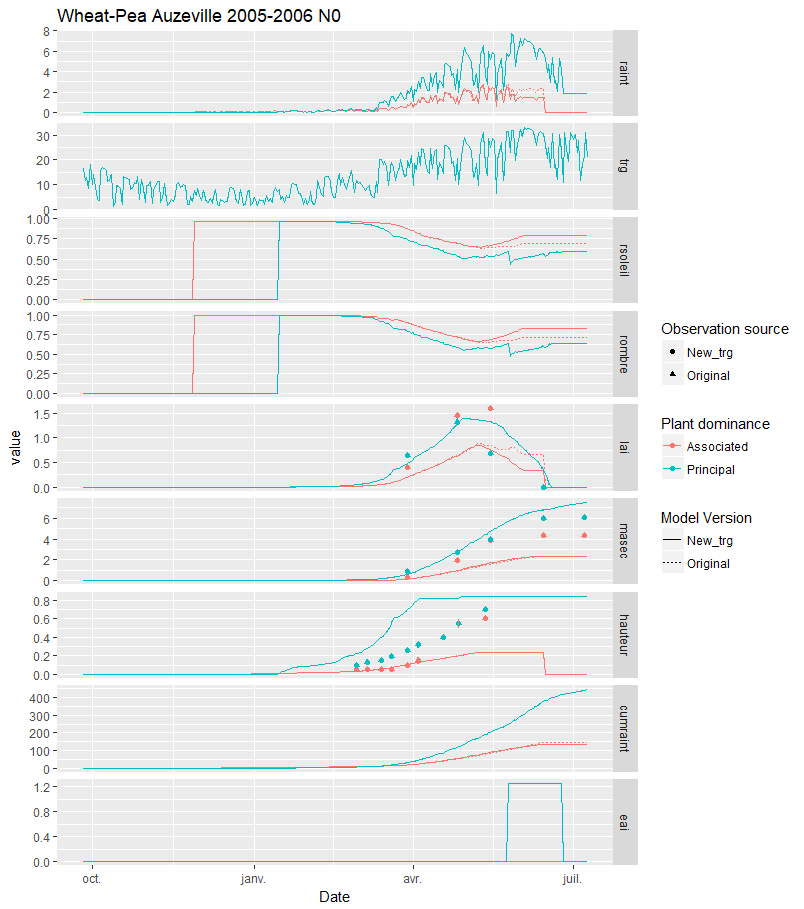
\includegraphics{img/trg-computation.png}
\caption{\label{fig:trgcomparison1}trg comparison}
\end{figure}

The comparison between both indicated that the dominated plant intercepted more PAR with the original computation (\texttt{raint}), due to its wrong light regime (\texttt{rsoleil} for both AS and AO). While the dry mass and height of the dominated plant did not change, its \texttt{LAI} was previously higher on the end of the rotation, which increased the \texttt{rsoleil} and \texttt{rombre} of the ground (visible as associated ones).
These simulations also showed that the wheat (dominant) \texttt{eai} was highly overestimated, which will be fixed in the next simulations.

\hypertarget{eai}{%
\chapter{Wheat EAI parameterization}\label{eai}}

\hypertarget{introduction-1}{%
\section{Introduction}\label{introduction-1}}

The simulations outputs from Chapter \ref{trg} have shown that the wheat ears equivalent photosynthetic surface area (\texttt{eai}) was probably overestimated by a 3-4 factor. This surface is computed using the fruit dry mass (\texttt{maenfruit}) and a parameter (\texttt{P\_sea}) as follow:

\(eai=P_{sea}\cdot\frac{maenfruit}{100}\)

This parameter was originally equal to 100, meaning that each gram of fruit dry mass gave 1 m2 of equivalent \texttt{LAI}. This value was probably overestimated, but before re-parameterizing the plant, we first needed to know the model sensitivity to this parameter.

\hypertarget{model-sensitivity-to-the-p_sea-parameter}{%
\section{\texorpdfstring{Model sensitivity to the \texttt{P\_sea} parameter}{Model sensitivity to the P\_sea parameter}}\label{model-sensitivity-to-the-p_sea-parameter}}

The model sensitivity was assessed using the \href{https://github.com/VEZY/sticRs}{sticRs} package using values from 10 to 90 for the \texttt{P\_sea} parameter. The results are shown below (see \texttt{html} version of this book for interactivity):

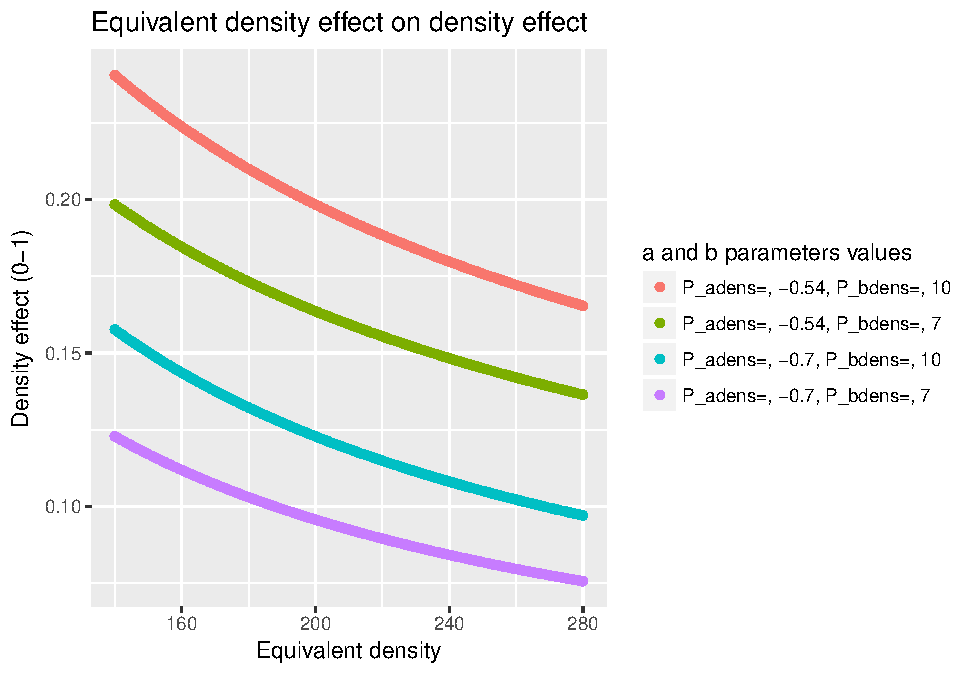
\includegraphics{Postdoc_steps_files/figure-latex/unnamed-chunk-12-1.pdf}

The results show that the higher the \texttt{P\_sea}, the higher the \texttt{eai}, and hence increasing the light interception (\texttt{raint}), which induced a higher aboveground dry mass (\texttt{masec}). The plant \texttt{LAI} is not influenced by the \texttt{P\_sea} though, because there is no retroactions on this variable.

In the case of intercrops, the \texttt{P\_sea} parameter can influence the dominated plant also, because less light is transmitted when \texttt{P\_sea} is high :

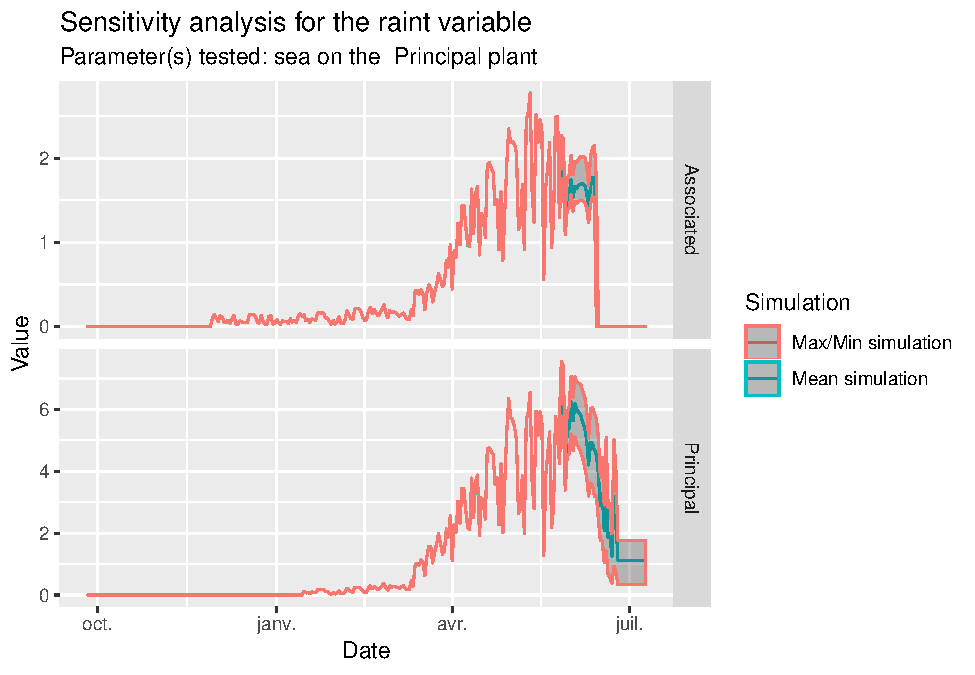
\includegraphics{Postdoc_steps_files/figure-latex/unnamed-chunk-13-1.pdf}

The other variables are not much impacted though:

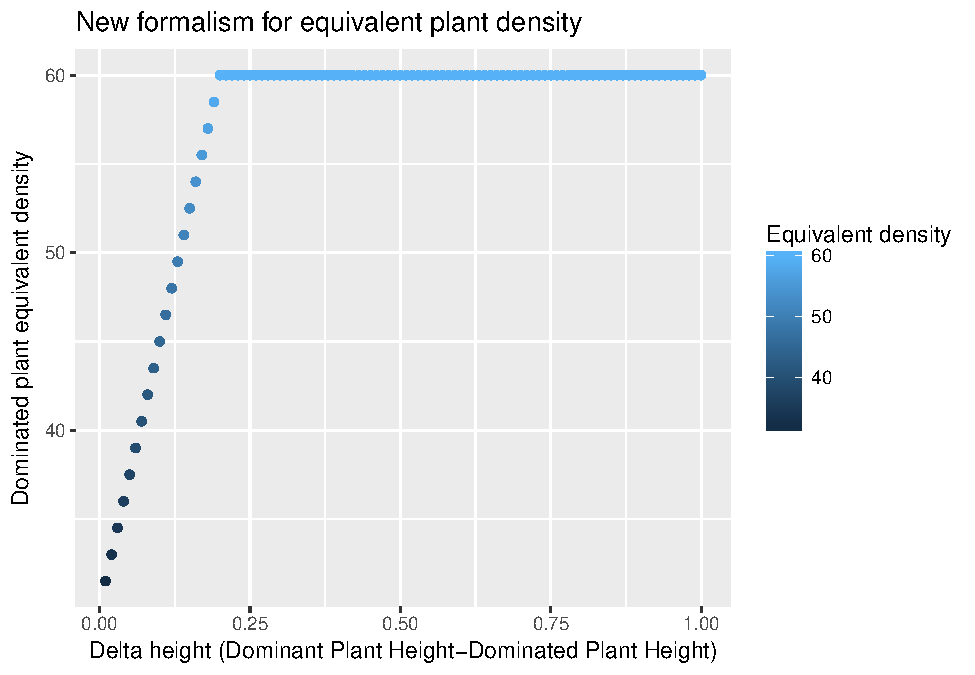
\includegraphics{Postdoc_steps_files/figure-latex/unnamed-chunk-14-1.pdf}

\hypertarget{parameterization-of-the-p_sea-parameter}{%
\section{\texorpdfstring{Parameterization of the \texttt{P\_sea} parameter}{Parameterization of the P\_sea parameter}}\label{parameterization-of-the-p_sea-parameter}}

Knowing that the key outputs from the model are not much impacted by the \texttt{P\_sea} parameter as soon as its value is not unreasonable, we tested several values of the parameter (\emph{i.e.} 20, 50 and 80) and compared the outputs of the model against measurements for several types of management: Wheat in sole crop, Pea in sole crop, Wheat in self-intercrop, Pea in self-intercrop, and a Wheat-Pea intercrop.
The results are available on \href{Wheat_EAI.html}{this page}. In short, the value we kept for the wheat was 20.

\hypertarget{plantdensity}{%
\chapter{Plant density and equivalent plant density}\label{plantdensity}}

\hypertarget{introduction-2}{%
\section{Introduction}\label{introduction-2}}

The plant density, which is related to the interrow distance, seems to be an important formalism to describe the crop, and particularly for mixed crops. Several computations are made to represent plant competition in the STICS model, making the density effect a complex process. Lets describe each step of the process to have a clearer representation in mind.

\hypertarget{the-density-effect-on-lai}{%
\section{The density effect on LAI}\label{the-density-effect-on-lai}}

In the model, the plant density is taken as a negative effect upon the \texttt{LAI} growth as soon as a threshold of \texttt{LAI} is reached. This threshold (\texttt{P\_laicomp}) represents the moment when the leaf surface of a plant start becoming competitive for light against another plant (from the same species or not). So whenever the \texttt{LAI} is higher than \texttt{P\_laicomp}, the effect of the density (\texttt{efdensite}) become closer to 0 (the effect is null when equal to 1, and maximum at 0).
This effect is computed as:
\(ef_{densite}=\min\left\{1.0\ ;\ e^{P_{adens}\cdot\frac{log(densiteequiv)}{P_{bdens}}}\right\}\)
or more simply:
\(ef_{densite}=\min\left\{1.0\ ;\ (\frac{densiteequiv}{P_{bdens}})^{P_{adens}}\right\}\)

\begin{quote}
Replace the equation in the model to simplify too ?
\end{quote}

Here is a plot representing the density effect along the equivalent density:

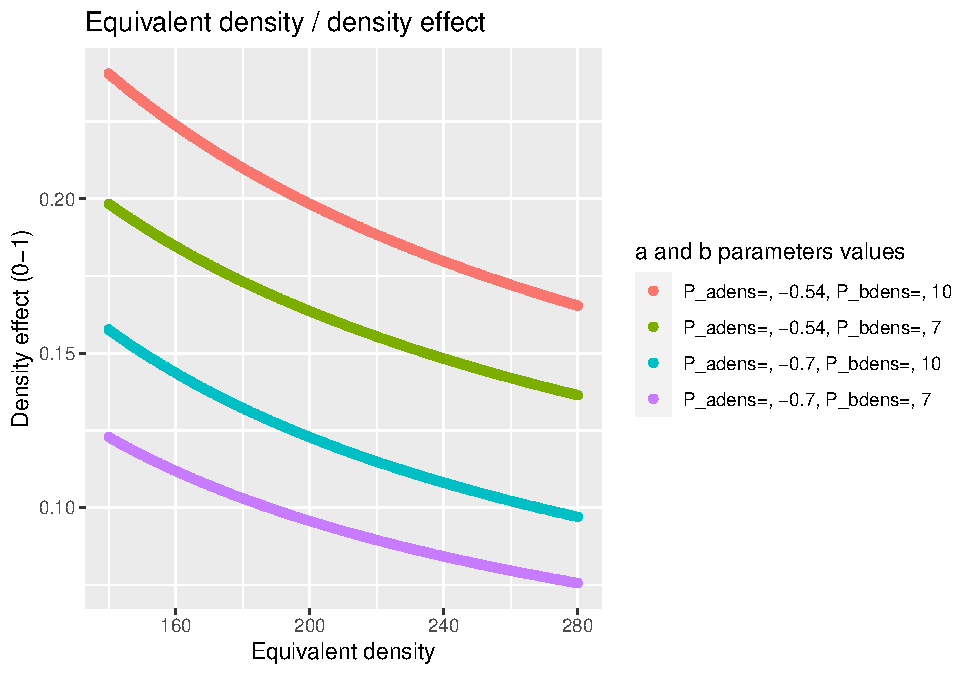
\includegraphics{Postdoc_steps_files/figure-latex/unnamed-chunk-17-1.pdf}

So the higher the density, the higher the negative effect on \texttt{LAI}.

\hypertarget{the-equivalent-density}{%
\section{The equivalent density}\label{the-equivalent-density}}

In sole crops, the density effect is straightforward. However, under the case of mixed crops, the density effect can be higher for the dominated plant compared to its equivalent in sole crops. Indeed, a pea in sole crop would have a given competition with other close plants, but a different one when mixed with wheat, where the same density of wheat can give higher competition effect for light because it is taller.

Then the density effect is computed as an equivalent density instead (\texttt{densiteequiv}), that can differ from the sowing density for the dominated crop to increase the negative effect of \texttt{efdensite} compared to a sole crop.

The previous implementation in STICS was simple. As soon as a plant become dominated, it had an increased equivalent density compared to its actual density (\emph{e.g.} doubled). After some discussion with the STICS intercrop team, this formalism was considered not suitable for two reasons:

\begin{itemize}
\item
  Whenever a plant become shorter its density drastically increases regardless of the height difference. We propose to modify the formalism to consider the height difference explicitly while computing the equivalent density.
\item
  For the moment, the competition induced by the density of the other species (\emph{i.e.} interspecies competition) was re-included in the equivalent density computation using the \texttt{P\_bdensp1} and \texttt{P\_bdensp2} parameters, which come from the sole crop formalism, where it is used to consider intra-species competition effect. The equivalent density was originally set up to consider the decrease in light quality when a plant has another plant above it. Adding another computation of competition based on the density of the other plant could be redundant, because it is already considered during the light interception (see Chapter \ref{Interrow} and \ref{Light}). Consequently, we propose to remove this computation from the equivalent density formalism, and to let the \texttt{P\_bdensp1} and \texttt{P\_bdensp2} parameters being used to compute the \texttt{efdensite} variable only.
\end{itemize}

\hypertarget{proposition-for-new-equivalent-density-formalism}{%
\section{Proposition for new equivalent density formalism}\label{proposition-for-new-equivalent-density-formalism}}

\hypertarget{definition-of-the-different-propositions}{%
\subsection{Definition of the different propositions}\label{definition-of-the-different-propositions}}

The user will now have four options to compute the equivalent density, depending on the value of the \texttt{P\_code\_calc\_equi\_density} parameter:

\begin{itemize}
\item
  (1): Previous computation : \(density_{Equivalent}= density_{p2} + \frac{density_{p1}}{P_{bdensp1}}\cdot P_{bdensp2}\)
\item
  (2): Improved computation to define the equivalent density as a function of the height difference between the plants as follow:
  \(density_{Equivalent} =\begin{cases}\Delta_{height} > hauteur_{threshold} & density_{p2} + \frac{density_{p1}}{P_{bdensp1}}\cdot P_{bdensp2} \\ \Delta_{height} < hauteur_{threshold} & density_{p2}+slope\cdot abs\left|\Delta_{height}\right| \end{cases}\)\\
  with \(diffx= \frac{density_{p1}}{P_{bdensp1}}\cdot P_{bdensp2}\) and \(slope= \frac{diffx}{hauteur_{threshold}}\)
\item
  (3): Improved computation to define the equivalent density as a function of the height difference between the plants, and using different parameters for intraspecific and interspecific competition, with simpler meanings. This formalism would give no increase in equivalent density until a given threshold (\texttt{hauteur\_threshold}), after which a progressive increase in the equivalent density would happen until the maximum allowed. In this computation, the slope would be computed by the model, and the equivalent density would be computed as follows: \(density_{Equivalent} =\begin{cases}\Delta_{height} < hauteur_{threshold} & density_{p2} \\ \Delta_{height} > hauteur_{threshold} & b + \Delta_{height}\cdot slope \\ \Delta_{height} > hauteur_{threshold_2} & Max_{equDens} \end{cases}\)\\
  with \(slope= \frac{Max_{equDens}}{hauteur_{threshold_2}-hauteur_{threshold}}\).
  This formalism would include three parameters:

  \begin{itemize}
  \item
    \texttt{hauteur\_threshold}: the difference in height below which no competition is occuring
  \item
    \texttt{hauteur\_threshold\_2}: the difference in height below which a progressive competition is occuring
  \item
    \texttt{Max\_equDens}: the maximum equivalent density allowed (generally the sole crop density).
  \end{itemize}
\item
  Any other value: the equivalent density is equal to the true plant density
\end{itemize}

\hypertarget{visual-representation-of-the-options}{%
\subsection{Visual representation of the options}\label{visual-representation-of-the-options}}

The two new formalisms are both linking the equivalent density to the difference of height between the two plants, but using different parameters and outputs.

Here is a visual representation of the equivalent density when \texttt{P\_code\_calc\_equi\_density=\ 2} for a wheat-pea intercrop with a plant density of 140 for the wheat as the principal species and 30 for the pea as the associated species:

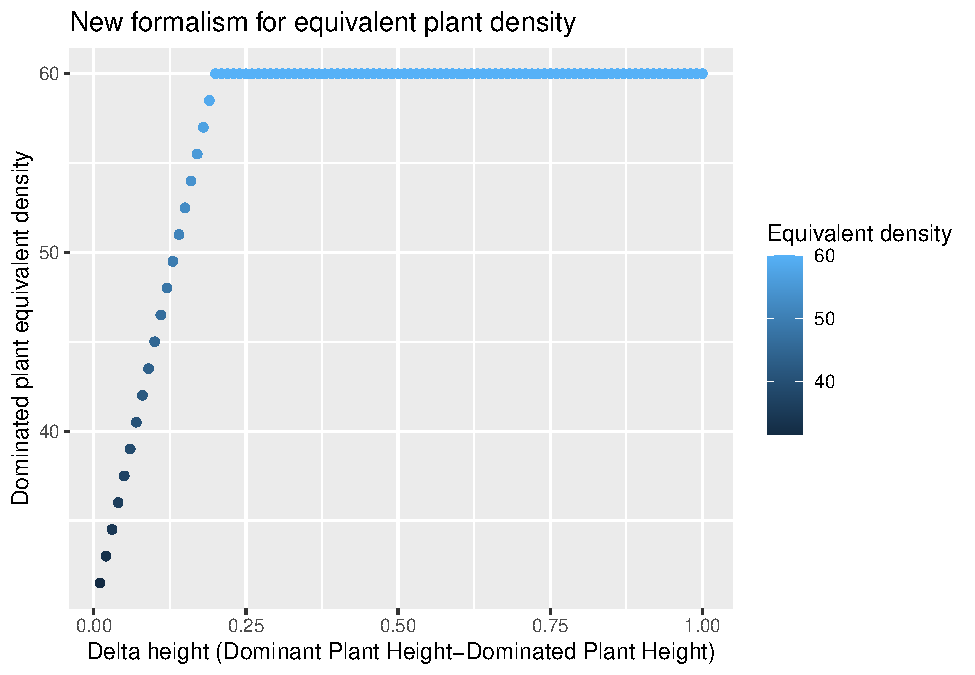
\includegraphics{Postdoc_steps_files/figure-latex/P_code_calc_equi_density_2-1.pdf}

This option has several implications in the model, notably that the dominated plant is less impacted by the competition with the dominant plant when both have approximately the same height.

Here is a visual representation of the same output when \texttt{P\_code\_calc\_equi\_density=\ 3}:

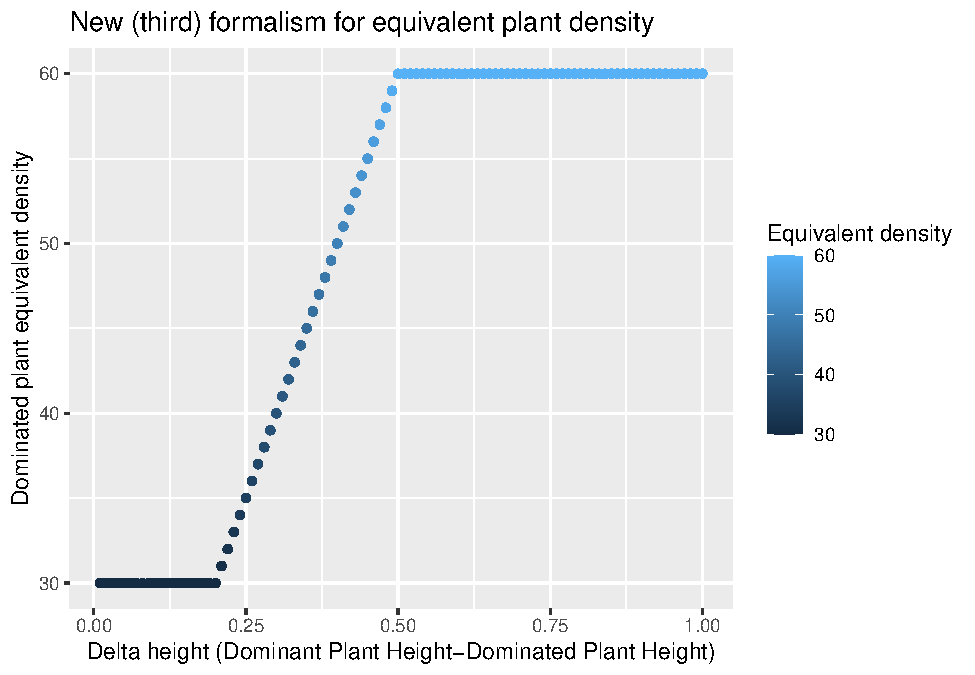
\includegraphics{Postdoc_steps_files/figure-latex/P_code_calc_equi_density_3-1.pdf}

This formalism considers no interspecific competition for the quality of light while the difference in height is low, and then an increased competition until a maximum is reached.

\hypertarget{comparison-between-options}{%
\subsection{Comparison between options}\label{comparison-between-options}}

A comparison of the different formalisms was made using the \href{https://github.com/VEZY/sticRs}{sticRs} package, from which a summary plot was extracted, and the results are shown in Figure \ref{fig:trgcomparison2}.

\begin{figure}
\centering
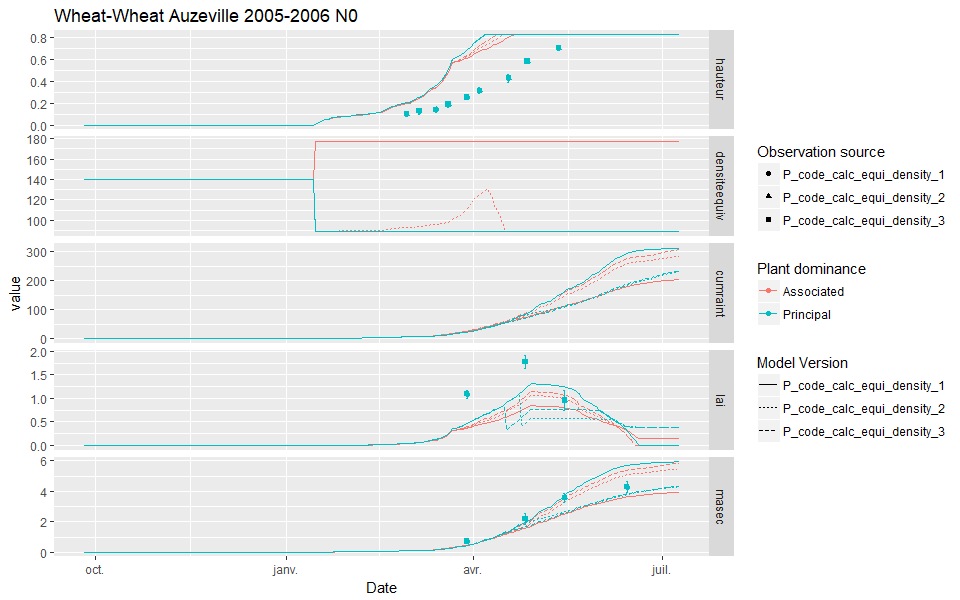
\includegraphics{img/Equi_dens_3.png}
\caption{\label{fig:trgcomparison2}Comparing options for the equivalent density computation}
\end{figure}

It is not very clear from the figure, but the second and third options (\emph{i.e.} \texttt{P\_code\_calc\_equi\_density=\ 2} and \texttt{P\_code\_calc\_equi\_density=\ 3}) for the equivalent density computation are both less severe than the previous one (\texttt{P\_code\_calc\_equi\_density=\ 1}) for the dominated plant. The second one has effect on the equivalent effect for limited time only (dashed red curve), while the third one show no increase in equivalent density all along the crop life because the height difference remains below the first threshold. Consequently, the dominated plant intercepts more light (see \texttt{cumraint} and \texttt{fapar}) and has a higher \texttt{LAI} using the third option.

\hypertarget{Interrow}{%
\chapter{Interrow spacing}\label{Interrow}}

\hypertarget{introduction-3}{%
\section{Introduction}\label{introduction-3}}

The inter-row is the distance between two rows of the same plant species. Figure \ref{fig:SameInterrow} shows a simple design with a field with two plant species sowed with the same inter-row.

\begin{figure}
\centering
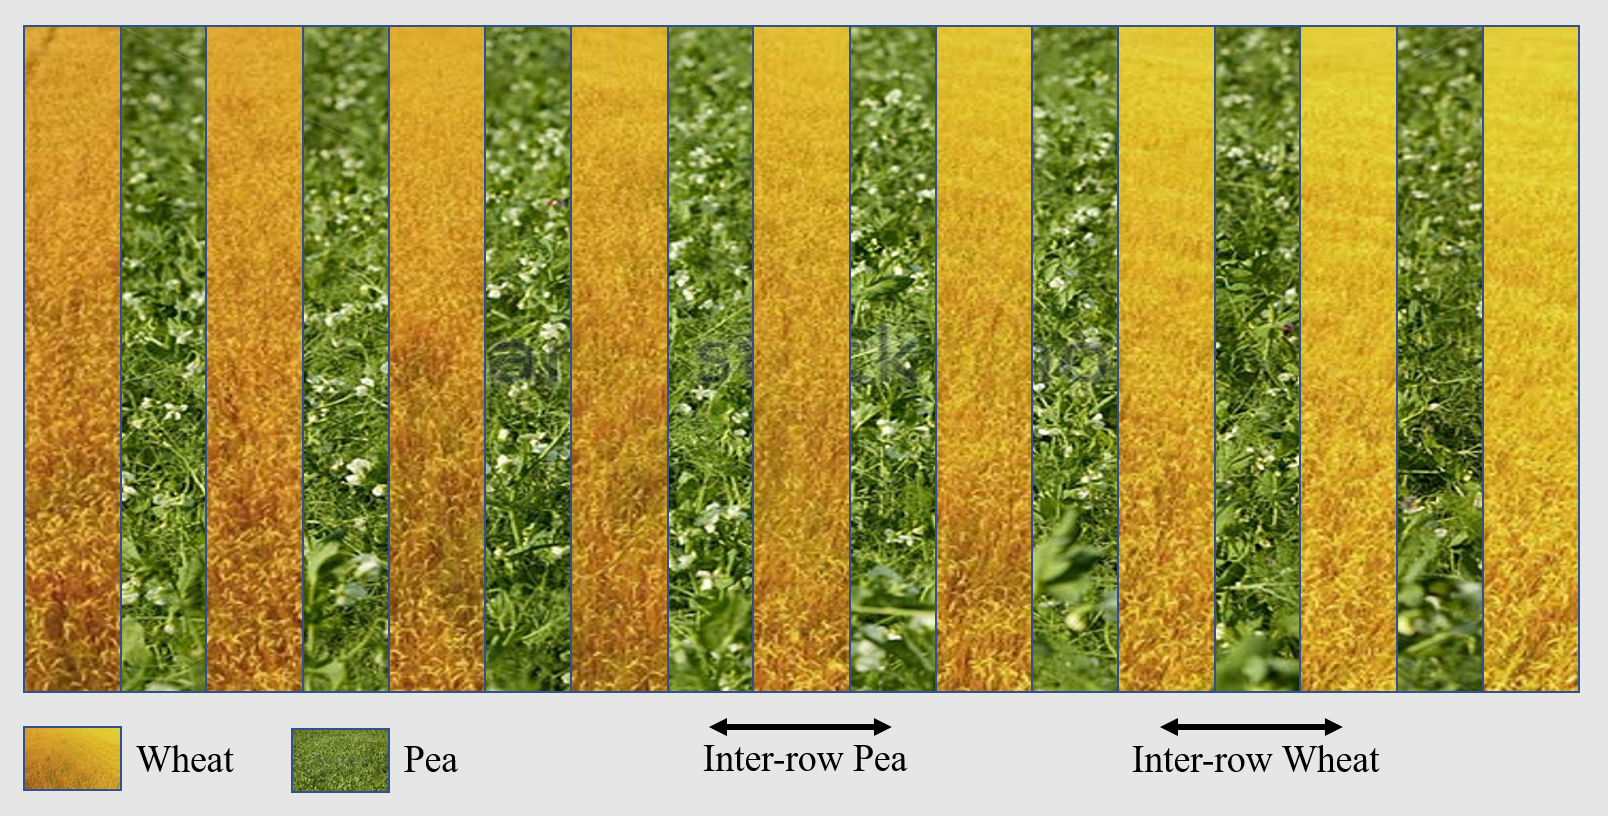
\includegraphics{img/Same-Interrow.png}
\caption{\label{fig:SameInterrow}Pea-Wheat intercrop using the same inter-row spacing for the two crops}
\end{figure}

So far, so good. Now what happens if we set a different inter-row spacing for the two species ?

\hypertarget{inter-row-spacing-for-mixed-crops-in-the-model}{%
\section{Inter-row spacing for mixed crops in the model}\label{inter-row-spacing-for-mixed-crops-in-the-model}}

Whereas the model as a notion of the position of the plants along the interrow considering the same plant species (\emph{i.e.} Principal or Associated), it does not explicitly position the different plant species between each other. Indeed, the light interception of the dominant plant is first computed using its geometry and a plane at the height of the dominated plant. Then, the light interception of the dominated plant is computed using the average light incident on the previous plane (separated between shaded and sunlit component), the plant geometry, and a second plane right above the soil. So when computing its light interception, the dominated plant do not consider at all the dominant plant interrow spacing, but only the light it transmits. Of course the dominant plant interrow spacing does impact the light that is transmitted to the dominatd plant, but it is not an explicit description of the interrow spacing.

Figure \ref{fig:interrow} shows a depiction of how the model describe the interrow for intercrops.

\begin{figure}
\centering
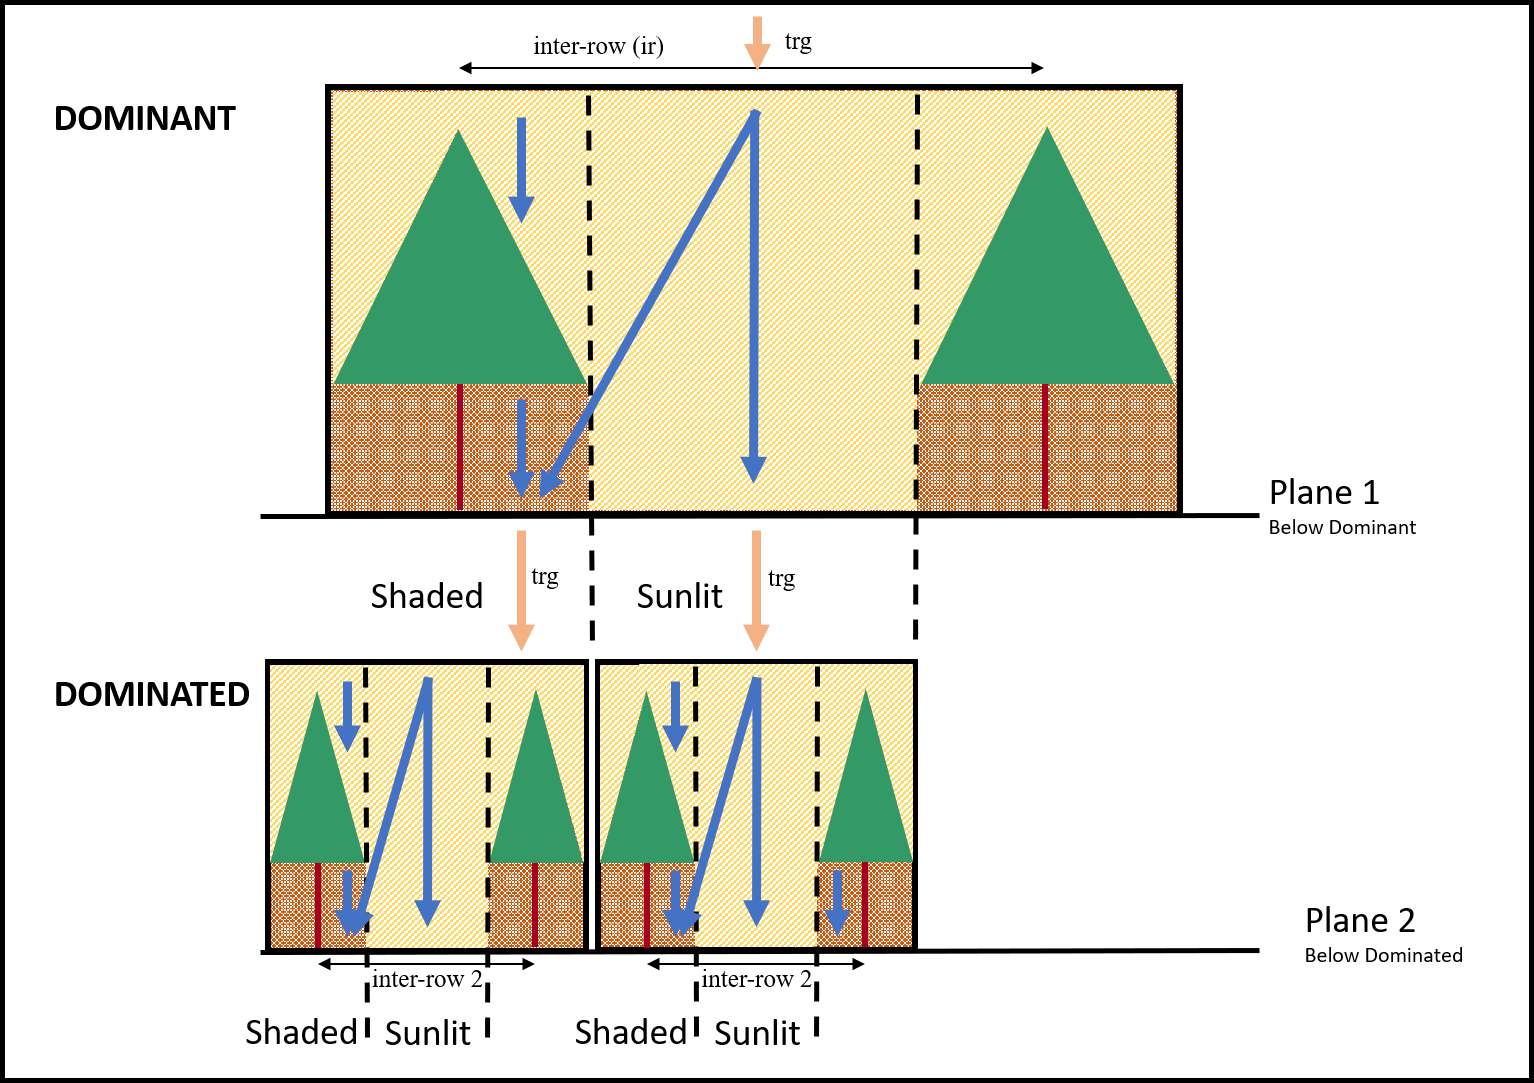
\includegraphics{img/Interrow.png}
\caption{\label{fig:interrow}Interrow effect on light interception for intercrops in the STICS model}
\end{figure}

The model does effectively compute half the interrow light interception only, because it is assumed that the other half have the same light regime at daily time-scale.
First the interrow of the dominant plant is used to position the left and right dominant plants. The model then computes the golbal radiation (\texttt{trg}) that is transmitted to the Plane 1, which is then used to compute the light intercepted by the dominant plant. The light transmitted to the Plane 1 is divided into two light regimes: a shaded component (surface right under the dominant plant canopy) and a sunlit component (the opposite).

Second, the light incident on the Plane 1 is used as the \texttt{trg} for the dominated plant, and the same computation than for the dominant plant is performed for the shaded and sunlit components of the dominated plant, and then integrated at species-scale using both light interception and relative surface.

To conclude on this point, we see that the interrow spacing can only impact the light interception as a density effect (more plants per m2, closer intra-species canopy), but not as a pure geometrical effect.

For more details on how the \texttt{trg} is computed, see Chapter \ref{trg}, and for more details on light interception, see Chapter \ref{Light}.

\hypertarget{design}{%
\chapter{Design}\label{design}}

\hypertarget{introduction-4}{%
\section{Introduction}\label{introduction-4}}

It is difficult to understand well which cropping design (i.e.~species arrangement) can be simulated using the STICS model formalisms. Based on the previous information from Chapter \ref{Light}, \ref{trg}, and \ref{Interrow}, we present some use-cases were the model can be applied according to its formalisms, and were it cannot.
The list of designs proposed here is not exhaustive, and the user should always think about the relevance of using STICS to model a particular design.

\hypertarget{designs-that-can-be-simulated}{%
\section{Designs that can be simulated}\label{designs-that-can-be-simulated}}

Figure \ref{fig:DesignOK} shows the depiction of some of the cropping designs that possibly can be simulated by the STICS model. The list is not exhaustive, but gives an overall look on the possibilities:

\begin{figure}
\centering
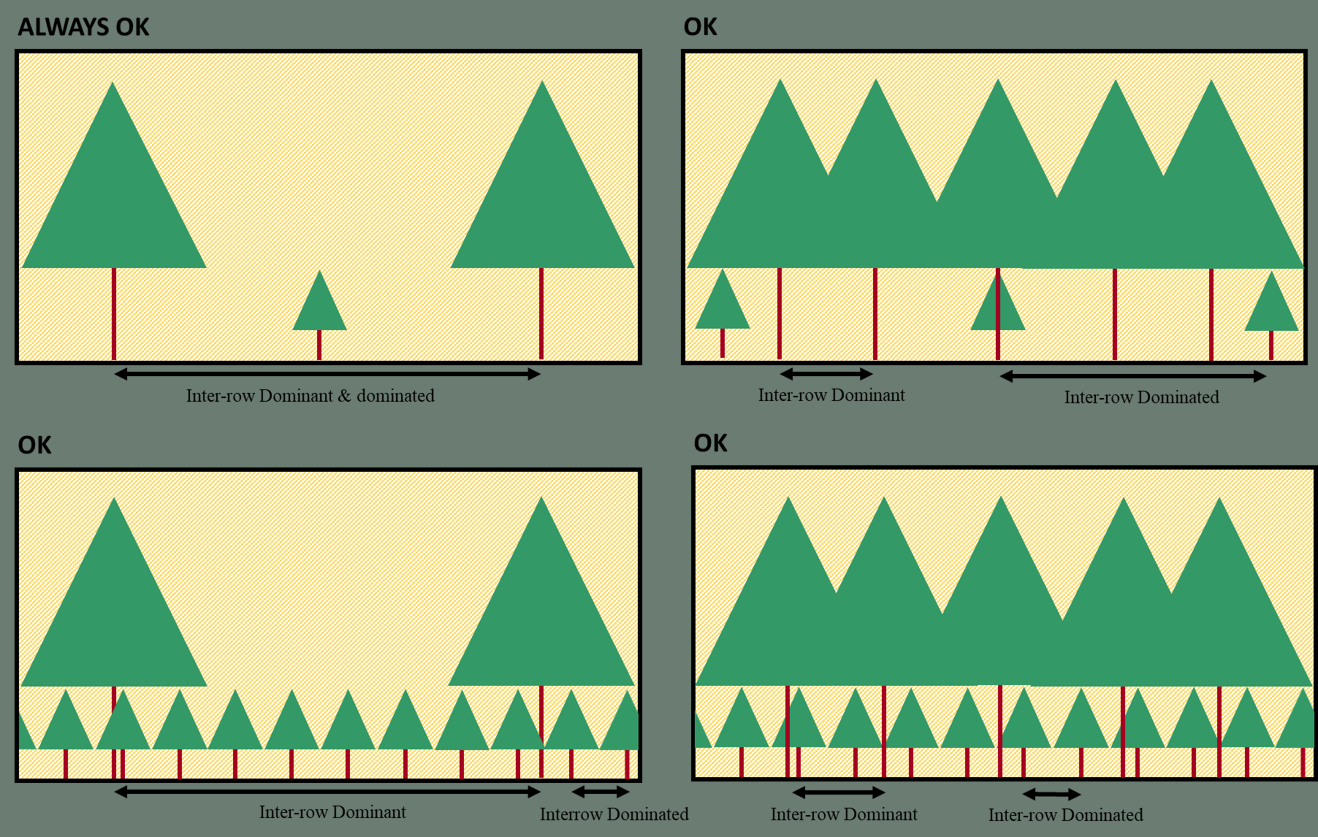
\includegraphics{img/Design_OK.png}
\caption{\label{fig:DesignOK}Depiction of the potentially adapted intercrop designs for simulation using the STICS model.}
\end{figure}

The list will be extended soon, and the different assumptions and domain of vailidity for each will be detailed too.

\hypertarget{designs-that-cannot-be-simulated}{%
\section{Designs that cannot be simulated}\label{designs-that-cannot-be-simulated}}

Figure \ref{fig:DesignKO} shows a design that cannot be simulated by the STICS intercrop model as is:

\begin{figure}
\centering
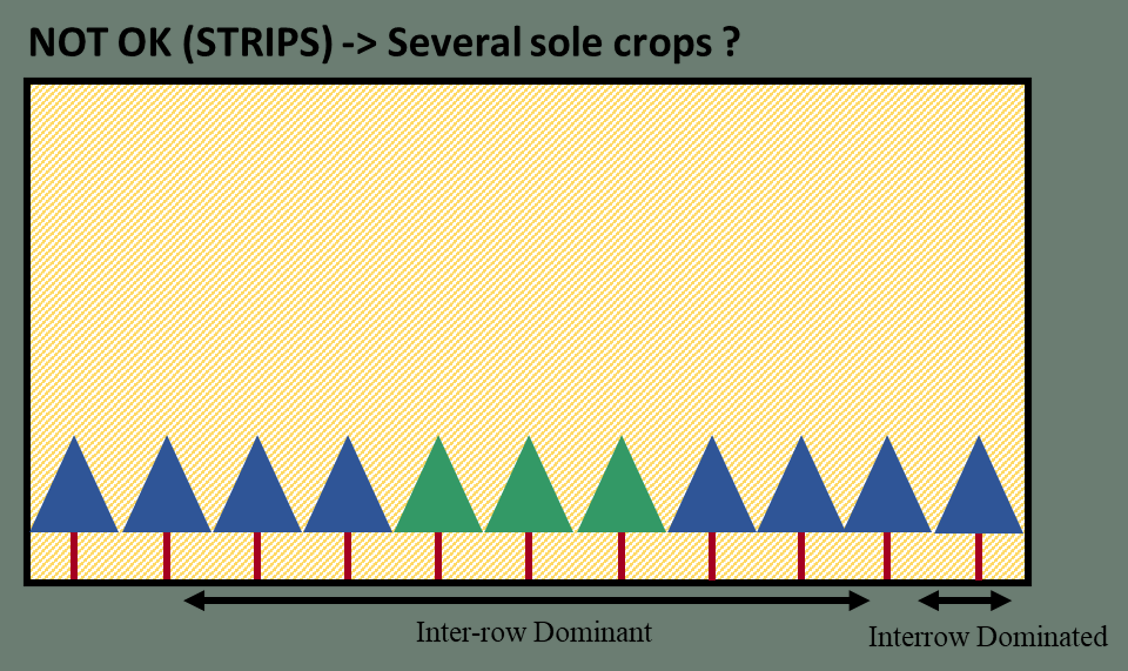
\includegraphics{img/Design_KO.png}
\caption{\label{fig:DesignKO}Depiction of the intercrop designs not adapted for simulation using the STICS model as is.}
\end{figure}

Indeed, strips implies that interspecies light competition is only present on the border of each strip, making the Dominant/Dominated paradigm unreallistic for this design. The model could simulate large strips as two separated crops though.

\hypertarget{LAIissue}{%
\chapter{Issue on LAI not decreasing}\label{LAIissue}}

\hypertarget{introduction-5}{%
\section{Introduction}\label{introduction-5}}

The \texttt{LAI} is not decreasing on the end of the crop cycle for the dominant plant (Figure \ref{fig:LAIhigh}).

\begin{figure}
\centering
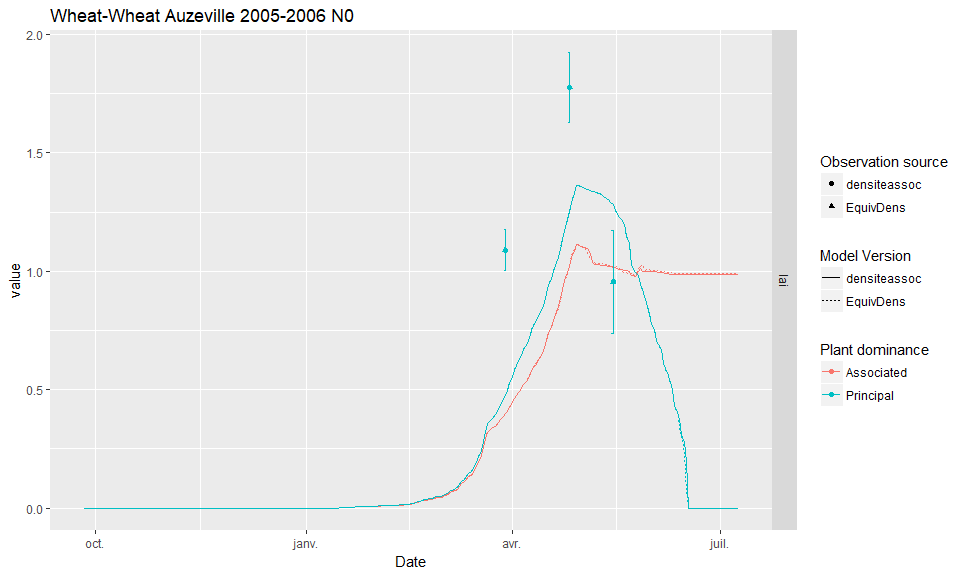
\includegraphics{img/LAI_high.png}
\caption{\label{fig:LAIhigh}Leaf Area Index in a self-intercrop of Wheat-Wheat}
\end{figure}

This issue can have different origins. The main hypothesis are:

\begin{itemize}
\tightlist
\item
  The leaf surface may be too high compared to their mass, coming from an abnormally high \texttt{sla}\\
\item
  A too low senescence, coming itself from a too long leaf lifespan, which could arise from a too low nitrogen mobilization (increase the lifespan), and/or a too low water stress (water stress can decrease the life span).
\end{itemize}

\hypertarget{investigating-the-sla-hypothesis}{%
\section{Investigating the sla hypothesis}\label{investigating-the-sla-hypothesis}}

Figure \ref{fig:LAISLA} shows that both plants (\emph{i.e.} Principal and Associated) have exactly the same \texttt{SLA} during the growing cycle. This discard the possibility of a problem coming from a wrong \texttt{SLA} because it would be much higher for the plant with the constant \texttt{LAI} at the end of the cycle.

\begin{figure}
\centering
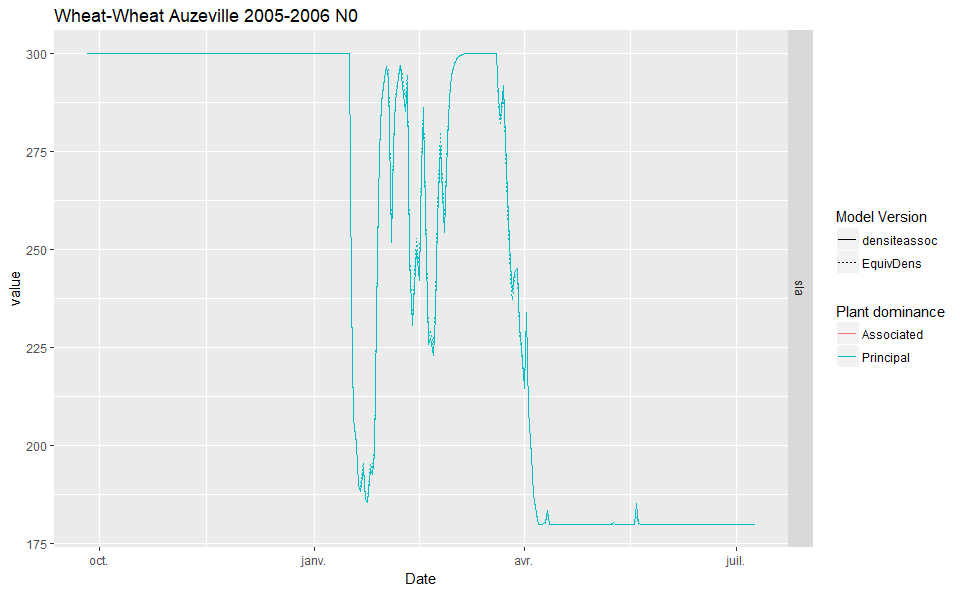
\includegraphics{img/LAI_hyp_SLA.png}
\caption{\label{fig:LAISLA}Specific Leaf Area in a self-intercrop of Wheat-Wheat}
\end{figure}

\hypertarget{leaf-senescence}{%
\section{Leaf senescence}\label{leaf-senescence}}

Leaf senescence is actually much lower for the plant that has a non-decreasing \texttt{LAI} (Figure \ref{fig:Leafsen})

\begin{figure}
\centering
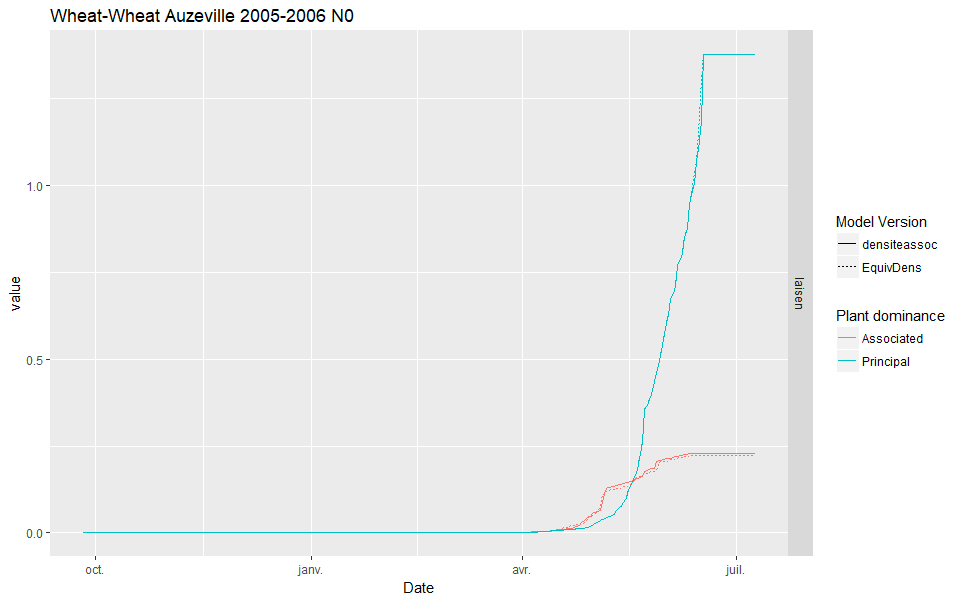
\includegraphics{img/Senescence.png}
\caption{\label{fig:Leafsen}Leaf Senescence in a self-intercrop of Wheat-Wheat}
\end{figure}

The next step is to find out why leaf senescence is too low for this plant.

\hypertarget{leaf-lifespan}{%
\subsection{Leaf lifespan}\label{leaf-lifespan}}

The Figure \ref{fig:Durvie} shows that the leaf lifespan is not much different between both plants either, rejecting our hypothesis of a too long lifespan.

\begin{figure}
\centering
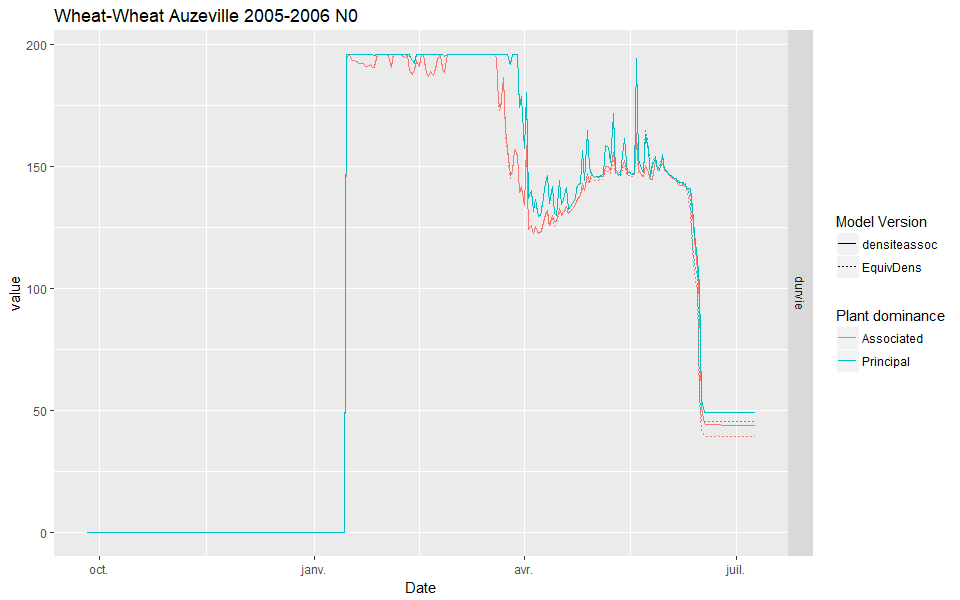
\includegraphics{img/Durvie.png}
\caption{\label{fig:Durvie}Leaf Lifespan in a self-intercrop of Wheat-Wheat}
\end{figure}

However, printing the lifespan for each light environment (\emph{i.e.} shaded, sunlit) showed that the lifespan of the shaded part of the dominated plant was equal to 0 most of the time, making \texttt{nsencours} jump from \texttt{nlev} to the first day when senescence is computed (here at day 208) at once (Figure \ref{fig:nsencour}).

\begin{figure}
\centering
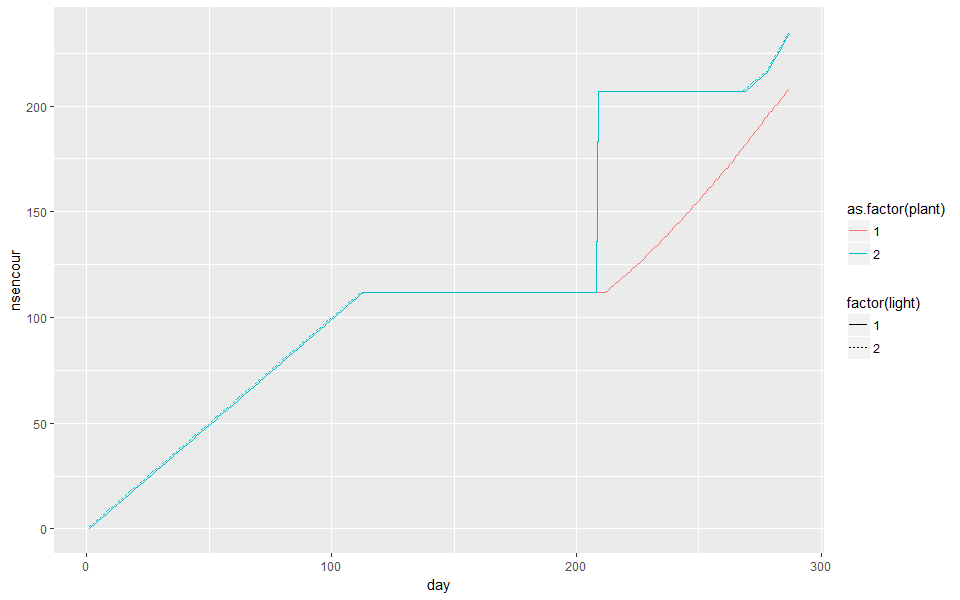
\includegraphics{img/LAIhigh_nsencour.png}
\caption{\label{fig:nsencour}Leaf (lai) appearence day (\texttt{nsencour}) compared to the day (\texttt{day}) they become senescent (self-intercrop of Wheat-Wheat)}
\end{figure}

The leaf lifespan (\texttt{durvie(i)}) was computed as:

The bug came from the computation of \texttt{durvie(i)} that was initialized to 0, and always equal to 0 afterward until the \texttt{fin} was reached.\\
A correction is proposed to fix the bug, which make the same computation except on the first day on which the senescence is computed (\texttt{nsencour==nlev}):

The new computation fix the bug, making \texttt{nsencour} more progressive as for the dominated plant (Figure \ref{fig:nsencourfix}).

\begin{figure}
\centering
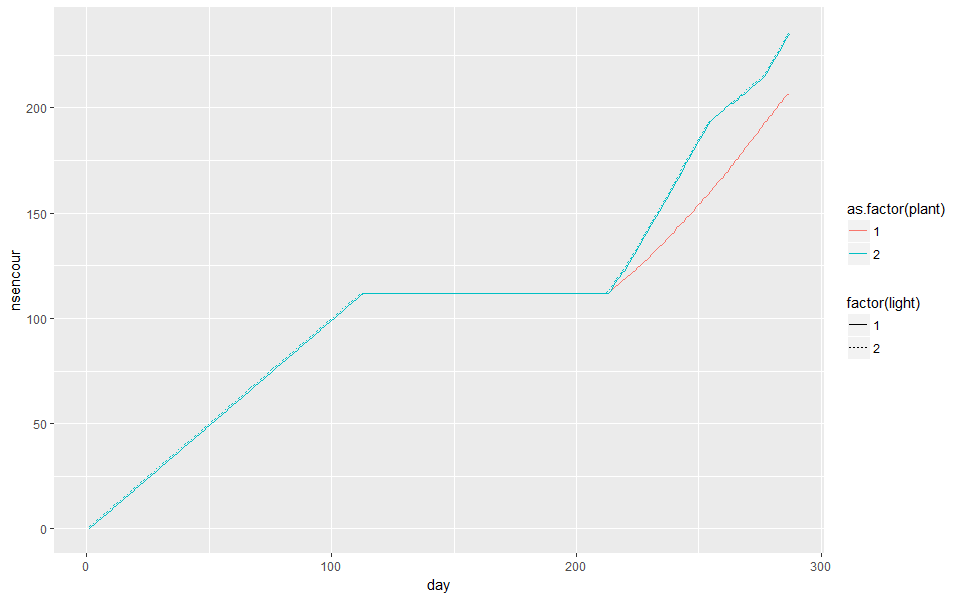
\includegraphics{img/LAIhigh_nsencourfix.png}
\caption{\label{fig:nsencourfix}Leaf (lai) appearence day (\texttt{nsencour}) compared to the day (\texttt{day}) they become senescent using the new computation of durvie (self-intercrop of Wheat-Wheat)}
\end{figure}

\hypertarget{stress-indices}{%
\subsection{Stress indices}\label{stress-indices}}

The senescence is computed using leaf life span, but also two different stress indices: \texttt{senfac} for the water stress and \texttt{innsenes} for the nitrogen stress.
Figure \ref{fig:senstress} shows that the plant with non-decreasing \texttt{LAI} has a higher stress compared with the other plant, rejecting again the hypothesis of a too low stress indices.

\begin{figure}
\centering
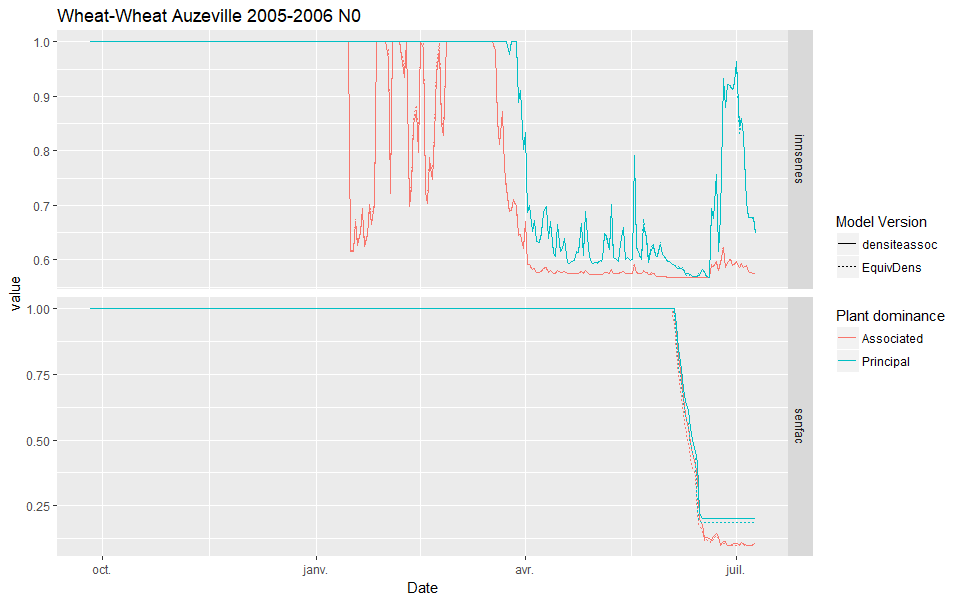
\includegraphics{img/sen_stress.png}
\caption{\label{fig:senstress}Stress index to compute leaf lifespan in a self-intercrop of Wheat-Wheat}
\end{figure}

\hypertarget{over-fertilization}{%
\subsection{Over-fertilization}\label{over-fertilization}}

The problem could arise from a nitrogen over-fertilization (\texttt{inn}) that could increase lifespan, but the Figure \ref{fig:overfert} shows the contrary, with a lower \texttt{inn} for the plant with non-decreasing \texttt{LAI}.

\begin{figure}
\centering
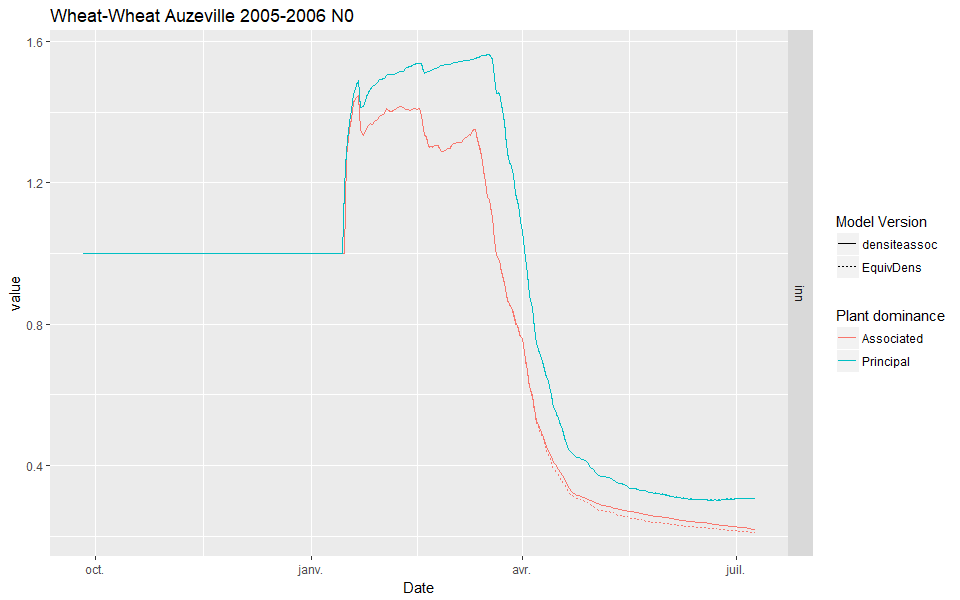
\includegraphics{img/overfert.png}
\caption{\label{fig:overfert}Nitrogen over-fertilization in a self-intercrop of Wheat-Wheat}
\end{figure}

\hypertarget{de-activating-water-and-nitrogen-stresses}{%
\subsection{De-activating water and nitrogen stresses}\label{de-activating-water-and-nitrogen-stresses}}

To check if the senescence is still related to water and nitrogen stresses, Figure \ref{fig:nostress} shows a simulation where both effects are removed (\texttt{P\_codeh2oact=\ 2} and \texttt{P\_codeinnact=\ 2}).

\begin{figure}
\centering
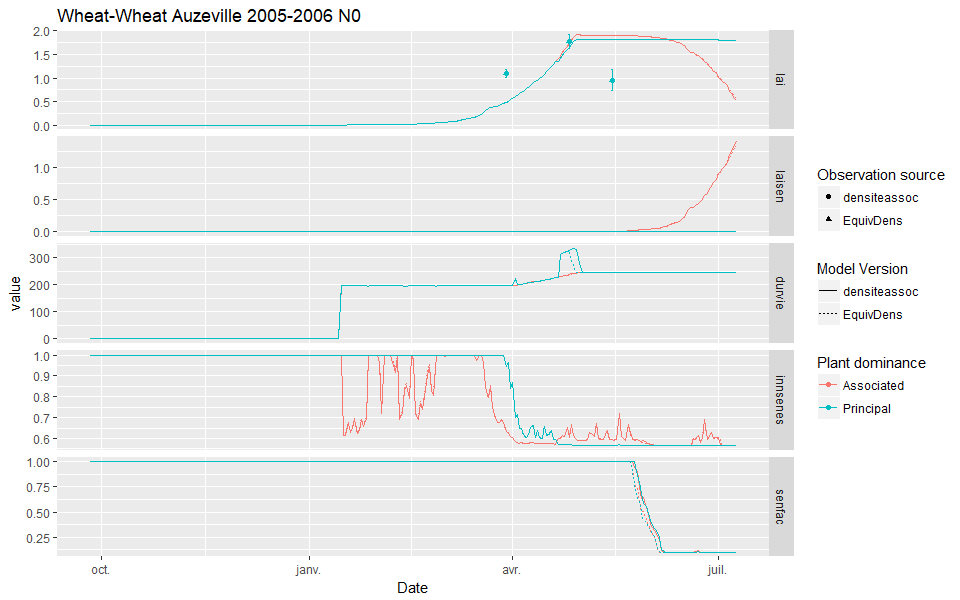
\includegraphics{img/nostress.png}
\caption{\label{fig:nostress}Simulation of a Wheat-Wheat self-intercrop with no nitrogen and water stresses}
\end{figure}

Removing the stress do not change the fact that one plant has a constant \texttt{LAI} at the end of the crop cycle. This proves that the problem does not arise from a limitation in water or nitrogen.

\hypertarget{the-solution-to-the-first-issue}{%
\section{The solution to the first issue}\label{the-solution-to-the-first-issue}}

Three main variables were badly used to compute the senescence: \texttt{dltams}, \texttt{deltai} and \texttt{pfeuilverte}. These variables correspond to the daily increment in dry mass, daily increment in lai, and the green leaves proportion. The model used the values from previous computations kept in memory to compute the different components of the senescence for each light environment of the plant (\emph{i.e.} sunlit or shaded) separately.

Unfortunately, the dominance of the plant can change over time, so a dominant plant with no shaded component can have one afterwards. If a dominant plant becomes dominated, the model was trying to use \texttt{dltams}, \texttt{deltai} and \texttt{pfeuilverte} of the shaded part of the plant that all were equal to 0 (as their initialization) because they were not computed before, making no senescence at all for the shaded part of the plant.

We propose to replace the use of a separated shaded and sunlit \texttt{dltams}, \texttt{deltai} and \texttt{pfeuilverte} by their total at plant level, weighted by their relative surface under shaded and sunlit environment. For example, the \texttt{deltai} input to the \texttt{senescen} function would be \texttt{p(i)\%deltai(0,1:sc\%nbjmax)*p(i)\%surf(ens)} instead of \texttt{p(i)\%deltai(ens,1:sc\%nbjmax))}, with \texttt{p(i)\%deltai(0,n)\ =\ p(i)\%deltai(sc\%AS,n)*\ p(i)\%surf(sc\%AS)\ +\ p(i)\%deltai(sc\%AO,n)*\ p(i)\%surf(sc\%AO)}. This new computation has the advantage of considering all the lai that was incremented before, with a drawback being not to consider the previous relative surface of the plant.

Figure \ref{fig:Newsen} shows the resulting outputs, which are more realistic.

\begin{figure}
\centering
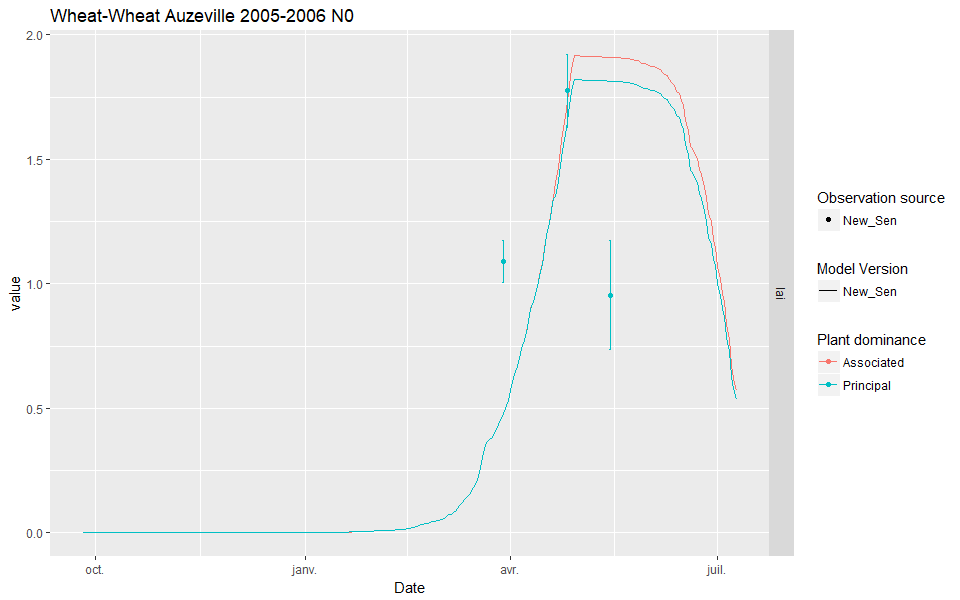
\includegraphics{img/Newsen.png}
\caption{\label{fig:Newsen}Simulation of a Wheat-Wheat self-intercrop leaf area index using the modified STICS version}
\end{figure}

\hypertarget{fixing-a-second-issue}{%
\section{Fixing a second issue}\label{fixing-a-second-issue}}

After adressing the first issue, I added the new formalism to compute the equivalent density (see Chapter \ref{plantdensity}). While studying the effect of this new formalism, I stumbled upon the same apparent issue : the \texttt{lai} was not decreasing at the end of the crop cycle. This issue came from the fact that the sharing of the \texttt{deltai} for the dominated plant between the shaded and sunlit components was too simple (see previous paragraph). Indeed, the \texttt{deltai} was weighted according to their respective surface of the current day (\texttt{n}), but the senescence can happen on different days (and it is) because both light components do not experience the same temperature conditions, so the surface effectively used to wheight \texttt{deltai} can be different from one day to another, making either the total dominated plant \texttt{deltai} too high or too low, as seen in Figure \ref{fig:ReSen}, which shows an \texttt{lai} that do not go down to 0 at the end of the crop cycle.

\begin{figure}
\centering
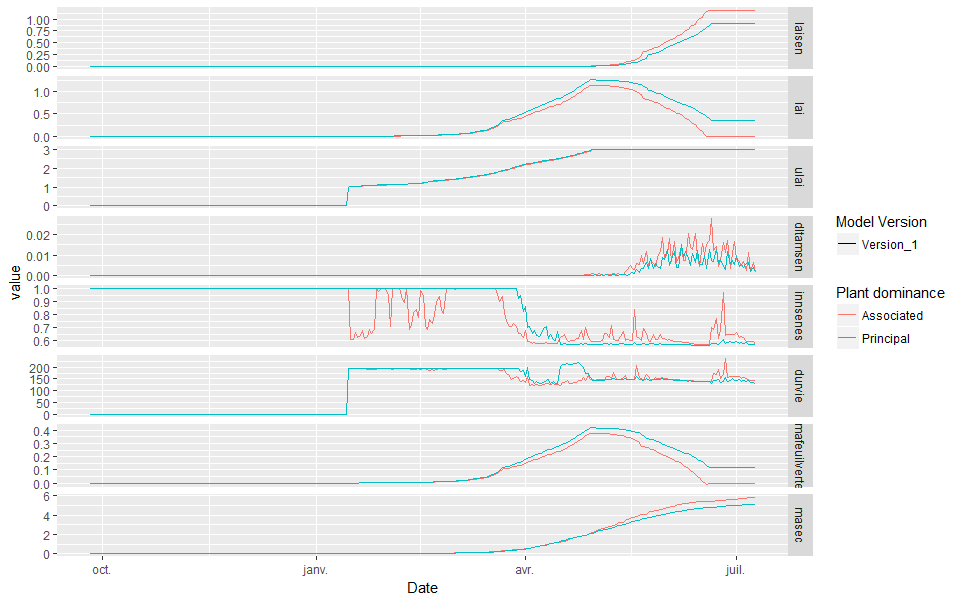
\includegraphics{img/ReSen.png}
\caption{\label{fig:ReSen}Simulation of a Wheat-Wheat self-intercrop using STICS showing an issue in the simulation of the lai at the end of the crop cycle}
\end{figure}

The issue was partially fixed by adding a temporary variable (\texttt{deltai\_sencour}) to keep trace of how much and when the senescent \texttt{lai} was created, to remove it from the overall pool (new variable, \texttt{deltai\_tmp}) used by the shaded component afterwards. The simulations outputs using the modified STICS are visible in Figure \ref{fig:ReSenFixed}.

\begin{figure}
\centering
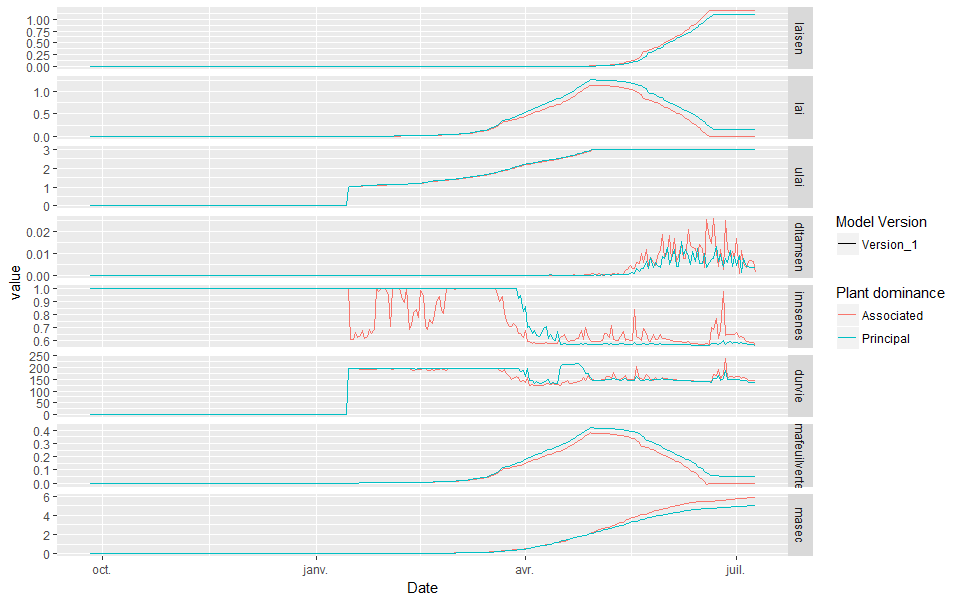
\includegraphics{img/ReSenFixed.png}
\caption{\label{fig:ReSenFixed}Partially fixed issue in the simulation of the lai at the end of the crop cycle}
\end{figure}

This same issue was also found happening for the senescent mass, and the code was modified accordingly to correct it. However, the problem is not entirely solved, because the \texttt{lai} and \texttt{mafeuilleverte} are not going down to 0 at the end of the crop cycle yet.\\
This came from the way the model compute the cumulative sunlit and shaded \texttt{deltai}, \texttt{dltaisen}, \texttt{dltams} and \texttt{pfeuilverte} at the plant level that is not compatible with their new computation anymore, because theiy already are weighted for plant level.
For example, we computed \texttt{dltaisen}as :

So now it is simply computed as:

Figure \ref{fig:ReSenFixed2} shows the results given by the modified STICS, which finally gives a \texttt{lai} and a \texttt{mafeuilleverte} equal to 0 at the end of the cycle.

\begin{figure}
\centering
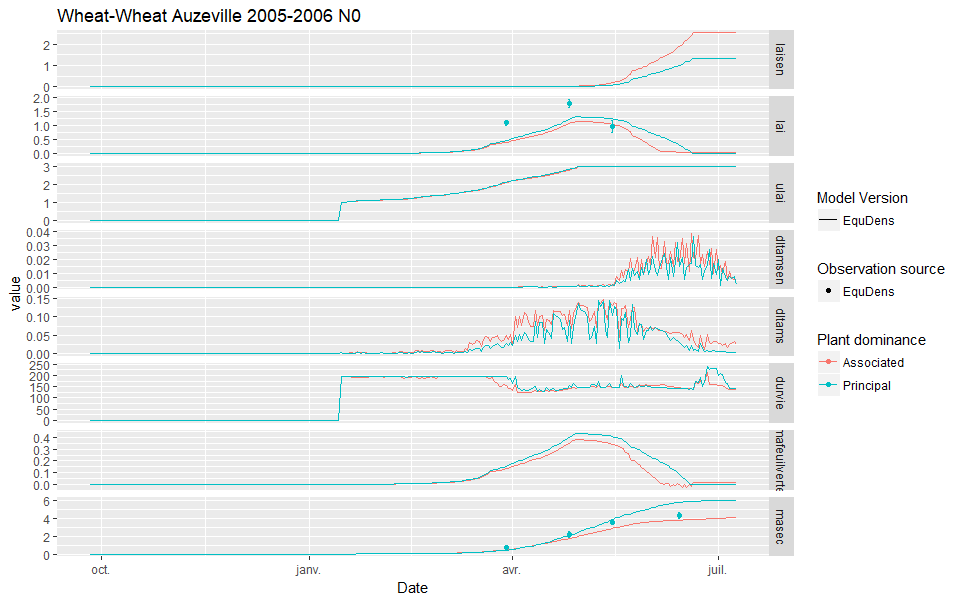
\includegraphics{img/ReSenFixed2.png}
\caption{\label{fig:ReSenFixed2}Fixed issue in the simulation of the masec and lai at the end of the crop cycle}
\end{figure}

\hypertarget{FAPARissue}{%
\chapter{Issue on FaPAR greater than one}\label{FAPARissue}}

\hypertarget{introduction-6}{%
\section{Introduction}\label{introduction-6}}

The fraction of absorbed \texttt{PAR} (\texttt{fapar}) should have values between 0 (no absorption) and 1 (full absorption). The STICS model computed values greater than 1 sometimes (Figure \ref{fig:FAPARhigh}), which is problematic.

\begin{figure}
\centering
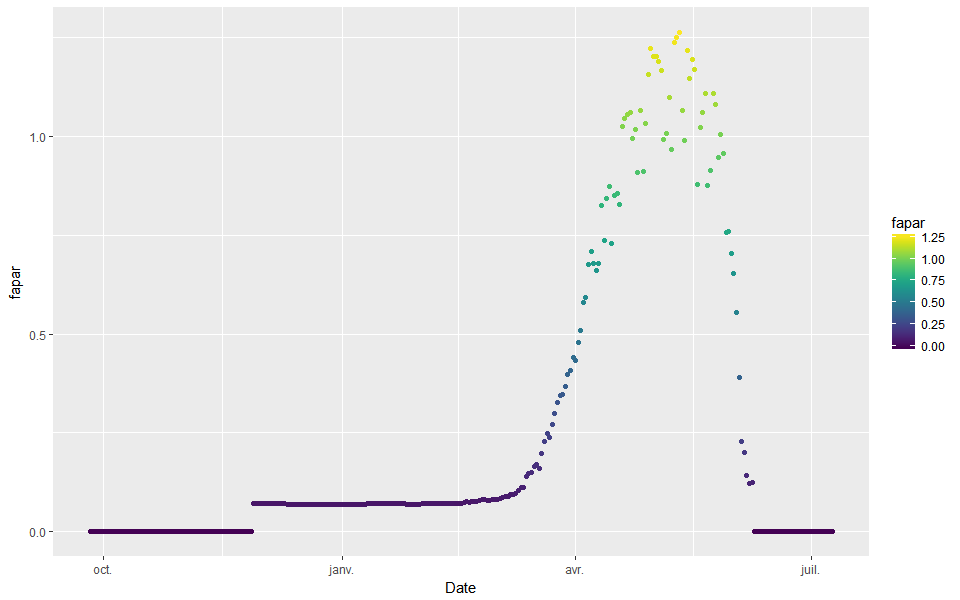
\includegraphics{img/FAPARhigh.png}
\caption{\label{fig:FAPARhigh}Leaf Area Index in a self-intercrop of Wheat-Wheat}
\end{figure}

\hypertarget{the-solution-to-the-problem}{%
\section{The solution to the problem}\label{the-solution-to-the-problem}}

The \texttt{fapar} is computed in the \texttt{raytrans} subroutine, which only uses the \texttt{PAR} transmitted by the dominant plant to a plane above the dominated plant components. This \texttt{PAR} has lower values compared to the atmospheric \texttt{PAR} (\emph{i.e.} from the sky), leading to greater \texttt{fapar}.
We propose to recompute the \texttt{fapar} after the \texttt{biomaer} subroutine to use the atmospheric \texttt{PAR} instead, which is what the user would expect.

The new fapar is now computed as \texttt{p(i)\%fapar(ens)=\ p(i)\%raint(ens)\ /\ (trg\_bak\ *\ pg\%P\_parsurrg)}, and gives better results (Figure \ref{fig:FAPARcorrected}).

\begin{figure}
\centering
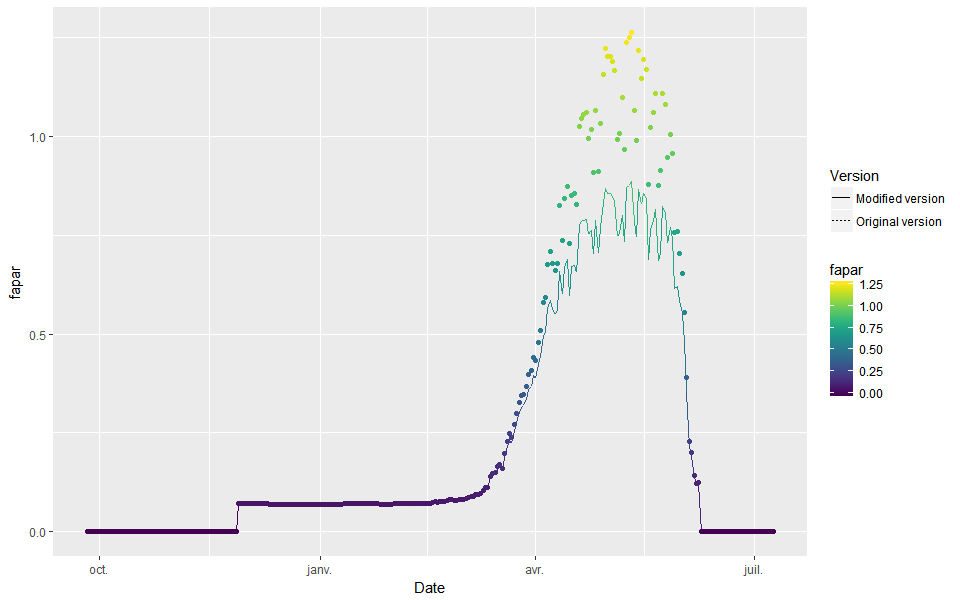
\includegraphics{img/FAPARcorrected.png}
\caption{\label{fig:FAPARcorrected}Leaf Area Index in a self-intercrop of Wheat-Wheat}
\end{figure}

\hypertarget{height}{%
\chapter{Computing plant height}\label{height}}

\hypertarget{introduction-7}{%
\section{Introduction}\label{introduction-7}}

Plant \texttt{height} is not very well simulated for the moment. It is computated using the plant width, which depends itself on the plant \texttt{lai} (\texttt{lai}+\texttt{eai}+\texttt{laisen}). Please see Chapter \ref{Light} for more details. Figure \ref{fig:height1} shows the simulated \texttt{height} of wheat in Auzeville, and the variables from which it is computed.

\begin{figure}
\centering
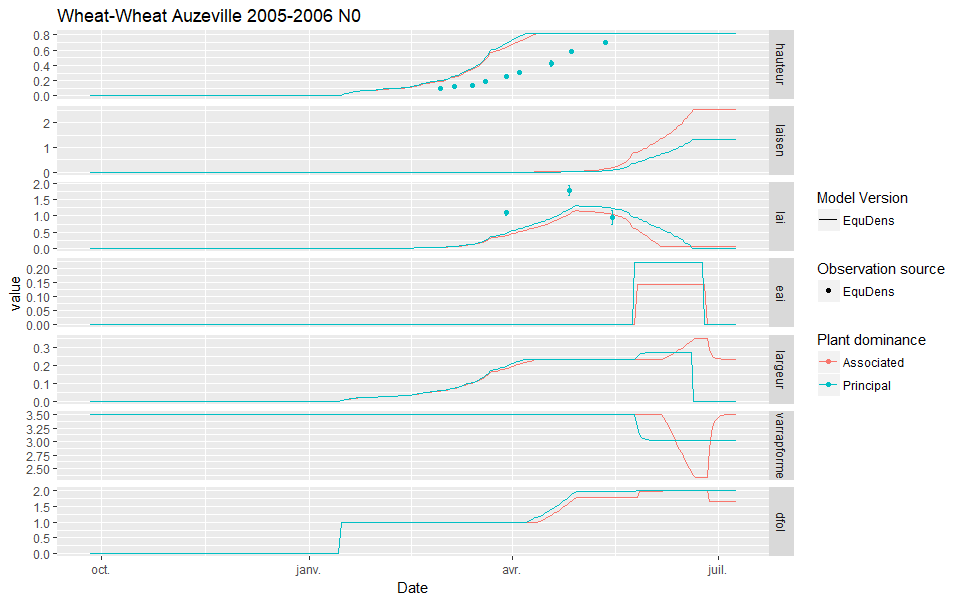
\includegraphics{img/height1.png}
\caption{\label{fig:height1}Simulated height compared to the observed values, and variables from which it is computed from, in a self-intercrop of Wheat-Wheat}
\end{figure}

The plant \texttt{height} is important in the case of intercrops because it has high impact on the light interception of both species.
Indeed, a sensitivity analysis was performed using the \href{https://github.com/VEZY/sticRs}{sticRs} package on the parameter that links the \texttt{lai} to the \texttt{height}: \texttt{P\_rapforme}. The results are shown below (see \texttt{html} version of this book for interactivity):

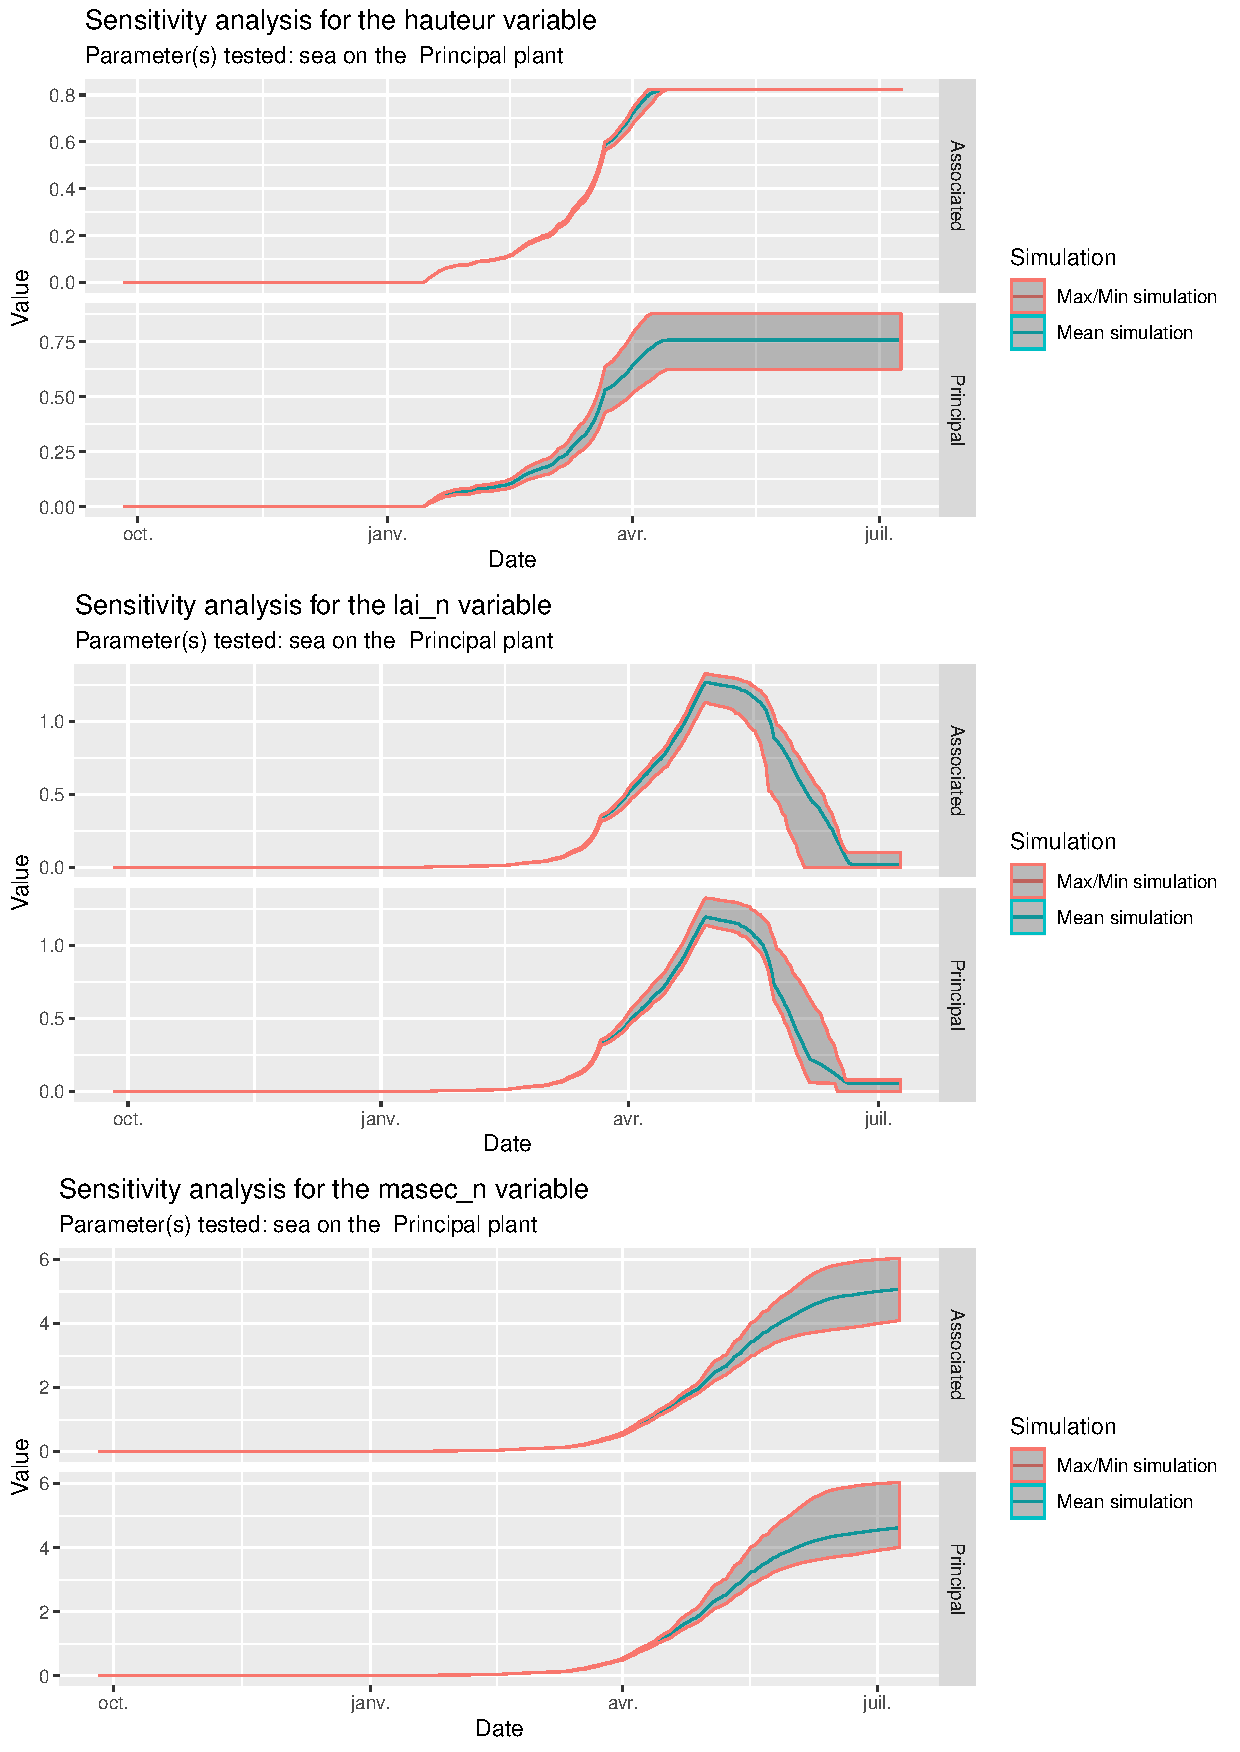
\includegraphics{Postdoc_steps_files/figure-latex/unnamed-chunk-24-1.pdf}

As we can see on the above plots, as the plant \texttt{height} is affected, its \texttt{lai} is also impacted afterwards.
We can also see that no values of \texttt{P\_rapforme} gave satisfactory plant \texttt{height}, so maybe the link between the plant \texttt{lai} and the plant \texttt{height} is not as straightforward as previously thought, and maybe there is another variable that could be better correlated to it.

\hypertarget{link-between-height-and-lai-and-dry-mass}{%
\section{Link between height and lai and dry mass}\label{link-between-height-and-lai-and-dry-mass}}

Using the observations from Auzeville, we plotted the evolution of the plant \texttt{height} through time along the \texttt{lai} and the \texttt{masec} (\emph{i.e.} dry mass) to see if and how they are correlated. The Figure \ref{fig:height2} shows this evolution with standardized and linearly interpolated observed values for all variables to make it easier to compare.

\begin{figure}
\centering
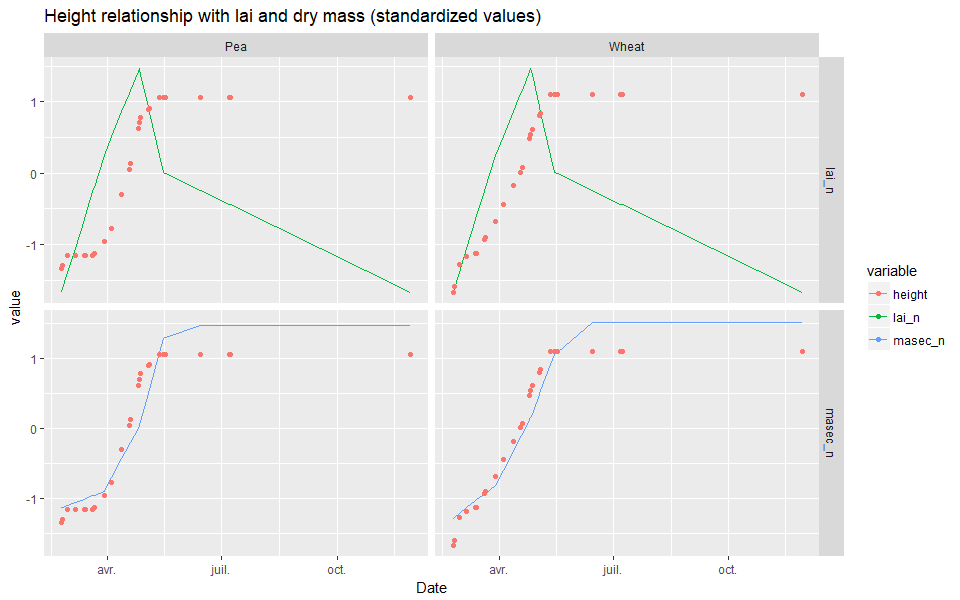
\includegraphics{img/height2.png}
\caption{\label{fig:height2}Observed plant height compared to the lai and dry mass for both wheat and pea in sole crop.}
\end{figure}

The Figure \ref{fig:height2} shows that the plant \texttt{height} is better correlated to the \texttt{masec} than to the \texttt{lai}. We propose to either use the \texttt{masec} or \texttt{somcour} to compute it rather than the \texttt{lai}.

\hypertarget{computing-plant-height}{%
\section{Computing plant height}\label{computing-plant-height}}

\hypertarget{observations}{%
\subsection{Observations}\label{observations}}

The plant \texttt{height} could be computed by either using the plant dry mass (\texttt{masec}) or more simply the development stage, derived from cumulated degree days (\texttt{somcour}).
The second method could be much simpler to parameterize from field, however, both plants experience the same microclimate in STICS for intercrops, so a plant growing dominated by an another plant could have the same cumulative temperature than a plant in sunlit conditions. Hence, this method would not consider the competition effect in interspecies for \texttt{height}, so it cannot be implemented as long as both plants have the same \texttt{somcour}.

To document further this phenomenon, Figure \ref{fig:Peaheight} shows that a Pea grown in intercrop with a wheat has a lower \texttt{height} than a Pea grown in solecrop, and that the dry mass is a good proxy to predict this behaviour.

\begin{figure}
\centering
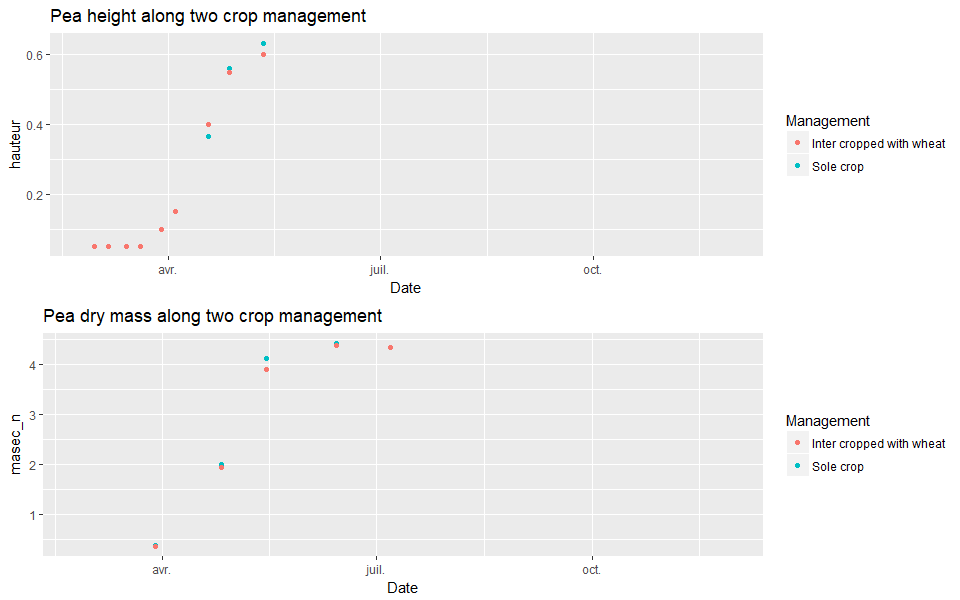
\includegraphics{img/Pea_height.png}
\caption{\label{fig:Peaheight}Observed Pea height and dry mass for a Pea grown in sole crop or in intercrop with wheat.}
\end{figure}

Hence, we will implement a computation of the plant \texttt{height} using the plant dry mass (\texttt{masec}).

\hypertarget{stresses}{%
\subsection{Stresses}\label{stresses}}

Water and nitrogen stresses can both influence the \texttt{height} of a plant. Figure \ref{fig:wheatheightN} shows that the maximum \texttt{height} is reduced for the wheat grown under nitrogen stress (\emph{i.e.} no nitrogen feritilization). However, the \texttt{height} and massec relationship are very close for both management, only the dry mass is higher for fertilized wheat, which gives a higher \texttt{height} in the end.

\begin{figure}
\centering
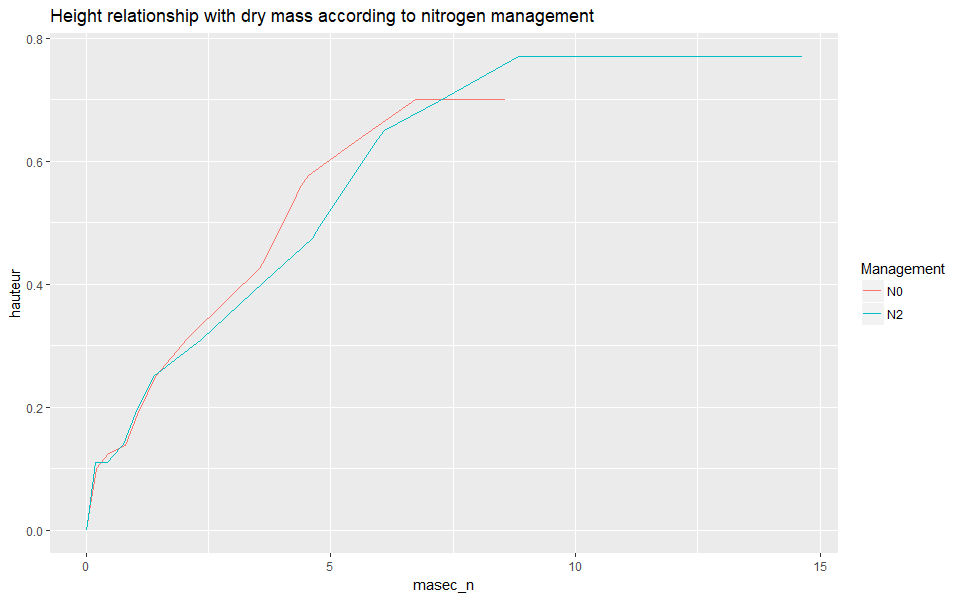
\includegraphics{img/wheat_height_N.png}
\caption{\label{fig:wheatheightN}Observed relationship between height and dry mass for a wheat grown in sole crop.}
\end{figure}

Consequently, height is indeed influenced by nitrogen stress, but it appears from our data that it is only through the \texttt{height\textasciitilde{}masen\_n} relationship. Conequently, the \texttt{height} computation shouldn't be corrected by any nitrogen indices, because this stress is already accounted for in the dry mass computation.

\hypertarget{computation}{%
\subsection{Computation}\label{computation}}

The new computation is implemented in STICS as a new subroutine (\texttt{formplante\_mas}) that is called instead of \texttt{formplante} if the newly defined \texttt{P\_code\_shape} parameter is equal to \texttt{2}. This subroutine is largely based on the previous one, conserving all side effects of \texttt{P\_hautmax}, \texttt{P\_hautmaxtec}, \texttt{P\_largtec} and \texttt{originehaut} but add a computation of the plant height using an allometric relationship with the dry mass as follow :\\
\(hauteur= P_{hautbase} + P_{hautK} \cdot masec^{P_{hautA}}\)

The \texttt{P\_hautbase} parameter is a parameter from \texttt{formplante}, and is used as the intercept of the relationship, \emph{i.e} the base height when the dry mass is equal to 0. \texttt{P\_hautK} is a new parameter that defines the constant of proportionality that reflects the importance of the relationship, and \texttt{P\_hautA} the scaling exponent, or the allometric coefficient. Allometric relationships are simple yet powerfull laws used to describe diverse relationships for wide range of situations. Further documentation can be found on the \href{https://en.wikipedia.org/wiki/Allometry}{wikipedia webpage}.

\hypertarget{results-1}{%
\subsection{Results}\label{results-1}}

Two simulations of a wheat in sole crop and a pea in sole crop were run using STICS to asses the potential of the new computation for height modelling, and the outputs are displayed in Figure \ref{fig:heightWheatSC}.

\begin{figure}
\centering
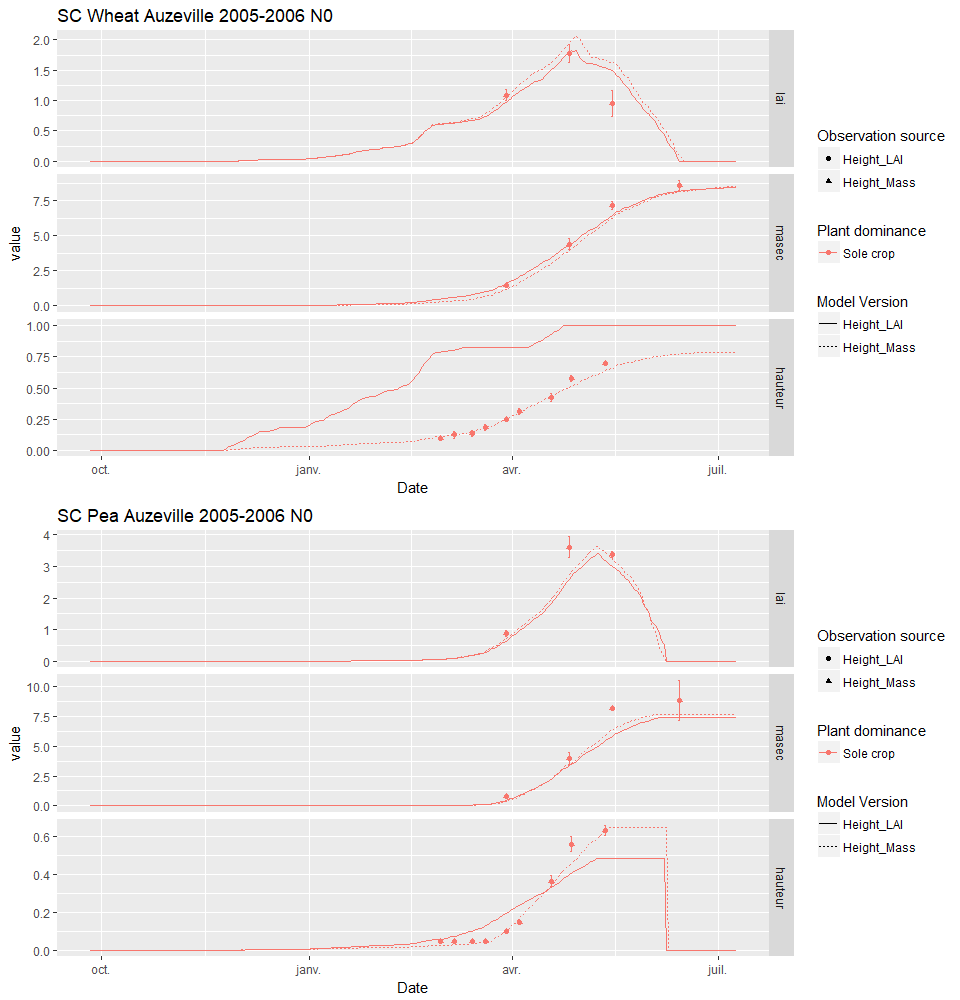
\includegraphics{img/height_Wheat_SC.png}
\caption{\label{fig:heightWheatSC}STICS simulation output for a simulation on two sole crops: wheat and pea}
\end{figure}

The results show that using \texttt{masec} instead of the \texttt{lai} to model plant height gives better results. The model will now be used with this formalism.

\hypertarget{stop-heightmasec-link-at-stage-x}{%
\subsection{Stop height\textasciitilde masec link at stage X}\label{stop-heightmasec-link-at-stage-x}}

The height\textasciitilde masec link can stop existing as soon as a plant reach a certain development stage. For example, wheat stops growing in height from the moment it is flowering.

Hence, a new parameter (\texttt{P\_stage\_const\_height}) was added to have the choice to break this link at any developing stage from this list :

\begin{itemize}
\tightlist
\item
  ``lax'': maximum leaf area index, end or leaf growth.\\
\item
  ``sen'': start of leaf senescene\\
\item
  ``flo'': flowering\\
\item
  ``drp'': start of grain filling\\
\item
  ``mat'': physiological maturity\\
\item
  ``rec'': harvest
\end{itemize}

Figure \ref{fig:constheight} shows the new results, with \texttt{P\_stage\_const\_height=\ flo} for both plants.

\begin{figure}
\centering
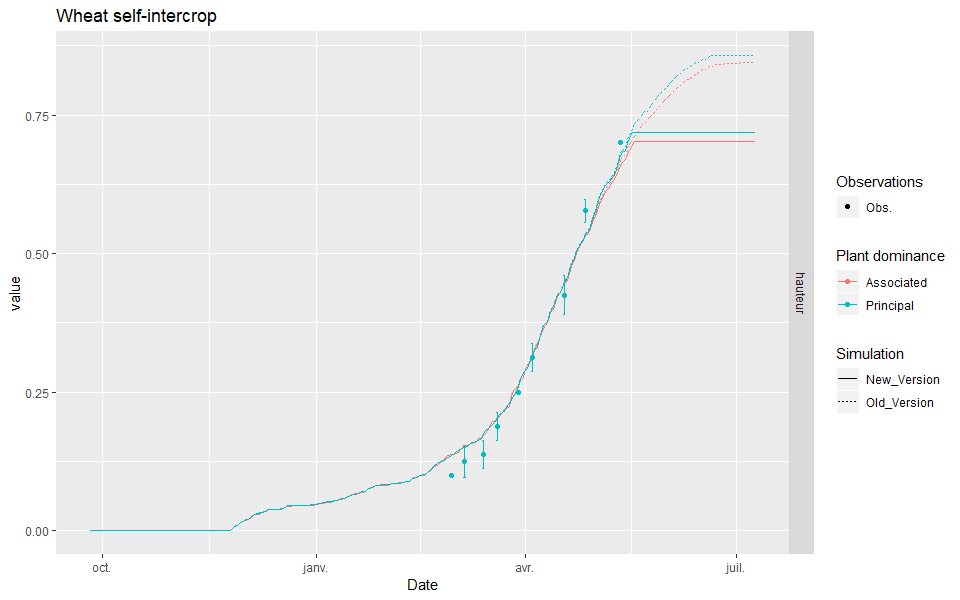
\includegraphics{img/const_height.png}
\caption{\label{fig:constheight}STICS simulation output for a simulation on two sole crops: wheat and pea}
\end{figure}

\hypertarget{stages}{%
\chapter{Developpment stages and LAI dynamic}\label{stages}}

\hypertarget{introduction-8}{%
\section{Introduction}\label{introduction-8}}

Bedoussac (2009) showed the different development stages for the crops, which are reproduced in Figure \ref{fig:stademeas}).

\begin{figure}
\centering
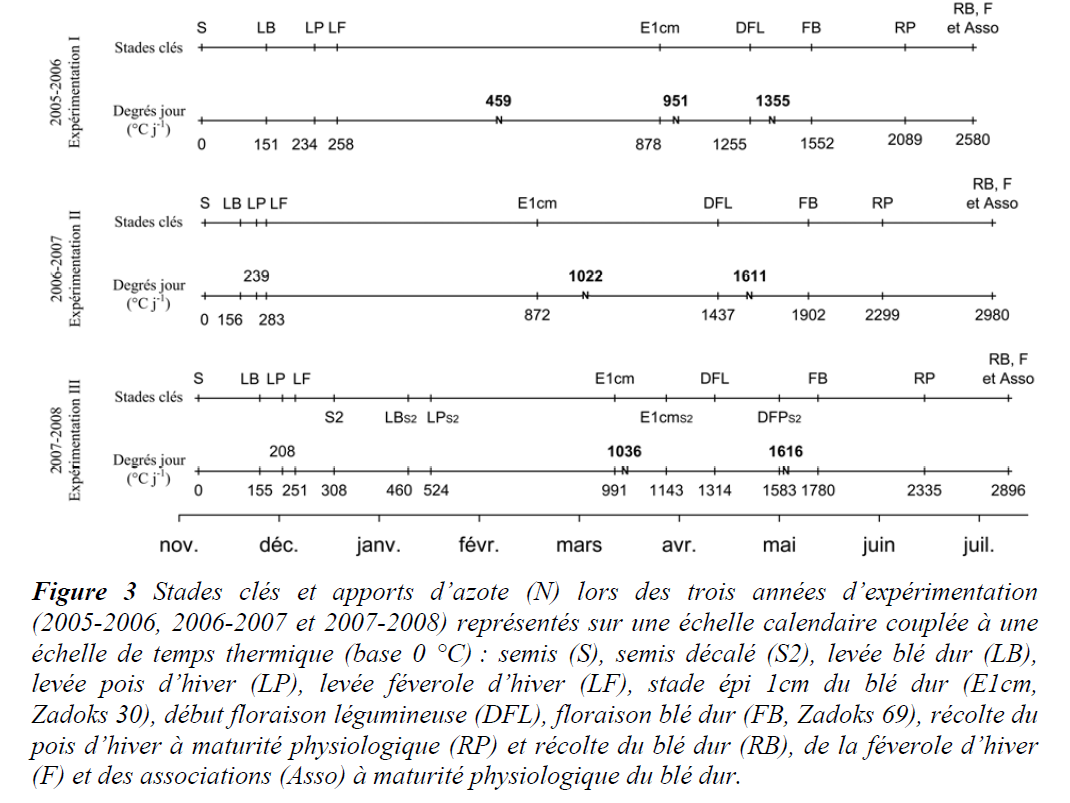
\includegraphics{img/Stades.png}
\caption{\label{fig:stademeas}Development stages as measured in Auzeville}
\end{figure}

The STICS simulations are not in adequation with these results for the moment.

\hypertarget{checking-the-ilev}{%
\section{Checking the ilev}\label{checking-the-ilev}}

The date of emergence is set using the \texttt{ilev} parameter. This parameter had a value of 380 in the STICS input files.

The Fig. 3 of Bedoussac (2009) shows that \texttt{ilev} should occur 151 cumulated Celsius degrees per day after sewing, but a simple computation showed us that this conditions is met on the 329th day already, and not on the 380th as previously parameterized (see computation below).

Figure \ref{fig:ilevIC} and Figure \ref{fig:ilevSC} shows a comparison of some STICS outputs for a wheat self-intercrop and a wheat sole crop respectively, with \texttt{ilev} set either at 380 like before or corrected at 329. The code used to make this output is as follows:

\begin{figure}
\centering
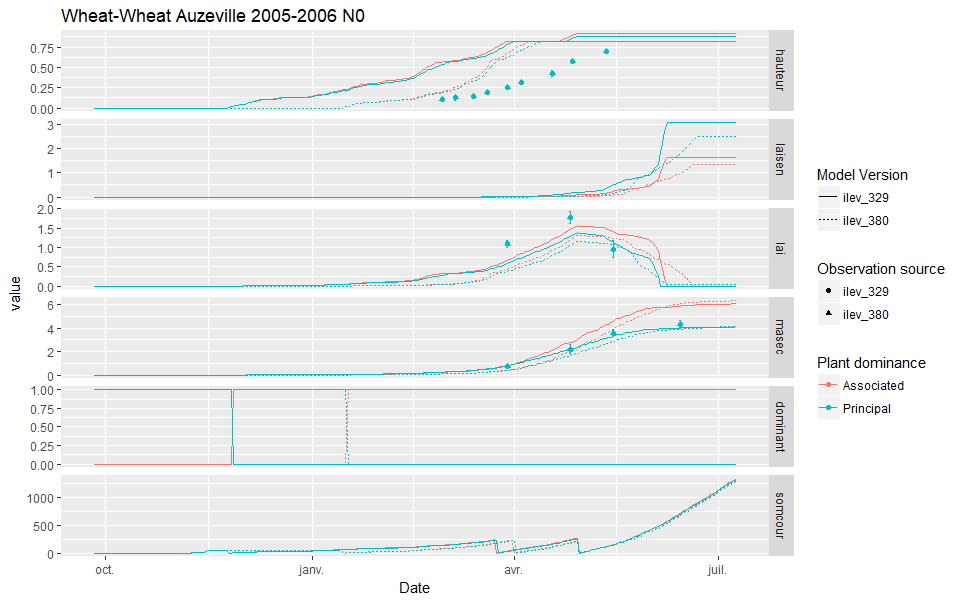
\includegraphics{img/ilev.png}
\caption{\label{fig:ilevIC}STICS outputs comparison with ilev= 380 and corrected to 329 on a wheat-wheat intercropping simulation experiment (Auzeville 2005-2006)}
\end{figure}

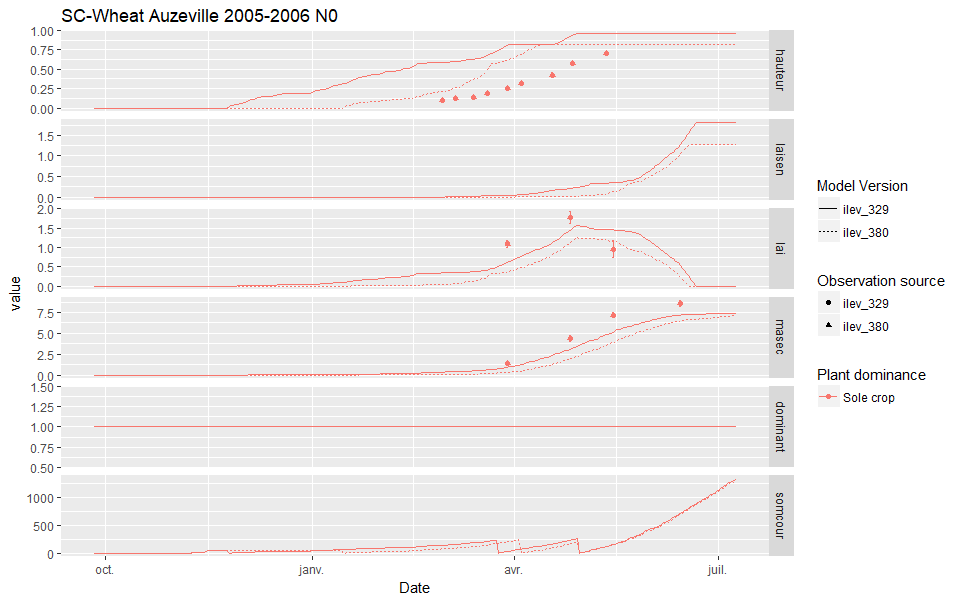
\includegraphics{img/ilevSC.png}
The new parameter values better describe the observations for the development stages, and give simulated \texttt{lai} that are closer to the observations. However, the plant height is now increasing way too soon compared to the observations.

\begin{quote}
These simulations were made using a version of STICS that uses the \texttt{lai} as a proxy for plant height. The model will soon be modified to compute it using other variables.
\end{quote}

\hypertarget{checking-laicomp}{%
\section{Checking laicomp}\label{checking-laicomp}}

The \texttt{laicomp} parameter is used to stop the exponential rate of \texttt{lai} growth, and is set to 0.304 for the moment.
This value could be too low compared to actual conditions, so we increased the value to 0.6 and compared the outputs in Figure \ref{fig:laicomp}).

\begin{figure}
\centering
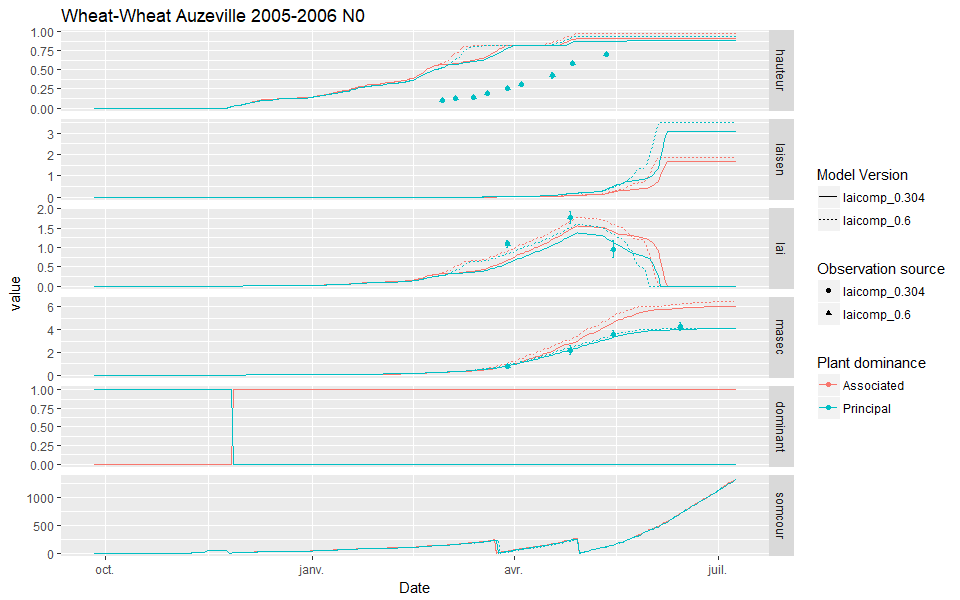
\includegraphics{img/laicomp.png}
\caption{\label{fig:laicomp}STICS outputs comparison with laicomp= 0.304 and corrected to 0.6 on a wheat-wheat intercropping simulation experiment (Auzeville 2005-2006)}
\end{figure}

The new parameterization of \texttt{laicomp} gives simulated \texttt{lai} that are closer to the observations when coupling with the new parameterization of \texttt{ilev}. These two new values (\texttt{ilev}= 329 and \texttt{laicomp}= 0.6) will be kept for future simulations.

\hypertarget{comparing-simulated-and-observed-lai-and-masec-in-self-ic}{%
\section{Comparing simulated and observed lai and masec in self-IC}\label{comparing-simulated-and-observed-lai-and-masec-in-self-ic}}

The simulated \texttt{masec} for each plant of wheat or pea in self-intercrop (\emph{i.e} half the density) was rightfully compared to half the plot-scale observations. However, the \texttt{lai} was wrongly compared to the full observation value, whereas it should be compared to half its value likewise, because the full value has to be compared to the total \texttt{lai}, that is computed by summing both plants \texttt{lai}.\\
The observations were then divided by two to fit the \texttt{lai} simulations outputs that correspond to each plant, so to half values.
The new outputs are shown in Figure \ref{fig:laiobs}). The modification tells us that the plant \texttt{lai} is overestimated in self-intercrop.

\begin{figure}
\centering
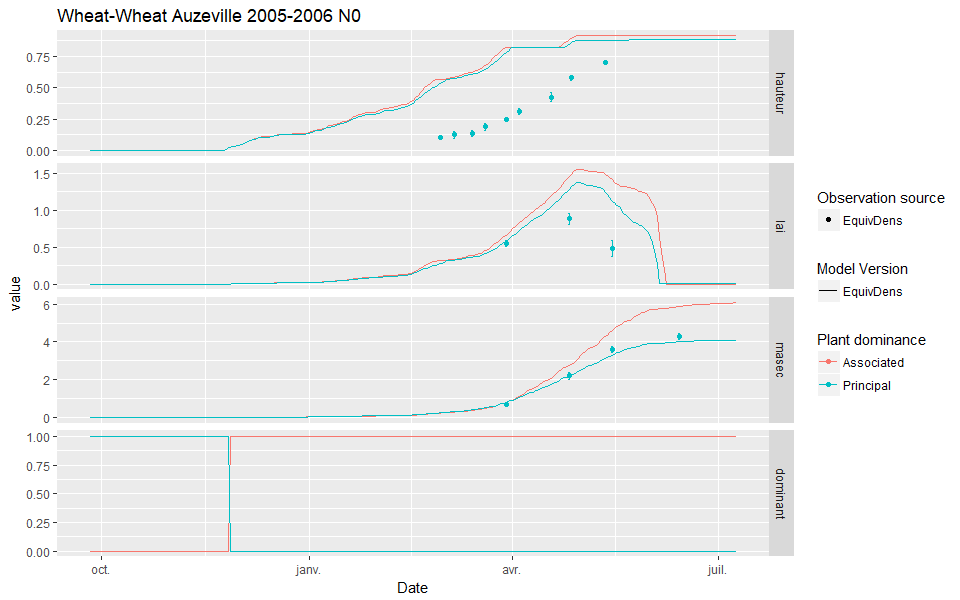
\includegraphics{img/laiobs.png}
\caption{\label{fig:laicomp}STICS outputs comparison with half lai values on a wheat-wheat intercropping simulation experiment (Auzeville 2005-2006)}
\end{figure}

\hypertarget{checking-durviei}{%
\section{Checking durvieI}\label{checking-durviei}}

The lifespan of the early leaves is expressed as a proportion of the lifespan of the late leaves, and is called \texttt{durvieI}. This parameter help control the steepness of the decreasing part of the \texttt{lai} through leaf mortality (\emph{i.e.} senescence).\\
It appears that the leaf senescence is not well simulated in the wheat sole crop, because the \texttt{lai} do not drop as fast as in the observations. We propose to decrease the value of \texttt{durvieI} from 0.8 to 0.6. A comparison of the effect of changing this value is shown in Figure \ref{fig:durvieISC}) for sole crop and for \ref{fig:durvieIIC}) self-intercrop.

\begin{figure}
\centering
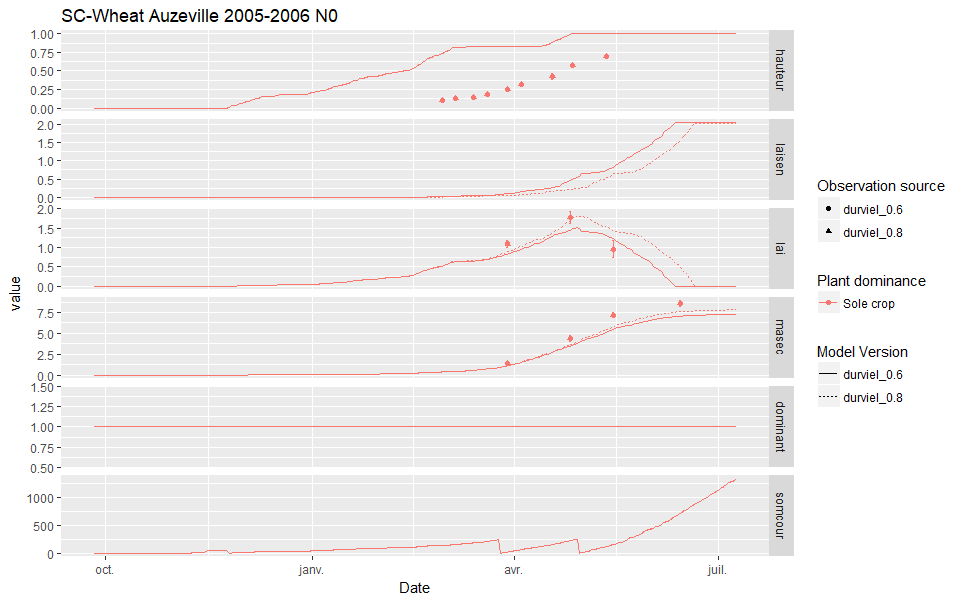
\includegraphics{img/durvieISC.png}
\caption{\label{fig:durvieISC}STICS outputs comparison with durvieI= 0.8 compared to 0.6 on a wheat sole crop simulation experiment (Auzeville 2005-2006)}
\end{figure}

\begin{figure}
\centering
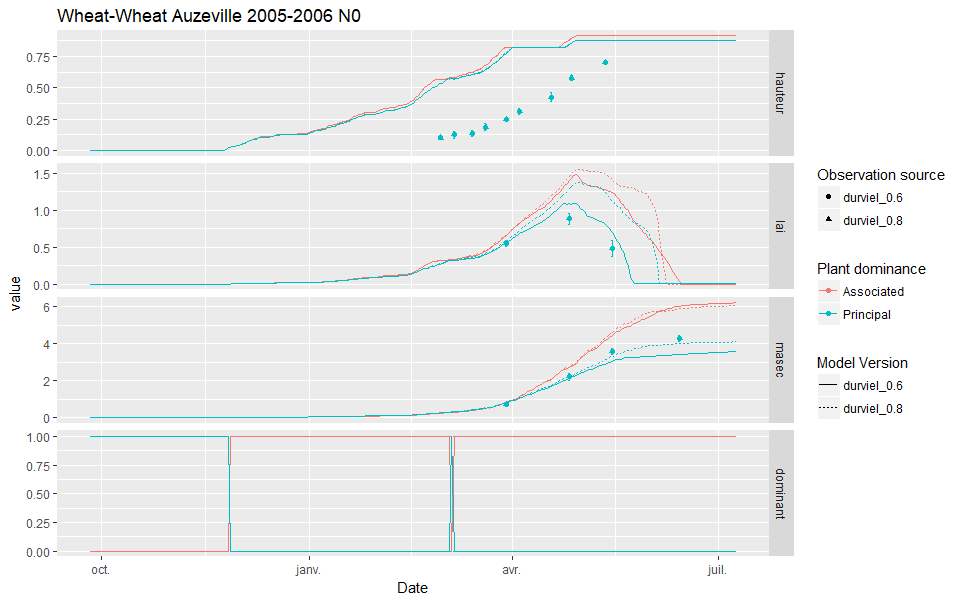
\includegraphics{img/durvieIIC.png}
\caption{\label{fig:durvieIIC}STICS outputs comparison with durvieI= 0.8 compared to 0.6 on a wheat-wheat intercropping simulation experiment (Auzeville 2005-2006)}
\end{figure}

\hypertarget{LAItoohigh}{%
\chapter{The LAI in intercropping is too high}\label{LAItoohigh}}

\hypertarget{introduction-9}{%
\section{Introduction}\label{introduction-9}}

The \texttt{LAI} is too high compared to observations for intercropping. This is especially visible while making a self-intercrop (\emph{i.e} wheat-wheat or pea-pea) simulation compared to a sole crop, as shown in Figure \ref{fig:LAItoohigh}.

\begin{figure}
\centering
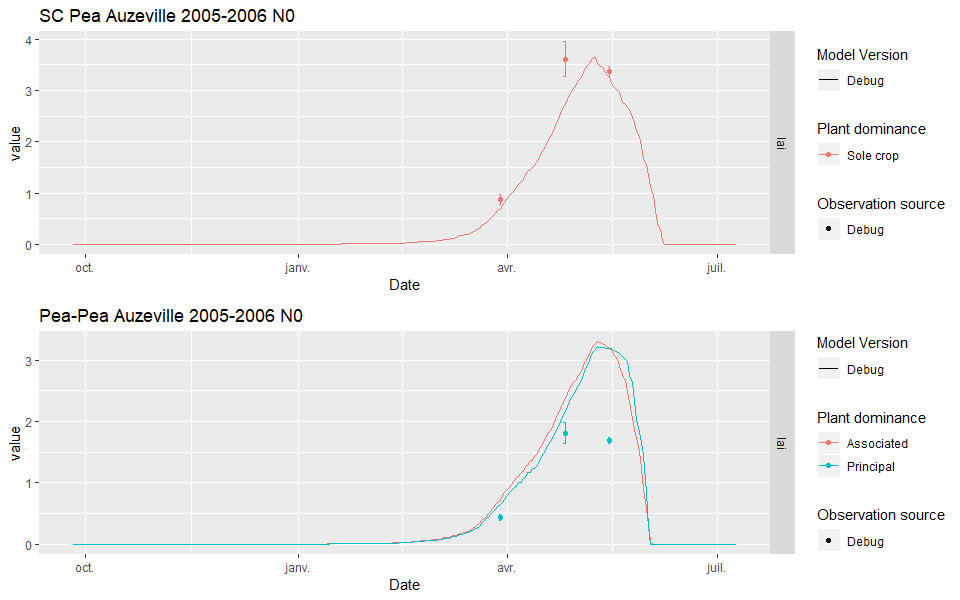
\includegraphics{img/LAI_high_PP.png}
\caption{\label{fig:LAItoohigh}Leaf Area Index in a Pea sole crop and in a self-intercrop of Pea-Pea}
\end{figure}

This issue probably rise from the computation of \texttt{deltai}, and the main hypothesis are:

\begin{itemize}
\tightlist
\item
  \texttt{P\_dlaimax} is not well parameterized.\\
\item
  \texttt{ulai} is not well simulated in intercrop.\\
\item
  \texttt{efdensite} and \texttt{densite} are not well simulated. The value of the density used in the \texttt{deltai} equation in the self-intercrop should be half the value of the sole crop.
\end{itemize}

The first hypothesis is rejected because the \texttt{lai} simulation is close to the measurements in the sole crop, so it should perform equally in intercrop because \texttt{P\_dlaimax} should have the same value in sole crop and in intercrop.

\hypertarget{investigating-the-ulai-hypothesis}{%
\section{\texorpdfstring{Investigating the \texttt{ulai} hypothesis}{Investigating the ulai hypothesis}}\label{investigating-the-ulai-hypothesis}}

Figure \ref{fig:ulai} shows that both the sole crop (SC) and self-intercrop (IC) simulations yield approximately the same \texttt{ulai} throughout the crop cycle. This discard the second hypothesis.

\begin{figure}
\centering
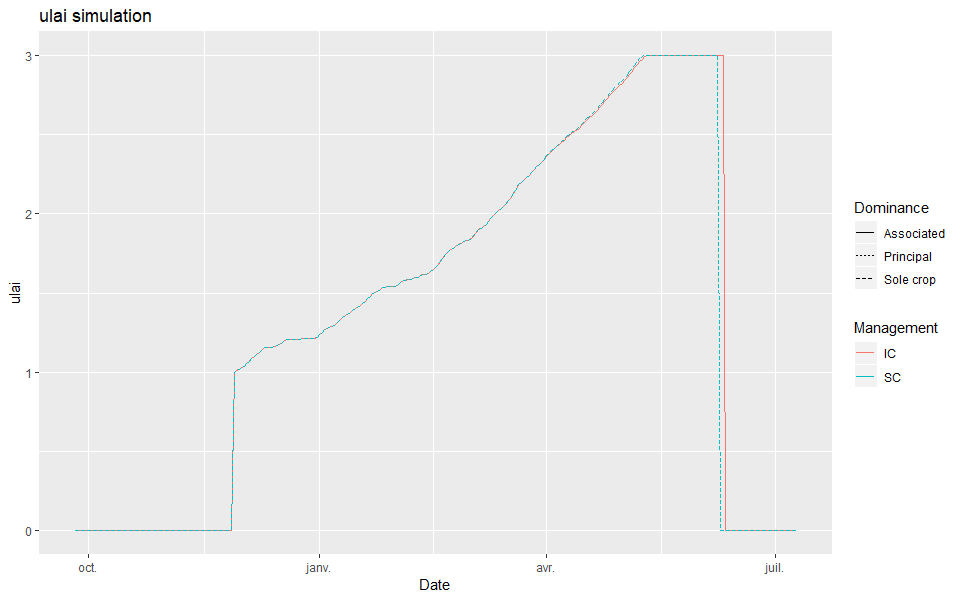
\includegraphics{img/ulai_laitoohigh.png}
\caption{\label{fig:ulai}Simulated ulai in a self-intercrop of Pea-Pea compared to a sole crop of Pea}
\end{figure}

\hypertarget{investigating-the-density-hypothesis}{%
\section{Investigating the density hypothesis}\label{investigating-the-density-hypothesis}}

Figure \ref{fig:densiteef} shows that the density in the Pea self-intercroping is higher than expected. The issue probably come from this.

\begin{figure}
\centering
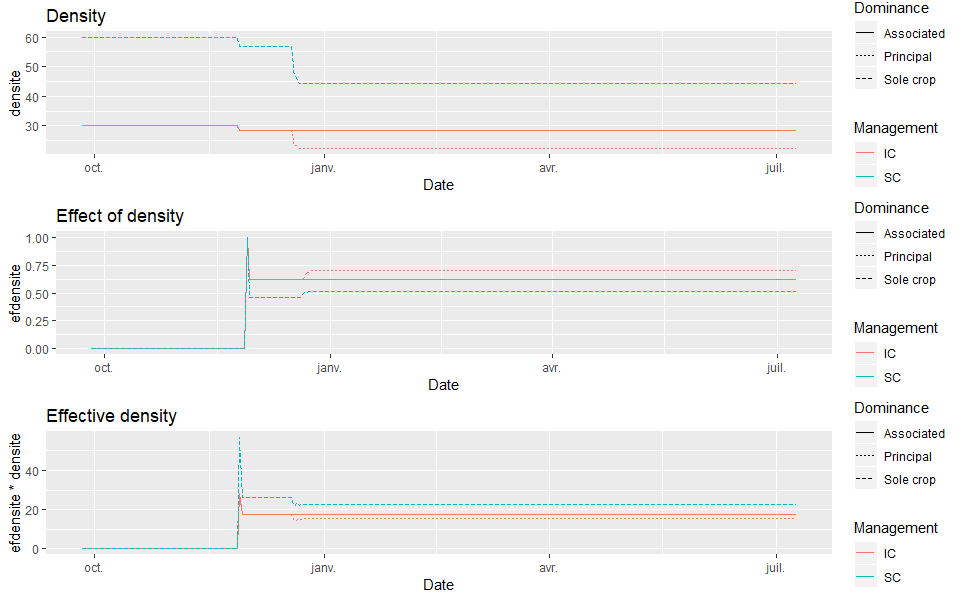
\includegraphics{img/density_effect.png}
\caption{\label{fig:densiteef}Simulated densite, efdensite and the resulting density from their multiplication in a self-intercrop of Pea-Pea compared to a sole crop of Pea}
\end{figure}

Furthermore, we can see that the plant density is reduced twice for both Pea in SC and for the dominant plant in IC. The first is because some plants are lost in the first growing stage (\texttt{densite\_lev}), and the second because of frost damage. However, the frost does not affect the associated plant density in IC. This does not reflect reality and should be changed.
The error came from a piece of code in the \texttt{senescen} subroutine where the computation differed between dominant and dominated plants.

The code was changed into only one condition for both plants:

\begin{quote}
SHA: f525211036a7b4b683252093187298324f4cd80b
\end{quote}

The code modification lead to better results, with an effect of frost that is equal between dominant and dominated plants as seen in Figure \ref{fig:densitefrost}.

\begin{figure}
\centering
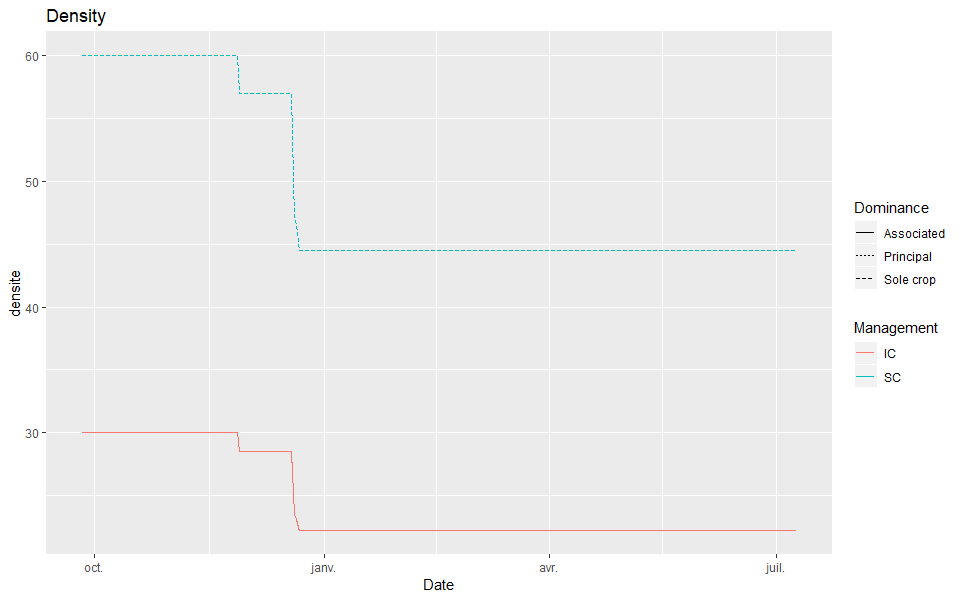
\includegraphics{img/densitefrost.png}
\caption{\label{fig:densitefrost}Simulated density in a self-intercrop of Pea-Pea compared to a sole crop of Pea. NB: Both plants density have the same value in the self-intercrop (half the value of sole crop)}
\end{figure}

However, an evaluation of the model on Auzeville data showed that the problem of a high \texttt{lai} persisted, so the issue did not come from this bug alone.
More investigation showed that \texttt{efdensite} was lower in self-intercrops compared to sole crop simulations, because the equivalent density of both dominant and dominated plants were set equal to the plant density or higher for the dominated plant if the difference in height is large (see Chapter \ref{plantdensity}). However, the plant equivalent density should refer to the plant density as if it were in sole crop to have the same density effect while using sole crop parameters for \texttt{efdensite}, and not to be equal to the half-density, as it is for the moment.\\
The equivalent density computation was then modified to match a density equivalent to a sole crop density, that is to say, twice the value of the sowing density in intercrop, \emph{i.e.} the same density as if the other plant was from the same species.

As expected, the code modification led to the simulation of the same \texttt{efdensite} in SC and in IC for both plants, as seen in Figure \ref{fig:efdensite}.

\begin{figure}
\centering
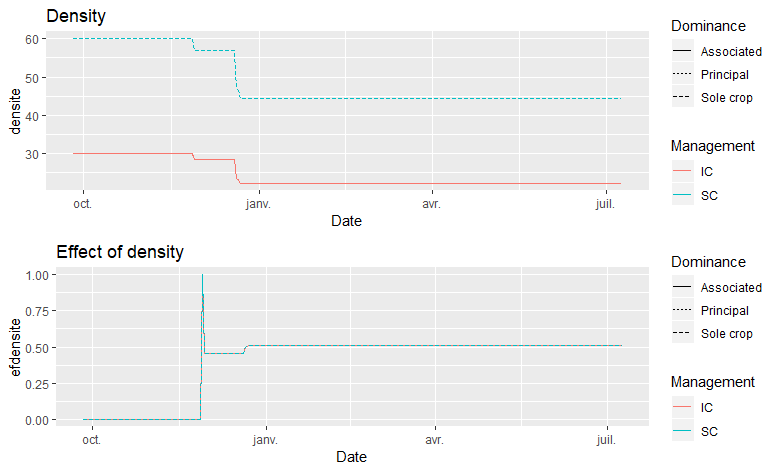
\includegraphics{img/efdensite.png}
\caption{\label{fig:efdensite}Simulated density and density effect in a self-intercrop of Pea-Pea compared to a sole crop of Pea. NB: Both plants density have the same value in the self-intercrop (half the value of sole crop), all plants/managements have the same value of efdensite.}
\end{figure}

\hypertarget{misc}{%
\chapter{Miscellaneous}\label{misc}}

\hypertarget{introduction-10}{%
\section{Introduction}\label{introduction-10}}

This chapter keep trace of several little issues resolved rapidly and with no high significance.

\hypertarget{extra-code-from-transrad}{%
\section{Extra code from transrad}\label{extra-code-from-transrad}}

Some pointless code was present in the \texttt{kgeom} subroutine in the \texttt{transrad.f90} file. The code assignated values to the \texttt{kg} variable twice in a row, and then \texttt{kg} was always recomputed anyway:

We propose to remove the \texttt{if...endif} code bloc. The effect of the removal of this part of code was tested against the Auzeville dataset, and as expected no change was observed in the outputs.

\hypertarget{sowing-density-in-auzeville}{%
\section{Sowing density in Auzeville}\label{sowing-density-in-auzeville}}

The sowing density in Auzeville was set to 168 for the wheat at half-density in intercropping. We change that to the real value of 140 instead.

\hypertarget{energy-balance}{%
\section{Energy balance}\label{energy-balance}}

A new variable was added in STICS to keep track of the plant layers net radiation to make an energy balance. This variable is called \texttt{rnet\_plant}, and is computed in the \texttt{shutwall} subroutine. It is computed using the radiation intercepted by each plant layer. The net radiation is computed as:

\(rnet= rnet_{plant_1}+rnet_{plant_2}+rnet_{soil}\)

Now it can be checked ad hoc using the new outputs, such as shown in Figure \ref{fig:netradiation} that shows as expected that the net radiation output from STICS (\emph{i.e.} \texttt{rnet}) is equal to the sum of the net radiation of the dominant (\texttt{p(1)\%rnet\_plant}) and dominated (\texttt{p(2)\%rnet\_plant}) plant as well as the net radiation from the soil (\texttt{rnetS}).

\begin{figure}
\centering
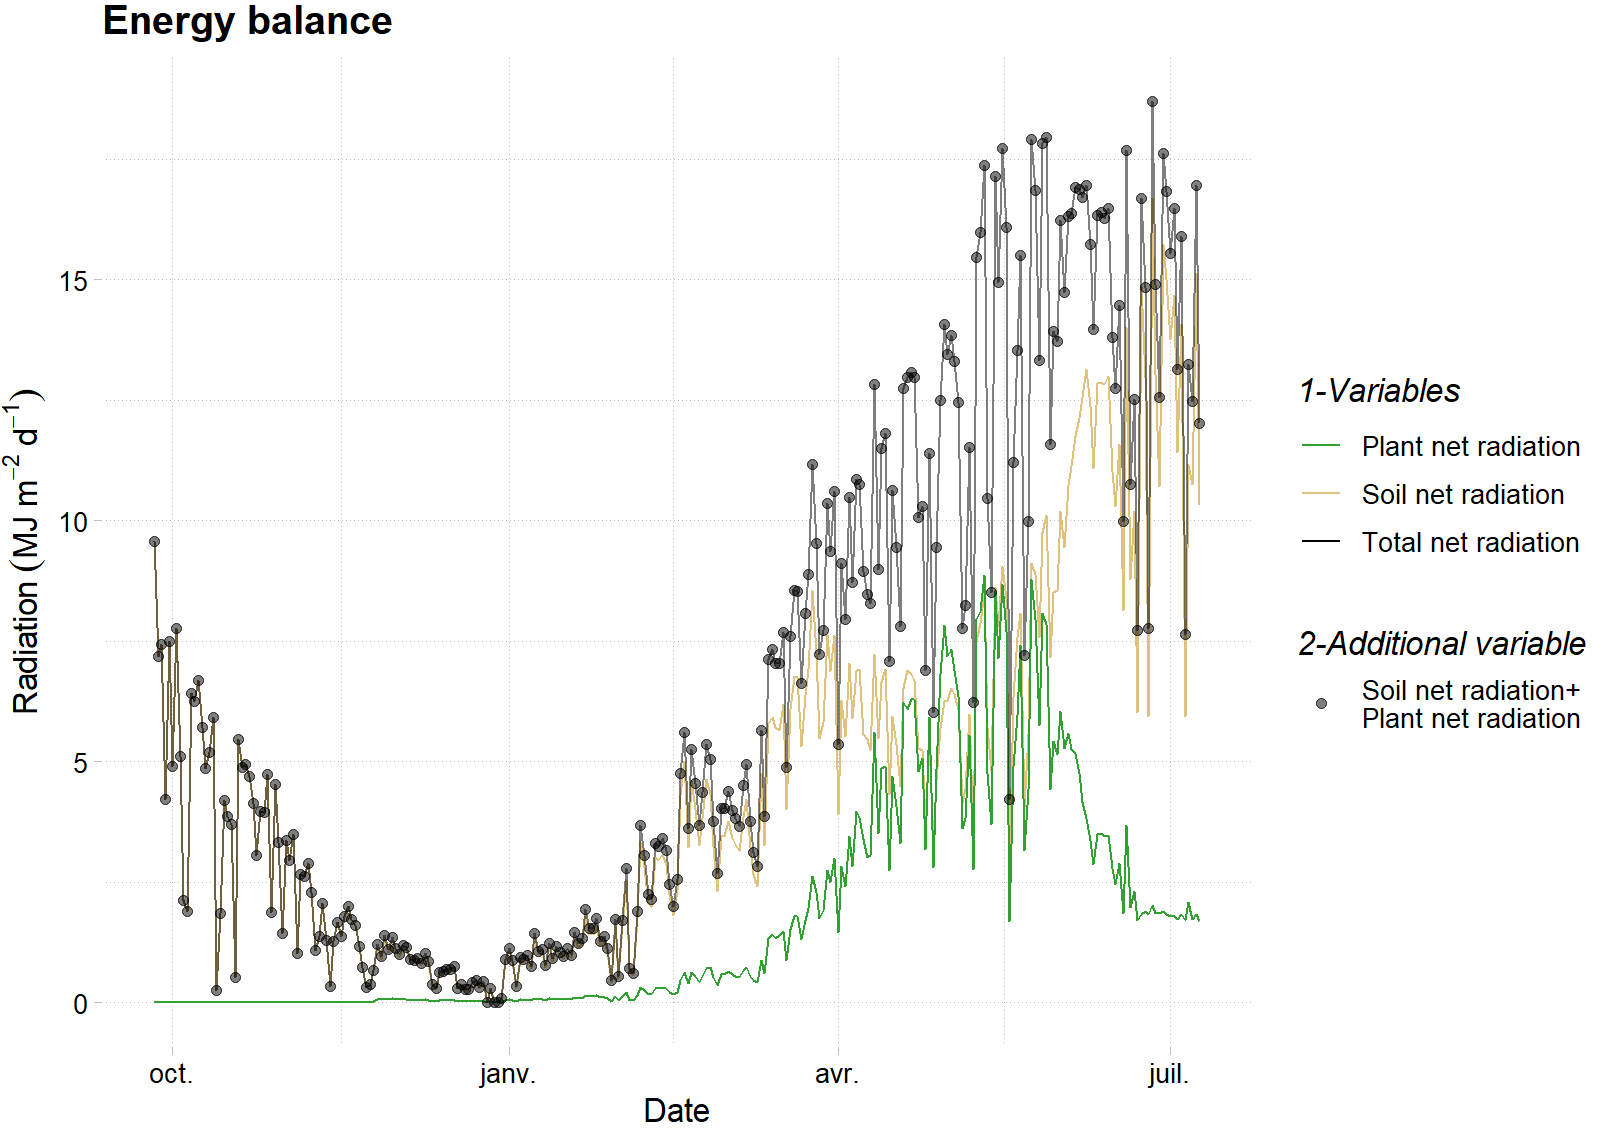
\includegraphics{img/energy_balance.png}
\caption{\label{fig:netradiation}Net radiation computed in the model and out of the model}
\end{figure}

\hypertarget{positive-raint-with-zero-laieai}{%
\section{Positive raint with zero LAI+EAI}\label{positive-raint-with-zero-laieai}}

\texttt{raint} was not equal to 0 (and so \texttt{fapar}) when the \texttt{lai}+\texttt{eai} was equal to 0, instead it remained at the last computed value when \texttt{lai}+\texttt{eai} was \textgreater0. A little modification of the model was made to fix the bug as seen in Figure \ref{fig:bugraint}. Note that a little modification on the computation of leaf senescence fix also a bug for the \texttt{lai} at the end (see e027b8efd93fe77aa7ac7242ce3496589003eb41).

\begin{figure}
\centering
\includegraphics{img/raintbug.png}
\caption{\label{fig:bugraint}Bug fix for raint when lai+eai=0}
\end{figure}

\hypertarget{qfix-decrease}{%
\section{Qfix decrease}\label{qfix-decrease}}

S. Munz discovered that Qfix decreased abruplty in some years in intercropping. This effect should not be possible because Qfix is the cumulative fixed nitrogen.
The issue was corrected in commit \texttt{4f9d92595c870d9b08f3f0b986cbb321630ad031}. The results are shown in figure \ref{fig:Width}.

\begin{figure}
\centering
\includegraphics{img/Qfix_issue.png}
\caption{\label{fig:Qfix}\textbf{Issue with Qfix decreasing abruptly for Pea. Principal plant: Pea, Dominated: Wheat. Simulation for 2007, low nitrogen (N0)}}
\end{figure}

\hypertarget{efdensite_rac}{%
\section{efdensite\_rac}\label{efdensite_rac}}

The effect of the density on the roots (\texttt{efdensite\_rac}) was computed using the current plant density, bt for intercrops it should use \texttt{densiteequiv} because the parameters are fitted using a sole crop equivalent density. This computation was fixed in commit \texttt{ba45c6c73d1bb9a081393e84f648a9c90bf47428}.

\hypertarget{summary1}{%
\chapter{First summary}\label{summary1}}

\hypertarget{introduction-11}{%
\section{Introduction}\label{introduction-11}}

A lot of code and parameterization has changed since the beginning of this book. Here is a little summary of all changes, starting with the outputs we have at this stage, followed with a step-by-step parameterization help for the new formalism.

\hypertarget{model-outputs}{%
\section{Model outputs}\label{model-outputs}}

The model was tested on a series of experimentations on Wheat and Pea from Auzeville. It consists on a set of observations made on either sole crops or intercrops, and the model was run on each case to evaluate its simulation outputs. The model was also tested to simulate a sole crop as an intercrop with both plants from the same species and variety.\\
The results of this evaluation are available on \href{Auzeville_summary.html}{this separate page}.
You can consider this page as a snapshot of the evaluation of the model version used as : 31 mars, 2020. This version of the model can be retrieved from my GIT repository using this SHA: \texttt{c9638aafb924949b630d273608d2b3c45369cd0c}.

\hypertarget{model-parameterization}{%
\section{Model parameterization}\label{model-parameterization}}

\hypertarget{height-1}{%
\subsection{Height}\label{height-1}}

The height can be computed using two different paradigms:

\begin{itemize}
\tightlist
\item
  The previous one, that uses the plant \texttt{lai} and foliar density (which depends also on the \texttt{lai}) to compute the plant width, and then uses a ratio to retrieve the plant height.\\
\item
  The new one that simply links the plant dry mass (\texttt{masec(n)}) to its height using an allometric relationship.
\end{itemize}

The computation is chosen using the \texttt{P\_code\_shape}. If \texttt{P\_code\_shape} is equal to \texttt{2}, the model will use the second one (using \texttt{masec}), and for any other value, it will use the first one.

The allometric equation is simply defined as:\\
\(hauteur= P_{hautbase} + P_{hautK} \cdot masec^{P_{hautA}}\)\\
So it has two new parameters: \texttt{P\_hautK} and \texttt{P\_hautA}.
This equation is well known across a wide range of fields, can describe a large panel of relationships, is robust, and is quite simple to parameterize. In the case of STICS, the user should use sole crop data only for parameterization, because the hauteur\textasciitilde masec relationship is hard-coded for this situation. In the case of intercrop, the model will adapt the computation accordingly.

For our case experiment in Auzeville, these parameters were fitted thanks to the nls function in R using observations for each species independently.

At first, we were afraid that the relationship would differ according to the nitogen management, but only the dry mass was impacted by the nitrogen treatments, not the height\textasciitilde masec relationship. However, the relationship changed a little between sole crops and intercrops, but was still robust enough to use it as is as shown in the results from \href{Auzeville_summary.html}{this separate page}, also shown in the first paragraph.

\hypertarget{equivalent-density}{%
\subsection{Equivalent density}\label{equivalent-density}}

The equivalent density is the density the plant would have if the other plant was of the same species, \emph{i.e.} if the field was a sole crop. This equivalent density is used to compute the plant \texttt{LAI}. It is computed in three different ways in STICS, that are all described in Chapter \ref{plantdensity}. The third computation is re-explained here for ease:

The third formalism is chosen by setting \texttt{P\_code\_calc\_equi\_density=3}. It is an improved computation to define the equivalent density as a function of the height difference between the plants, and using different parameters for intraspecific and interspecific competition, with simpler meanings. This formalism gives an equivalent density equal to the double of the true density to match a density equivalent to a sole crop, and increases this equivalent density until a given threshold (\texttt{hauteur\_threshold}), after which a progressive increase in the equivalent density happen until the maximum allowed. In this computation, the slope is computed by the model, and the equivalent density is computed as follows:\\
\(density_{Equivalent} =\begin{cases}\Delta_{height} < hauteur_{threshold} & density_{p2} \\ \Delta_{height} > hauteur_{threshold} & b + \Delta_{height}\cdot slope \\ \Delta_{height} > hauteur_{threshold_2} & Max_{equDens} \end{cases}\)\\
with \(slope= \frac{Max_{equDens}}{hauteur_{threshold_2}-hauteur_{threshold}}\).

Hence, this formalism include three parameters (named here as used in the model):

\begin{itemize}
\tightlist
\item
  \texttt{P\_hauteur\_threshold}: the difference in height below which no competition is occuring
\item
  \texttt{P\_hauteur\_threshold\_2}: the difference in height below which a progressive competition is occuring
\item
  \texttt{P\_eqdens\_max}: the maximum density allowed in intercrop, \emph{i.e.} generally the sole crop density.
\end{itemize}

These three parameters are quite simple to parameterize also. The first one should be set to represent the moment the height difference between two plants start increasing competition. We set this parameter to 0.2 meters, because we considered no competition increase before a difference of 20 centimeters between both plants. The second threshold was set to 0.8 meters, because we considered the competition would increase linearly until this difference in height, reaching its maximum at this point. The \texttt{Max\_equDens} was set to 240 for wheat and 60 for Pea. These densities correspond to a full density in a sole crop.

\begin{quote}
Note: the increased equivalent density with height or whatever formalism used is only there to represent competitions comming from other processes than light interception, as it is already accounted for by the light interception subroutines. The model must be well parameterized for the light interception first, using no increase in equivalent density first (\emph{e.g.} by setting a high \texttt{P\_hauteur\_threshold}), and then the equivalent density formalism can be used to better match the plants competition if needed.
\end{quote}

\hypertarget{intercfix}{%
\chapter{Interception fix}\label{intercfix}}

\hypertarget{introduction-12}{%
\section{Introduction}\label{introduction-12}}

When simulating a self-intercrop, \emph{i.e.} a monocrop simulated as if it was an intercrop, both plants outputs were quite different.

This was arising from the computation of the light competition between the two plants: one was considered dominant over the other one, so the received by the dominated plant was only the light transmitted by the other.

This computation needed to change, so we included two cases to compute the light incident to the plants:

\begin{enumerate}
\def\labelenumi{\arabic{enumi}.}
\item
  The dominant plant is considered above the dominated plant (dominancy case): \texttt{p(i-1)\%rsoleil} represents the fraction of the radiation incoming right above the plant i, i.e.~the light transmitted to the associated plant, for the sunlit part (rombre is used for the shaded one). So \texttt{trg\_bak\ *\ p(i-1)\%rsoleil} is the actual amount of radiation transmitted to the sunlit part of the associated plant, and \texttt{trg\_bak\ *\ p(i-1)\%rombre} is the actual amount of radiation transmitted to the shaded part of the associated plant.
\item
  There is no clear dominancy because both plants have approx. the same height (Delta height\textless hauteur\_threshold): the trg is not transmitted from one plant to the other, but shared between both plants. In that case, the competition for light arises only through the LAI of each plant.
\end{enumerate}

The new version of the model integrating this code can be retrieved from the repository using this SHA: \texttt{591cd8db5aeaf8db2cdb5b62008c54d04d833df8}.

\hypertarget{model-parameterization-1}{%
\section{Model parameterization}\label{model-parameterization-1}}

The model does not need any further parameterization because this new formalism uses one parameter that is already available: \texttt{hauteur\_threshold}.

\hypertarget{lightcompetition}{%
\chapter{Light competition effect}\label{lightcompetition}}

The competition between the plant species in intercropping was so much mixed between several computations that it became difficult to parameterize the models, or even to grasp the functionning of the model. We propose a brand new approach to clarify and simplify the computations, while including a new process in the model: the shoot elongation.

As explained in chapter \ref{Light}, STICS considers two kinds of competitions for light: the intra-species competition, and the inter-species competition. The model computes a competition for light between both species using the light interception module, and a second competition using the plant density. Until now the density effect represented both intra and inter-species competition because it was computed using an ``equivalent'' density that increased with the difference in height between the plants (see \ref{plantdensity}). This equivalent plant density was difficult to explain, and difficult to parameterize because it was used to compute \texttt{efdensite} (the density effect) with the same equation than for a sole crop, where this density effect is only an intra-specific competition.

The model should simulate approximately the same results simulating a sole crop or the same crop twice in intercrop (we call it a self-intercrop). It was difficult make the model do it because the same equations were used for different purposes, so the parameterization of the model did not stand well.

We propose to remove the complicated computation of the equivalent density because the competition for light between the two plants is already considered in the light interception module. We argue that the density computation should only be used for the same purpose as for the sole crop (intra-specific competition) to correctly use the \texttt{adens} and \texttt{bdens} parameters that are parameterized for a sole crop. The equivalent density would be used only as a way to match the density in intercrop to the equivalent density it would have in the sole crop, i.e.~densite*2 (densite: sowing density). The density effect (\texttt{efdensite}) would then only represent the intra-row competition, and the inter-row competition would be computed using the light interception module.

It would greatly simplify the processes involved in intercropping, reducing the number of parameters with a complex meaning : \texttt{hauteur\_threshold2}, \texttt{eqdens\_max1}, \texttt{eqdens\_max2} and \texttt{code\_calc\_equi\_density}.
\textgreater{} \texttt{P\_hauteur\_threshold} is still needed to know when we consider the plants are starting to be in competition for light.

We also want to add another important process to the model: the elongation of the shoot with increasing shade. We propose to add a computation for the shoot elongation effect (called \texttt{ef\_elongation}) that would be applied to increase the plant heigth with increasing shading. This computation adds only one parameter that represent the effect on plant heigth with the maximum shading. This parameter is called \texttt{P\_elongation}.

The computation is as follow:

with \texttt{surf\_AO} the relative surface of the plant that is shaded (0.0: full sun, 1.0: fully shaded), \texttt{P\_elongation} the elongation effect when the plant is fully shaded (1.0 - n), and \texttt{ef\_elongation} the resulting elongation effect that is applied to compute the plant heigth. \texttt{ef\_elongation} linearly increases with increasing shading.

The following plot shows the elongation effect with \texttt{P\_elongation=\ 1.5} for an increasingly shaded plant.

\includegraphics{Postdoc_steps_files/figure-latex/unnamed-chunk-37-1.pdf}

The elongation effect is then applied to the computation of the heigth as follows:

By modifying our previous approach, we hope to simplify the computation of the competition for light between plants, and to integrate a potentially essential process that is shoot elongation. We can summarize the new approach as follows:

\begin{itemize}
\item
  The intra-species competition is computed as it is in sole-crops using \texttt{efdensite}
\item
  The inter-species competition is computed using the light interception module
\item
  The plant elongation is also computed using the light interception module with the relative shaded surface of the plant as a proxy for light quality.
\end{itemize}

  \bibliography{book.bib,packages.bib}

\end{document}
